\documentclass[12pt,a4paper]{article}
\usepackage[utf8x]{inputenc}
\usepackage{setspace}
\usepackage[german]{babel}
\usepackage{graphicx} 
\usepackage[T1]{fontenc}
\usepackage{amsmath}
\usepackage{amsfonts}
\usepackage{amssymb}
\usepackage{url}
\usepackage[bf]{caption}
\usepackage[a4paper]{geometry}
\usepackage{float}
\usepackage{acronym}
\usepackage{pdfpages}
\usepackage{enumitem}
\usepackage{wrapfig}

\usepackage{jurabib}

\jurabibsetup{
	commabeforerest,
	ibidem=strict,
	%here you can change full citation, none, first
	citefull=first,
	see,
	titleformat={colonsep,all},
}

\renewcommand*{\jbauthorfont}{\textsc}
\renewcommand*{\biblnfont}{\scshape\textbf}
\renewcommand*{\bibfnfont}{\normalfont\textbf}
\AddTo\bibsgerman{%
	\renewcommand*{\ibidemname}{ebd.}
	\renewcommand*{\ibidemmidname}{ebd.}
}

\usepackage[bottom,hang]{footmisc}
\setlength{\footnotemargin}{0pt}


% Für source codes etc.
\usepackage{listings}

\usepackage{color}
\definecolor{gray}{rgb}{0.4,0.4,0.4}
\definecolor{darkblue}{rgb}{0.0,0.0,0.6}
\definecolor{cyan}{rgb}{0.0,0.6,0.6}

\lstset{
  numbers=left,   
  basicstyle=\ttfamily,
  columns=fullflexible,
  showstringspaces=false,
  commentstyle=\color{gray}\upshape
}

\lstdefinelanguage{XML}
{
  basicstyle=\footnotesize\ttfamily,
  morestring=[b]",
  morestring=[s]{>}{<},
  morecomment=[s]{<?}{?>},
  stringstyle=\color{black},
  identifierstyle=\color{darkblue},
  keywordstyle=\color{cyan},
  morekeywords={xmlns,version, type, about, resource, lang}
  % list your attributes here
}

\geometry{a4paper,left=25mm,right=25mm, top=25mm, bottom=25mm}
\onehalfspacing
\renewcommand{\familydefault}{ptm}

\usepackage[bottom,hang]{footmisc}
\usepackage{fnpct}


\setlength{\footnotemargin}{0pt}

\setlength{\parindent}{0pt}


\author{Christopher Pollin}
\title{\textbf{Formale, digitale Methoden und Modelle in den Geschichtswissenschaften. Am Beispiel digital edierter Rechnungsbücher}}
\date{\today{}, Graz}
\begin{document}
\pagenumbering{gobble}
\AdaptNoteOpt\footcite\multfootcite

%\maketitle
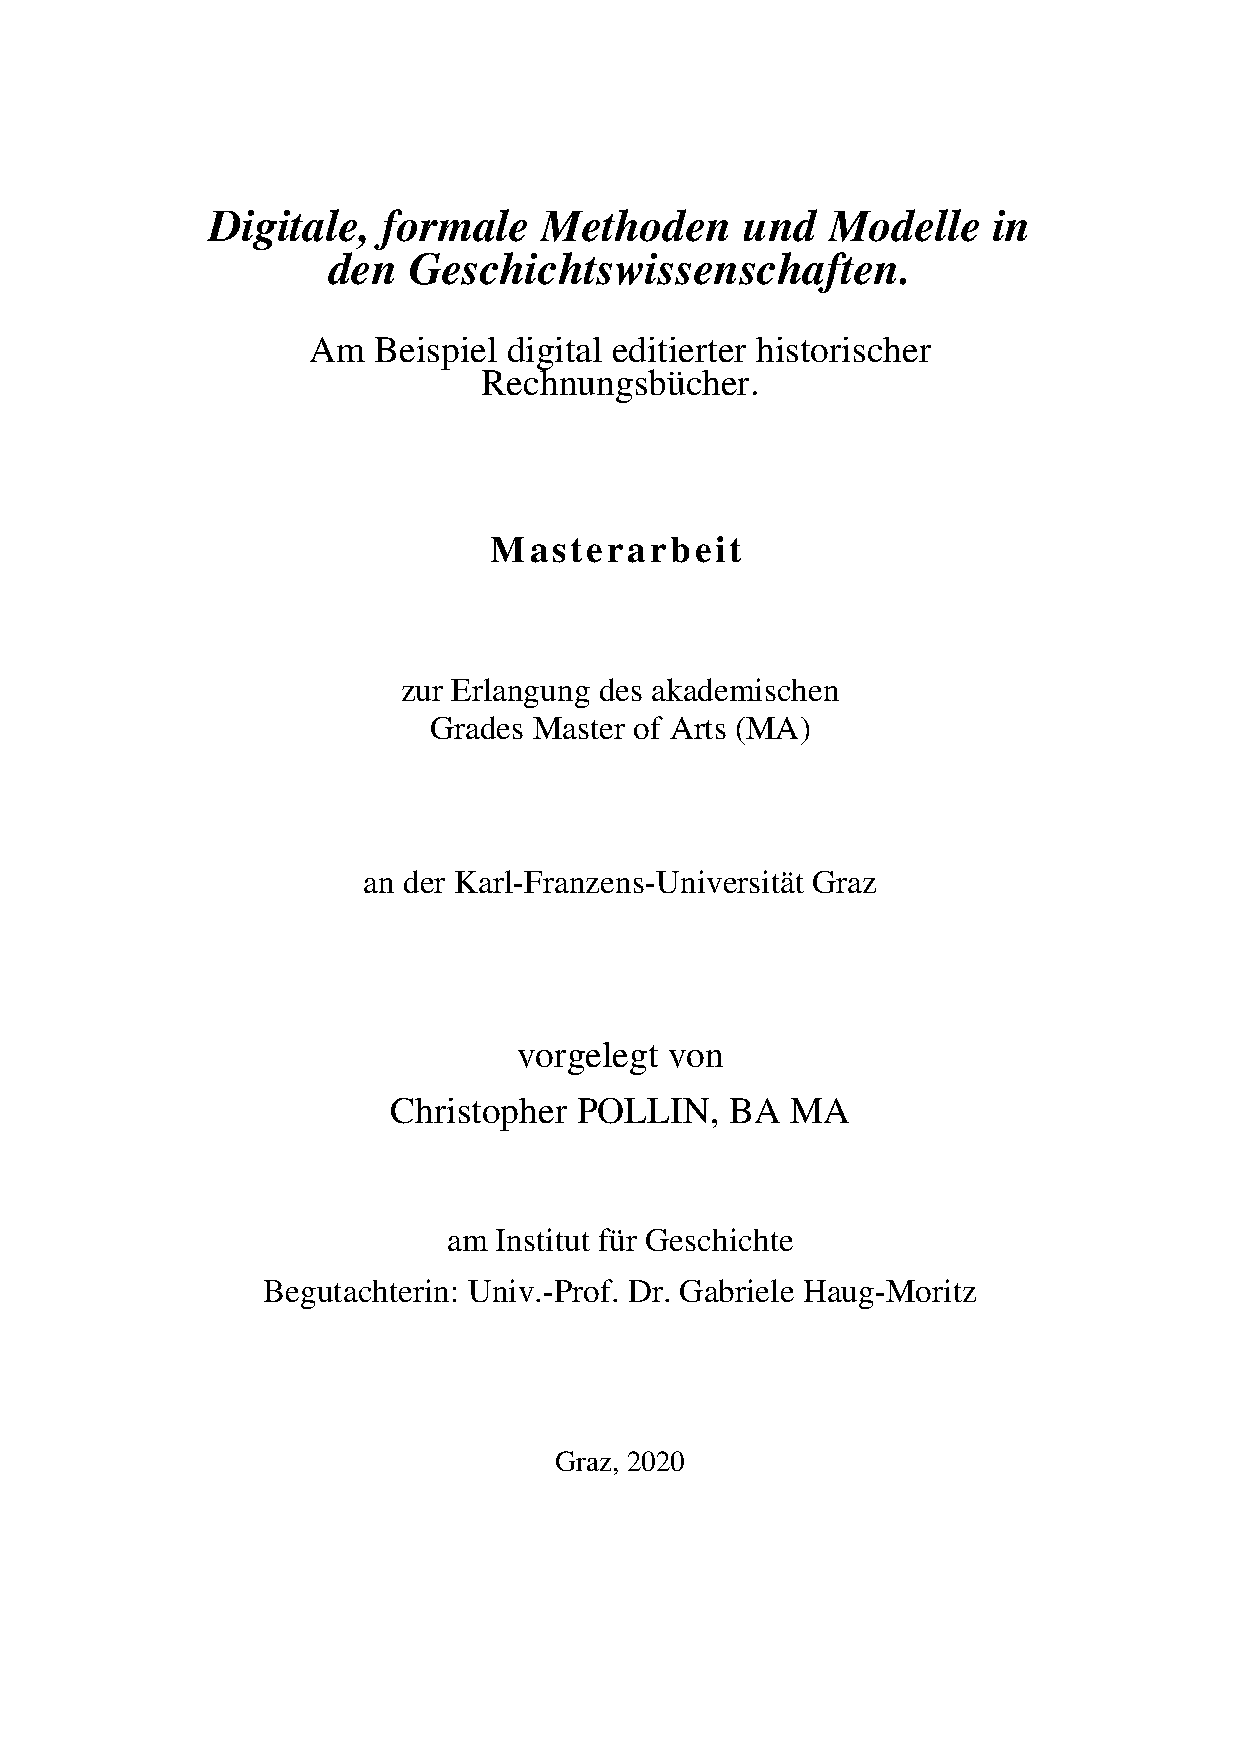
\includepdf[pages=-,pagecommand={}]{Deckplatt.pdf}
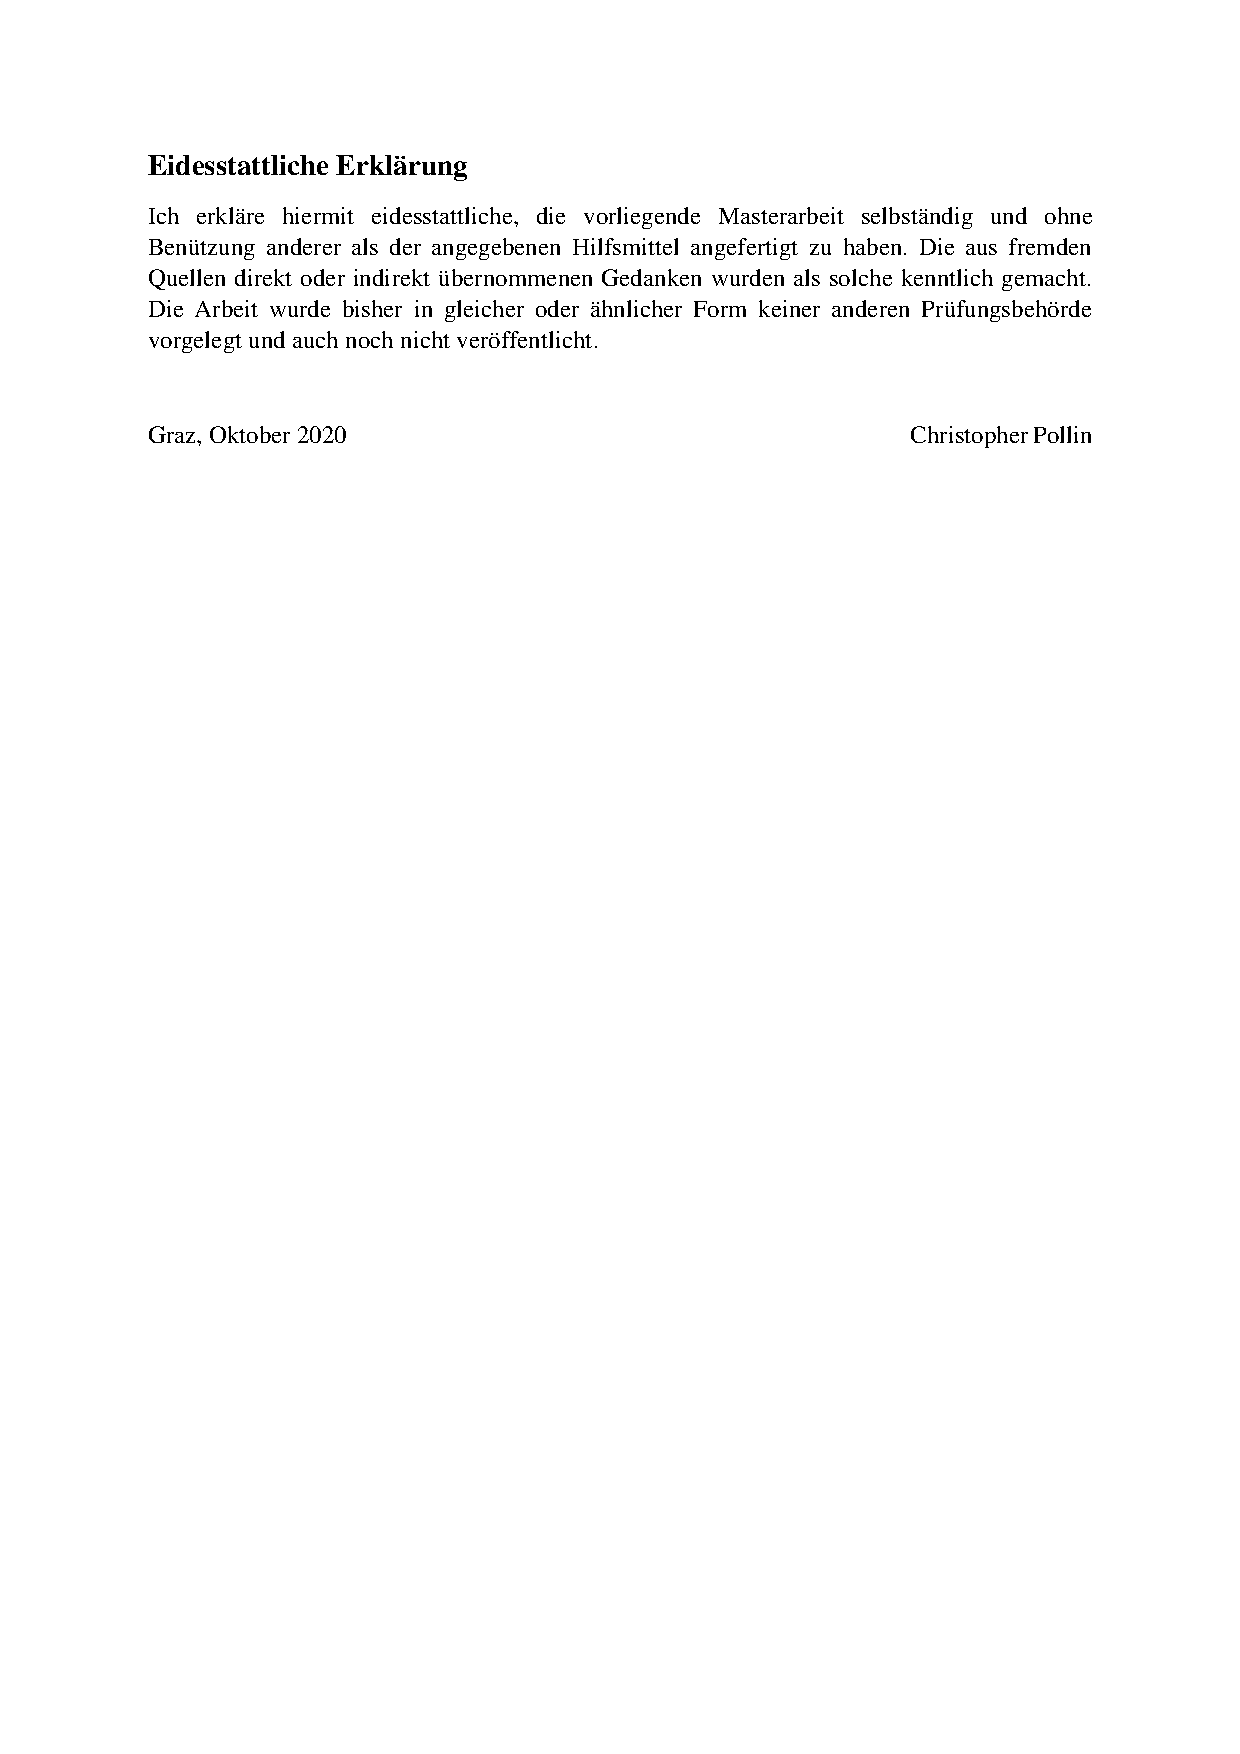
\includepdf[pages=-,pagecommand={}]{Erklarung.pdf}
\tableofcontents

\newpage
\pagenumbering{arabic}

\section{Einleitung}

Seitdem Menschen sich an Ereignisse oder Erkenntnisse, die für sie wichtig waren, erinnern, existieren auch Formen dieses Wissen zu repräsentieren und zu speichern. Bereits in den ersten Hochkulturen schrieb man nieder, dass jemand bei jemand anderen in der Schuld stand. Bereits um 3000 v. Chr. lässt sich auf Tontafel finden: ''\textit{Alok schuldet dem Sumar 10 Eimer Korn}''.
Die Dokumentation ökonomischer Abhängigkeiten zwischen Akteuren stellt eine der ersten Formen dar, wie Wissen verschriftlicht und strukturiert wurde.\footcite[][]{robson1992accounting} Für Historiker*innen liefert diese Zeile ein Indiz auf ein vergangenes Ereignis. Wird es in einen bestimmten historischen Kontext gestellt, so lassen sich Forschungsfragen in den Geschichtswissenschaften formulieren, die dabei helfen, ein Ereignis aus der Vergangenheit zu rekonstruieren und auf diese Weise etwas über die Vergangenheit lernen zu können. Dabei können semantische Strukturen helfen, die innerhalb der schriftlichen Überlieferung -- der historischen Quelle -- stecken. Im Falle von ökonomischen Abhängigkeiten und Transaktionen lässt sich eine ''natürliche'' Struktur festmachen, die über die Kulturen und Gesellschaften, sowie Zeiten und geographische Räume vergleichbar ist. Dies gilt für eine Tontafel aus Mesopotamien, einer Abgabenliste einer europäischen Stadt im Mittelalter, einem privaten Rechnungsbuch eines Geschäftsmannes aus dem 19. Jahrhundert in den Vereinigten Staaten von Amerika, sowie für einen Rechnungsbeleg aus heutiger Zeit. Akteure schulden oder transferieren wirtschaftliche Güter oder Geldbeträge an andere Akteure.
\\
Die Beschreibung einer solchen semantischen Struktur kann durch ein konzeptuelles Modell erfolgen. Die Anwendung formaler Methoden unter Berücksichtigung eines solchen Modells, kann als Grundlage dafür dienen, Interpretationen der Vergangenheit -- ''\textit{wie es den gewesen sein könnte}''\footcite[][S.159]{thaller2017ungefahre} -- mit einer gewissen Datengrundlage zu untermauern. Auf dieser Datengrundlage, die stets offen und nachvollziehbar, sowie in die fachwissenschaftliche Diskussion eingebettet sein muss und deswegen ein konzeptuelles Modell benötigt,  können die Interpretationen der Historiker*innen fußen. Die Rekonstruktion, Interpretation und die Einbindung dieser Erkenntnisse in gegenwärtige Diskussion ist die eigentliche Arbeit der Geschichtswissenschaft.
\\

Ziel dieser Arbeit ist eine theoretische und pragmatische Auseinandersetzung mit den Herausforderungen und Möglichkeiten, die formale -- und somit auch digitale -- Methoden und Modelle in der Geschichtswissenschaft mit sich bringen. Der praktische Anteil dieser Arbeit bezieht sich auf die Anwendung formaler Methoden auf semantisch angereicherte digitale Editionen von historischen Rechnungsbüchern in einem konkreten Projektkontext. Dieser Projektkontext -- \textit{Digital Edition Publishing Cooperative for Historical Accounts} (DEPCHA)\footnote{NHPRC-Mellon Implementation Grants: Digital Edition Publishing Cooperatives, \url{archives.gov/nhprc/announcement/depc}. Finanziert durch The Andrew W. Mellon Foundation \url{ mellon.org} 05.06.2019.} -- umfasst eine Kooperation von Partnern aus der USA, koordiniert durch das \textit{Wheaton College Massachusetts}, dem \textit{Center for Digital Editing} der University of Virginia und dem \textit{Zentrum für Informationsmodellierung} (ZIM) der Universität Graz. Es setzt sich zum Ziel eine Publikationsplattform für digitale Editionen historischer Rechnungsbücher zu entwickeln und umzusetzen. Eine Herausforderung in diesem Projekt umfasst die Diskussion und Zusammenführung quantitativer und qualitativer Herangehensweisen von Historiker*innen an Forschungsfragen in den Geschichtswissenschaften. Einen zentralen Stellenwert darin hat die sogenannte \textit{Bookkeeping Ontology}, die als konzeptuelles Modell die semantische Struktur von Rechnungsunterlagen beschreibt und im Sinn des \textit{Web of Data} (aka. Semantic Web) implementiert ist.
\\
\\
Diese Arbeit geht nun folgern Forschungsfrage nach:
\\
\\
\textcolor{red}{
\textbf{Inwieweit können Technologien des \textit{Web of Data} genutzt werden, um geschichtswissenschaftliche Fachdomänen, in diesem Fall die Edition und Analyse von historischen Rechnungsbücher, so zu beschreiben, dass die Anwendung formaler Methoden den geschichtswissenschaftlichen Kriterien gerecht wird und die Zurverfügungstellung als hochstrukturierte Forschungsdaten, sowie Formen der Analyse (z.B. Informationsvisualisierung), die weitere Interpretation von Forschungsfragen verbessert?} 
}

\subsection{Aufbau der Arbeit und Literaturübersicht}
Am Anfang der Arbeit steht neben einer allgemeinen theoretischen Diskussion zu Theorien und Methoden in den Geschichtswissenschaften\footcite{jordan2018theorien}\footcite{hardtwig1990geschichtskultur} eine Auseinandersetzung mit der Anwendung formaler Methoden in diesem Fachbereich\footcite{thaller2017ungefahre} unter Einbeziehung von Inhalten aus dem Bereich der historischen Fachinformatik\footcite{thaller2017historical}, der digitalen Geisteswissenschaften\footcite{jannidis2017digital} und Digital History\footcite{graham2015exploring}. Ziel ist es, einen Überblick darüber zu verschaffen, welche Ziele die Geschichtswissenschaft verfolgt. Dabei wird besonders Rücksicht auf die ''digitale'' Komponente\footcite{fohr2017historische}\footcite{wintergrun2019netzwerkanalysen} in diesem Zusammenhang genommen, um zu zeigen, dass es keine Gegensätze zwischen ''analoger'' und ''digitaler'' Geschichtswissenschaft gibt, sondern Synergien.
\\
\\
Das nächste Kapitel versteht sich als Quellenstudie und behandelt den Quellentypus historischer Rechnungsbücher\footcite{gleba2015wirtschafts} und ihre Edition\footcite{vogeler2015mittelalterliche}. In einem zweiten Schritt werden konkrete Editionsprojekte aus DEPCHA angeführt. Diese Auswahl umfasst drei Projekte, die \textit{George Washington’s Financial Papers}\footnote{The George Washington Financial Papers Project, \url{financial.gwpapers.org}, 30.01.2020.}, die \textit{Wheaton Family Papers}\footnote{Wheaton Family Papers, \url{digitalrepository.wheatoncollege.edu/handle/11040/7928}, 30.01.2020.} und die \textit{Stagville Accounts}\footnote{Stagville Accounts, \url{fromthepage.com/agbedavies/stagville-accounts}, 30.01.2020.}.
\\
\\
Eine Möglichkeit Modelle\footcite[][]{stachowiak1973allgemeine}\footcite{mccarty2004modeling} zu implementieren, ist mit den Standards des \textit{Web of Data} gegeben. Im vierten Kapitel wird auf den Technologie Stack des \textit{Web of Data} eingegangen und so die Grundlage zur konzeptuellen und daraus abgeleiteten formalen Beschreibung von Information im \textit{World Wide Web} erörtert. Dazu ist eine konzeptionelle\footcite{berners2001semantic}, technische\footcite{bernstein2016new} und kritische\footcite{swartz2013aaron} Diskussion dieses Themenbereiches notwendig. Ein zentraler Aspekt dabei sind die Themen Ontologien\footcite{stuckenschmidt2009ontologien} und \textit{Linked Open Data}\footcite{bauer2011linked}, die dazu dienen können Modelle und Forschungsdaten\footcite{neher2011semantische} über das Web auszutauschen.
\\
\\
Der gemeinsame Nenner dieser Projekte umfasst neben der zeitlichen und regionalen Einordnung der Quellen, auch den methodische Zugang der Erschließung. Diese erfolgt im Sinne einer digitalen Edition\footcite{sahle2013digitale}. Der dabei verwendete Standard ist die \textit{Text Encoding Initiative (TEI)}\footcite{cummings2013text}. Dieses Kapitel widmet sich der Fragestellung, wie digitale Edition von historischen Rechnungsbüchern umgesetzt werden können\footcite{tomasek2013encoding}\footcite{vogeler2016content} Die digitale Edition in dieser Arbeit versteht sich als quellen-orientierte und inhaltsbezogene Edition, in der nicht jedes textuelle Phänomen ediert werden muss, sondern die semantische Struktur der Quellen im Vordergrund stehen.\footcite{vogeler2019assertive} Zur formalen Beschreibung semantischer Strukturen kann das \textit{Web of Data} herangezogen werden. Dies soll am Beispiel der \textit{Bookkeeping Ontology}\footcite{pollin2019digital}, einem konzeptuellen Modell zur Beschreibung von Transaktionsprozessen in historischen Rechnungsunterlagen, diskutiert und reflektiert werden. Auf diesem Modell und den Forschungsdaten werden weiter formale Methoden zur Analyse von Rechnungsbüchern im Sinne einer Informationsvisualisierung\footcite{preim2010interaktive} beschrieben und reflektiert.

%%%%%%%%%%%%%%%
\subsection{Related Work}

Es lässt sich eine Vielzahl von Projekten festmachen, die quantitative, formale und/oder digitale Verfahren zur Bearbeitung und Erschließung von historischen Quellen verwenden und darüber reflektieren. Dabei gibt es auch zahlreiche Beispiele hinsichtlich des Quellentypus der historischen Rechnungsbücher, der digitaler Edition dieser Quellengattung, sowie der Anwendung von \textit{Web of Data} Technologien im Bereich der Geisteswissenschaften.
\\
\\
VASOLD hat in seiner Arbeit in den 1990er Jahren mit der computergestützten Verarbeitung der Itinerar\footnote{Als Itinerar versteht man nicht nur Reiseberichte, sondern auch die Methode der Rekonstruktion der getätigten Wege einer Person oder Gruppe.} des Erzbischofs Konrad IV. von Salzburg die Möglichkeiten und den Mehrwert formaler Methoden in den Geschichtswissenschaften gezeigt. Er hat auf Basis eines mittelgroßen Quellenbestandes aus Urkunden und historiographischen Belegen, die Reisetätigkeiten eines Erzbischofes aus dem Mittelalter rekonstruiert, in dem er ein Modell zur formalen Beschreibung der gesammelten Belege entwickelt und die Daten daraus im quellenorientierten Datenbanksystem Kleio verarbeitet hat. Kleio ist ein Datenverarbeitungsprogramm, aus den 80iger und 90iger Jahren, das die Arbeit von Historiker*innen unterstützt und die Arbeit mit komplexen (historischen) Daten ermöglicht.\footcite[][S.172-174]{hoffmann1990ehepaare}  Als Vorteil dieser Herangehensweise führt VASOLD an, dass durch die Ein- und Ausblendung bestimmter Strukturen und Quellen, sich ein stabiles Bild des Weges einer Person skizzieren lässt.\footcite{vasold1996itinerar}
\\
\\
Unter Verwendung der ''\textit{dynamisch integierten computergestützten Edition}'' hat PERSTLING das Steirische Marchfutterurbar aus den Jahren 1412 bis 1426 so erschlossen, dass unterschiedliche Bearbeitungsschichten des Dokuments als digitale Edition über das Web nachvollziehbar werden.\footcite{PerstlingMatthias2013MDuE} So wird das Fundament für künftige  Erforschungen von beispielsweise Preisen, Münzen oder prosopographischen\footnote{Bezeichnet in der Geschichtswissenschaft die systematische Erforschung eines bestimmten Personenkreises.}, wie  auch onomastischen\footnote{Bezeichnet die Namensforschung, die die Verbreitung, Bedeutung und Herkunft von Eigennamen erforscht.} Studien gelegt.
\\
\\
BURGHARTZ, CALVI und VOGELER haben eine TEI/XML basierte digitale Edition des Basler Urfehdebuchs X, das Urfehedeeinträge aus den Jahren 1563 bis 1569 beinhaltet, im Web veröffentlicht. Als Urfehde versteht man ein Rechtsmittel in der Neuzeit, um einen Konflikt zweier Parteien zu schlichten. Die digitale Edition liefert eine transkribierte Quelle, die nach einem konzeptuellen Modell semantisch beschrieben wurde. Täter, Tat, Opfer, Strafen und personenbezogene Information werden so maschinenlesbar strukturiert und können weiter ausgewertet werden.\footcite[][S.27-29]{pollin2017semantically} 
\\
\\
Ein weiteres Beispiel für die Zurverfügungstellung eines administrativen, historischen Quellenkorporus über das Web ist das \textit{Itinera Nova} Projekt. Das Stadtarchiv Leuven hat in Kooperation mit dem \textit{Cologne Center for eHumanities} und dem \textit{Data Center for the Humanities} der Universität Köln 950.000 Seiten aus Schöffenakten aus der Zeit zwischen 1362-1795 digitalisiert und im Volltext indiziert.\footnote{Itinera Nova - Redaktions- und Präsentationssystem für die mittelalterlichen Schöffenakten der Stadt Leuven, \url{itineranova.be}, 30.01.2020.}
\\
\\
Da Rechnungsbüchern eine relativ einheitliche und ''natürliche'' Struktur aufweisen und ihr Inhalt sich für die Anwendung quantitativer und computergestützter Methoden eignet, lassen sich eine Vielzahl von Projekten festmachen, die Rechnungsunterlagen formal ausgewertet haben. Hier sind nur einige wenige angeführt:
\\
\\
Im Projekt ''\textit{Rechnungsbücher von Bistritz aus den Jahren 1461–1520 ediert}'', werden Steuerverzeichnisse erschlossen, die einen Einblick in die wirtschaftliche und soziale Struktur der drittgrößten Stadt Siebenbürgens zu dieser Zeit liefern.\footnote{Rechnungsbücher von Bistritz aus den Jahren 1461–1520 ediert, \url{tinyurl.com/rgxw27q}, 15.07.2019}
\\
\\
In einer anderen Kooperation haben BURGHARTZ und VOGELER die ''\textit{Jahrrechnungen der Stadt Basel}'' in den Jahren 1535 bis 1610 digital ediert und im Web veröffentlicht. Jedes Rechnungsbuch beschreibt Einkünfte und Ausgaben der Stadt Basel, wie beispielsweise Einnahmen durch das \textit{Weinungeld}, einer Abgabe an die Stadt, die durch den Ausschank von Wein fällig wurde. Die digitale Edition verfügt über Funktionalitäten einzelne Einträge zu sammeln und  Berechnungen damit anzustellen.\footcite[][S.11-13, \protect\url{gams.uni-graz.at/srbas}]{vogeler2016content}
\\
\\
''\textit{Die digitale Edition der Augsburger Baumeisterbücher}''\footnote{Die Augsburger Baumeisterbücher. Digitale Edition der mittelalterlichen Stadtrechnungen von 1320 bis 1466 \protect\url{augsburger-baumeisterbuecher.de}}, erlaubt den Zugang zu XML-basierten Transkriptionen der Quellen. Sowohl Digitalisate, wie auch Indices zu Personennamen, Orten und Schlagwörtern sind im Web aufrufbar und durchsuchbar. Eine Normalisierung von Namensformen beispielsweise wird über die GND\footnote{Gemeinsame Normdatei, \protect\url{dnb.de/DE/Professionell/Standardisierung/GND/gnd_node.html}} sichergestellt.\footcite[][S.109-113]{wurz2016dh}
\\
\\
NEUWÖHNER beschreibt ausführlich eine Geschichte der Stadt Paderborn im 17. Jahrhundert, die auf den Einnahmen und Ausgaben der Stadtrechnungen basiert. Nicht die Erfassung und Edition der historischen Quellen liegt in dieser Arbeit im Vordergrund, sondern veranschaulicht sie, wie reichhaltig die geschichtswissenschaftliche Interpretation des Quellentypus Stadtrechnung sein kann, um die finanzielle, wirtschaftliche und soziale Dimension einer Stadt zu erforschen.\footcite[][S.11-50]{neuwohner2016rechnen}  
\\
\\
Zuletzt sei die Arbeit von ZIEGLER angeführt, die zwar nicht digital ist, aber zeigt, dass die Überlegungen zur Anwendung quantitativer Methoden auf historische Rechnungsbücher dazu führen kann, komplexere Sachverhalte zu bearbeiten, wie etwa den Staatshaushalt Bayerns in der zweiten Hälfte des 15. Jahrhunderts. In seiner Zusammenfassung ist sich ZIEGLER bewusst, dass auf Grund der unscharfen und lückenhaften Datengrundlage es sich nur um eine historische Annäherung handeln kann, die aber dennoch für die Geschichtswissenschaften relevant sind.\footcite[][S.221-230]{ziegler1981Staatshaushalt}

\newpage
%%%%%%%%%%%%%%%%%%%%%%%%%%%%%%%%%%%%%%%%%%%%%
%%%%%%%%%%%%%%%%%%%%%%%%%%%%%%%%%%%%%%%%%%%%%
\section{Formale Methoden und Modelle in den Geschichtswissenschaften}

Am ersten August des Jahres 1808 hat ein gewisser \textit{James Haley} 1/4 Pfund Pulver, 1 Pfund Munition und 1 Pfund Zucker zum Preis von 2 Schilling und 6 Pence im Laden der \textit{Stagville Plantage} in \textit{North Carolina} käuflich erworben. Diese Art von Information über die Vergangenheit lässt sich in historischen Rechnungsbüchern finden. Dabei ist nicht der Einzeleintrag von großer Bedeutung für Fragestellungen in den Geschichtswissenschaften, sondern die Aggregation vieler Einzelinformationen, um eine Datengrundlage zu schaffen, auf der eine weitere fachwissenschaftliche Auseinandersetzung -- eine Interpretation der Vergangenheit -- durch Historiker*innen fußt.\footcite[][06.06.2019]{vogeler2015mittelalterliche}
\\
Damit diese Datengrundlage ausreichend groß ist und Aussagen nicht nur auf Ausschnitte eines Quellenkorpus reduziert sind, ist es notwendig, formale Verfahren zur Erschließung, Veröffentlichung und Analyse zu verwenden. Auf historische Rechnungsbücher bezogen, können so Berechnungen angestellt werden, die zeigen, wie sich etwa der Preis einer Ware über eine bestimmte Zeitspanne entwickelt hat, oder welche Waren von welchen Akteuren gekauft und verkauft werden. Die Menge an unterschiedlichen Fragestellungen ist groß und wird in Kapitel drei weiter veranschaulicht. Setzt man diese ''historischen Fakten'' aus der Quelle in einen größerer historischen Zusammenhang und als Diskussionsbeitrag in die fachwissenschaftliche Diskussion, beginnt die ''klassische'' Arbeit von Historiker*innen. 
\\
Im Mittelpunkt dieses Kapitels steht eine Diskussion über \textbf{Theorien und Methoden der Geschichtswissenschaften} und einer darauf aufbauenden Auseinandersetzung mit der Entwicklung der Anwendung formaler Verfahren innerhalb des Faches. Es wird der Frage nachgegangen, welche theoretischen und methodischen Herangehensweisen sich in den Geschichtswissenschaften etabliert haben. So stellt sich beispielsweise die Frage was man als ''historische Fakten'' verstehen kann und wie man sie nachvollziehbar, ohne die Quellen zu verzerren, algorithmisch verarbeiten kann. Bereits in den 1980er Jahren hat man sich im Fachbereich \textit{Historische Fachinformatik} mit diesen Fragen beschäftigt.
\\
Getrieben von einer analytischen Geschichtswissenschaft, in der die Theoriebildung ein zentrales Moment ist, wird die Anwendung formaler und computergestützter Verfahren zur Verarbeitung von Quellen und eine methodische Diskussion darüber immer wichtiger. Aus den Sozialwissenschaften kommend, in der \textbf{Historischen Fachinformatik} im Selbstverständnis einer Hilfswissenschaft weiterentwickelt, erleben formale Methoden eine neue Renaissance. Die \textbf{Digital Humanities} und die \textbf{Digital History} sind zwei Begriffe die dafür stehen. Ein Kernaspekt dieser fachlichen Ausrichtungen ist die Erarbeitung und Anwendung von Modellen, um \textbf{historische Forschungsdaten} sinnvoll in eine nutzbare  Struktur überführen zu können. So setzt sich dieses Kapitel auch mit einer grundlegenden Erörterung der \textbf{Modelltheorie} und Modellbildung in den Geisteswissenschaften bzw. Geschichtswissenschaften auseinander.

\subsection{Von der erzählenden zur theorieorientierten Geschichtswissenschaft}

''\textit{Ich glaube an diese ganze Theoriebedürftigkeit der Geschichte nicht. Die Historie ist eine Kunst, die auf Kenntnissen beruht, und weiter ist sie gar nichts'}'\footcite[][S.53]{mann1979pladoyer}
\\
\\
Führte MANN im Jahr 1979 an, um auszudrücken, dass durch die Einführung damals neuartiger, theoretischer Ansätze die Hauptaufgabe der Geschichtswissenschaften --  das Erzählen von Geschichten -- aufgeweicht wird. Bereits in den 1960er Jahren forderten Historiker wie MOMMSEN, KOCKA oder WEHLER eine ''\textit{Reform der Geschichtswissenschaft jenseits des Historismus}'' hin zu einer analytischen und theorieorientierten Geschichtswissenschaft. Ihre Kritik richtet sich an den individualistischen Ansatz des Historismus, der Geschichte als Produkt menschlichen Handelns und nicht als rationales Ergebnis eines gesellschaftlichen Prozesses versteht. Die Kritik richtet sich explizit an dieses zentrale Element des Historismus. Die Errungenschaften der historisch-kritischen Methode, der Quellennähe und der Verwissenschaftlichung des Faches, \textcolor{red}{die sich als ''historische Betrachtung'' als allgemeines Paradigma der Geistes- bzw. Kulturwissenschaften durchsetzte\footcite[][S.28]{hardtwig1990geschichtskultur},} werden stets positiv hervorgehoben. Sie fordern eine stärkere Theoriebildung in der Geschichtswissenschaft und orientieren sich mehr und mehr an der Methodik der benachbarten Sozialwissenschaften, wie etwa der Soziologie. Die reine Nacherzählung der Vergangenheit, wie sie MANN noch einforderte, ist im heutigen Verständnis der Geschichtswissenschaft, ohne Anbindung an jegliche theoretische Fragestellungen, nicht mehr denkbar.
\\
Heutzutage ist die Orientierung an Theorien in den Geschichtswissenschaften wichtiger Bestandteil. KOCKA versteht darunter einen expliziten Gebrauch von Modellen, Theorien und Begriffen zur Strukturierung des Gegenstandes.\footcite[][S.2]{magerski2009schreibt} Je stärker man sich beispielsweise mit historischen Fragestellungen, die soziale oder wirtschaftliche Phänomene untersuchen, wie die Beziehungen zwischen sozialen Klassen oder öknomisches Wachstum, steigt auch die Notwendigkeit mehr über die Fragestellungen und Theorien der Sozial- und Wirtschaftswissenschaft zu wissen.\footcite[][S.6-8]{kocka1982theorien} So ist ein grundlegendes Verständnis über Modelle der Konjunkturtheorie oder klassentheoretische Konzepte der Sozialgeschichte unabdingbar.\footcite[][S.1]{sokollgrundlagen}
\\
Der vermehrte Einsatz formaler Verfahren zur Erschließung, Auswertung und Darstellung von Information in historischen Quellen, befördert diese Notwendigkeit.

%%%%%%%%%%%%%%%%%%%%%%%%%%%%%%%%%%%%%%%%%%%%%
\subsubsection{Geschichte und Geschichtswissenschaft: eine Definition}
Gegenstandsbereich der \textbf{Geschichte} ist das Handeln der Menschen in der Vergangenheit. Dieses Handeln ist aber für niemanden mehr erlebbar, sondern muss über Belege der Vergangenheit, den Quellen, ob als Überrest oder Tradition, rekonstruiert werden. Die Unterscheidung erfolgt nach DROYSEN zwischen ''unabsichtlich'' erzeugten Überresten, wie etwa ein Kleidungsstück, das bei einer archäologischen Ausgrabung gefunden wurde, und absichtlich überlieferten Quellen, wie etwa ein Denkmal. Letztere werden als Tradition verstanden.\footcite[][49–55]{schulz2010neuere} Bei dieser Einteilung handelt es sich aber um ein Ideal, da für eine genaue Zuordnung das Wissen über die Intention der Schöpfer notwendig wäre. 
\\
\\
KIRN führt in seinem Einführungswerk in die Geschichtswissenschaft mehrere Definitionen des Begriffes Geschichte an. Wo HELLPACH über ''\textit{die bewußte Gestaltung menschlichen Gemeinschaftslebens aus schöpferischem Willen}'' spricht und die menschliche Handlung in den Vordergrund stellt, ist es für HUIZINGA, aus dem Verständnis von Geschichtswissenschaft als Kulturgeschichte, ''\textit{die geistige Form, in der sich eine Kultur über ihre Vergangenheit Rechenschaft gibt}''. Zentral in dieser Menge an Definitionen und Zugängen zur Geschichte ist, dass es sich um die wissenschaftliche Darstellung des Vergangenen handelt.\footcite[][S.7-12]{KirnPaul2015EidG} Zweiter zentraler Aspekt ist, dass der Mensch als gesellschaftliches und kulturelles Wesen etwas über sich selbst, seine vergangenen Gesellschaft- und Kulturformen wissen möchte. Man könnte es als einen Akt der kollektiven Selbstreflexion verstehen. Jedenfalls ist der Begriff mehrdeutig. Geschichte kann als Vergangenheit, Geschichtsforschung oder Geschichtsschreibung verstanden werden. Geschichtsschreibung als Produkt der Geschichtsforschung liegt üblicherweise als Narrativ über vergangene Ereignisse vor. Sie ist jedoch nicht auf die Textform beschränkt, sondern kann auch in anderer Form vorliegen. Dies umfasst mündliche, wie bildliche Überlieferungen oder sämtliche Schöpfungen, die von Menschen erbracht wurden, um in einen Kommunikationsprozess einzutreten.\footcite[][S.5-7]{frank2018visualisierungswerkzeuge}
\\
\\
Bei DEMANDT finden sich weitere Ausführungen zu den grundlegenden Überlegungen des Begriffes \textit{Geschichte}. Neben dem Mythos, der in vorschriftlichen Zeiten und in erzählerischer Form Vergangenes von einer Generation zu anderen weitergibt, war die Chronistik eine früher Form der verschriftlichten Erinnerung. Chroniken berichten über Ereignisse, ohne die Texte literarisch aufzuarbeiten. Die \textbf{Historie}, die \textit{Erkundung der Vergangenheit}, geht noch einen Schritt weiter und versucht Ereigniszusammenhänge einer ''wahren'' Vergangenheit darzustellen. \textcolor{red}{Sie etabliert sich als autonome Disziplin, die mehr den Wandel der Geschichte und das Geschehene an sich versucht zu erklären, denn moralisch und belehrend auf Rezipierende zu wirken, wie es die Geschichtsüberlieferung davor getan hat.\footcite[][S.24]{hardtwig1990geschichtskultur}}
\\
Im 16. Jahrhundert entwickelt sich der Begriff Geschichte, der anfangs nur für den Gegenstandsbereich der Historie verwendet wurde.\footcite[][S.57-58]{schulz2010neuere} \textcolor{red}{Mit diesem Verständnis geht auch einher, dass das was als Gegenwart verstanden wird, sich von der Vergangenheit unterscheidet, aber von ihr bedingt ist. So fasst ein Zitat von SCHILLER dieses neue Paradigma der Geschichtswissenschaft zusammen, welches bis heute gilt: “\textit{Das Verhältnis eines historischen Datums zu der heutigen Weltverfassung ist es also, worauf gesehen werden muss}”. Geschichtswissenschaft, ist erst dann vollkommen, wenn sie mit der Gegenwart in Beziehung gesetzt wird und umgekehrt.\footcite[][S.25]{hardtwig1990geschichtskultur}
}
\\
\\
Das moderne Verständnis des Wortes Geschichte umfasst sowohl die Gesamtheit von realen Geschehnissen, als auch den Bericht und die Reflexion darüber. Zentral in der \textbf{modernen Geschichtswissenschaft}, also der Erforschung der Vergangenheit nach wissenschaftlichen Kriterien, ist die Auseinandersetzung mit historischen Quellen, die mittels kritischer Methode untersucht werden. In diesem Prozess müssen die angewandten Methoden, Ideen und Ergebnisse diskutierbar und nachprüfbar sein.\footcite[][S.13-32]{demand2011philosophie} Jede und jeder soll in der Lage sein, feststellen zu können, ob eine Interpretation eines historischen Sachverhalts durch eine angeführten Quelle belegbar ist. Forschungsgegenstand und Forschungsfrage sind in den Geschichtswissenschaften nicht klar abgegrenzt und die Interessen von Historiker*innen sind interdisziplinär, weswegen auch die angewandte Methodik vielfältig ist.\footcite[][S.13]{reiche2014verfahren} Auf die Methoden in den Geschichtswissenschaften wird in Kapitel \ref{ref:Methoden} detaillierter eingegangen.
Zwei grundlegende Strömungen in der Erkenntnis- und Wissenschaftstheorie sind wichtig und werden im Folgenden weiter ausgeführt: die Hermeneutik und der Empirismus.


%%%%%%%%%%%%%%%%%%%%%%%%%%%%%%%%%%%%%%%%%%%%%
%%%%%%%%%%%%%%%%%%%%%%%%%%%%%%%%%%%%%%%%%%%%%
\subsubsection{Hermeneutik}

Bei der Hermeneutik handelt es sich um eine Theorie der Interpretation und des Verstehens von Texten, die nicht nur auf die Geschichtswissenschaft angewendet wird, sondern auf viele geisteswissenschaftliche oder rechtswissenschaftliche Fächer.
DILTHEY betont, ''\textit{dass das Verstehen [...] die spezifische Operation der Geisteswissen darstellt.}\footcite[][S.82]{ficara2015hermeneutik}
\\
Im großen Unterschied zu naturwissenschaftlichen Fragestellungen, ist die Vergangenheit nicht in einem Experiment beweis- bzw. widerlegbar. Geprägt wird die Hermeneutik, als Theorie für die Geschichtswissenschaften, unter anderen, von den Arbeiten von SCHLEIERMACHER, der sie zu einer \textit{universellen Theorie des Verstehens} weiterentwickelte, in der jedes Verstehen einen individuellen Prozess darstellt. Für SCHLEIERMACHER ist gerade die Sprache, als Ausdruck der Gedanken von Individuen wichtig.\footcite[][S.72-81]{ficara2015hermeneutik} 
\\
Aus dem neuen Geschichtsverständnis des 19. Jahrhunderts entwickelte DILTHEY die Hermeneutik zu einer historischen Methodik. Bei ihm wird Verstehen zur essentiellen Methode in den Geisteswissenschaften. Wo Naturwissenschaften die Welt von außen betrachten und gesetzmäßige Erkenntnis, beispielsweise durch das Zählen, Messen und der daraus ableitbaren Regeln, schließen, so ist die Aufgabe der Geisteswissenschaften, die Welt von innen zu verstehen.\footcite[][S.82-83]{ficara2015hermeneutik}
\\
Unter GADAMER wird die Hermeneutik zur Philosophie weiterentwickelt. Es bedarf immer einem Vorverständnis, um in einen Prozess des Verstehens eintauchen zu können, an dessen Ende nur eine Annäherung an eine Wahrheit möglich ist.\footcite[][S.19-30]{schulz2010neuere} Voraussetzung dafür ist die Frage nach der Anwendung und Konkretisierung der Fragestellung, die GADAMER als grundsätzliche Verwandtschaft von juristischer und hermeneutischer Rationalität beschreibt.\footcite[][S.176-178]{ficara2015hermeneutik}
\\
Nicht nur unser Wissen über historische Quellen, sondern alles Wissen beruht auf einem Verstehen, das in einer Auslegung unseres Wissens erläutert wird. Verstehen in diesem Sinne ist zirkelförmig. Jemand tritt mit einem gewissen Vorwissen an eine Fragestellung heran. Es werden in der Auseinandersetzung mit der Materie Erfahrungen gesammelt und ein tieferes Verständnis der Thematik erarbeitet. Mit diesem gefestigten Verständnis bewegt man sich im sogenannten  \textit{hermeneutischen Zirkel}, einem iterativen Prozess gleich, weiter fort und erhält auf diese Weise ein besseres Bild zu einem Thema. Eine Problemstellung muss zuerst gefunden, erkannt und verstanden werden, damit sie weiter verarbeitet werden kann.\footnote{STANGL, Werner: Geschichte der Hermeneutik, \protect\url{arbeitsblaetter.stangl-taller.at}, 01.06.2019.}
\\
\\
In folgendem Beispiel nach STANGL sind die Wörter ''\textit{vihe}'', ''\textit{verwürckt}'' oder ''\textit{fewer}'' ohne jeglichen Kontext unverständlich. Werden sie aber in ihrem Kontext gelesen, wird die Bedeutung des Textes offensichtlich:
\\
\\
"\textit{ltem so eyn mensch mit eynem vihe, mann mit mann, weib mit weib, vnkeusch treiben, die haben auch das leinen verwürckt, vnd man soll sie der gemeynen gewonheyt nach mit dem fewer vom leben zum todt richten}"\footnote{STANGL, Werner: Der hermeneutische Zirkel, \protect\url{arbeitsblaetter.stangl-taller.at}, 07.11.2019.}
\\
\\
Zentrale Begriffe lassen sich häufig erst aus dem Zusammenhang erschließen. Für das vollständige Verstehen des Gesamttextes müssen alle Einzelheiten nachvollziehbar sein. Die hermeneutische Spirale beinhaltet, dass Teilstücke ganzheitlich verstanden oder erweitert werden und sich das Ganze von den Teilaspekten her definieren lässt. Gerade in den Geschichtswissenschaften ist die Berücksichtigung und das Verstehen des Kontextes, in dem eine Aussage über die Vergangenheit steht, essentiell.
\\
Werden hermeneutischer Verfahren auf historisches Quellenmaterial angewendet, spricht man von einem historisches Verstehen, mit dem Ziel Geschichte und Vergangenheit in Relation zusetzen. Es ist der reflexive Prozess sich in einen Schöpfer einer geistigen Produktes, etwa einem historischen Rechnungsbuch, hineinzuversetzen. So sollen Erfahrungen, Denkweisen oder gar Gefühle reproduziert werden, um Handlungen in der Geschichte verständlich erscheinen zu lassen.\footcite[][S.14-20]{detel2011geist}


%%%%%%%%%%%%%%%%%%%%%%%%%%%%%%%%%%%%%%%%%%%%%
%%%%%%%%%%%%%%%%%%%%%%%%%%%%%%%%%%%%%%%%%%%%%

\subsubsection{Empirismus}

Wissenschaften, die Sachverhalte und Objekte der Welt durch Experimente im Labor, Beobachtung oder Befragung im Feld untersuchen, werden als empirische Wissenschaften zusammengefasst. Als sogenannte Erfahrungswissenschaft wird Erkenntnis aus der Erfahrung der Welt abgeleitet. Die klassischen Vertreter sind etwa die Disziplinen der Naturwissenschaften, wie die Physik oder Biologie. Die Mathematik, die Philosophie oder auch die Informatik wiederum sind keine empirischen Wissenschaften. In diesen Disziplinen findet keine direkte Beobachtung statt, sondern Aussagen basieren auf einer logischen bzw. formalen Herangehensweise.\footcite[08.11.2019]{frommergrundbegriffe} Abbildung \ref{fig:empirismus} zeigt die zentralen Begriffe der Empirie und ihre Wechselwirkung. Als Empirie wird die methodisch-systematische Sammlung von Daten verstanden, die zu einer Hypothese oder deren Widerlegung führt. Die \textbf{Deduktion} versteht die Schlussfolgerung gegebener Prämissen auf die logisch zwingenden Konsequenzen und die \textbf{Induktion} beschreibt den abstrahierenden Schluss aus beobachteten Phänomenen auf eine allgemeinere Erkenntnis.\footcite[Siehe][]{chalmers2007wege}
Oder anders formuliert: Schlussfolgerung vom Allgemeinen auf das Besondere und umgekehrt. Für die Geschichtswissenschaften bedeutet das ausgehend von einer Forschungsfrage verschaffen sich so Historiker*innen einen kritischen Überblick über  vorhandenes Quellenmaterial, entwickeln eine These und überprüfen diese anhand des Materials.\footcite[][S.45-46]{jordan2018theorien}
\begin{figure}[H]
\centering
	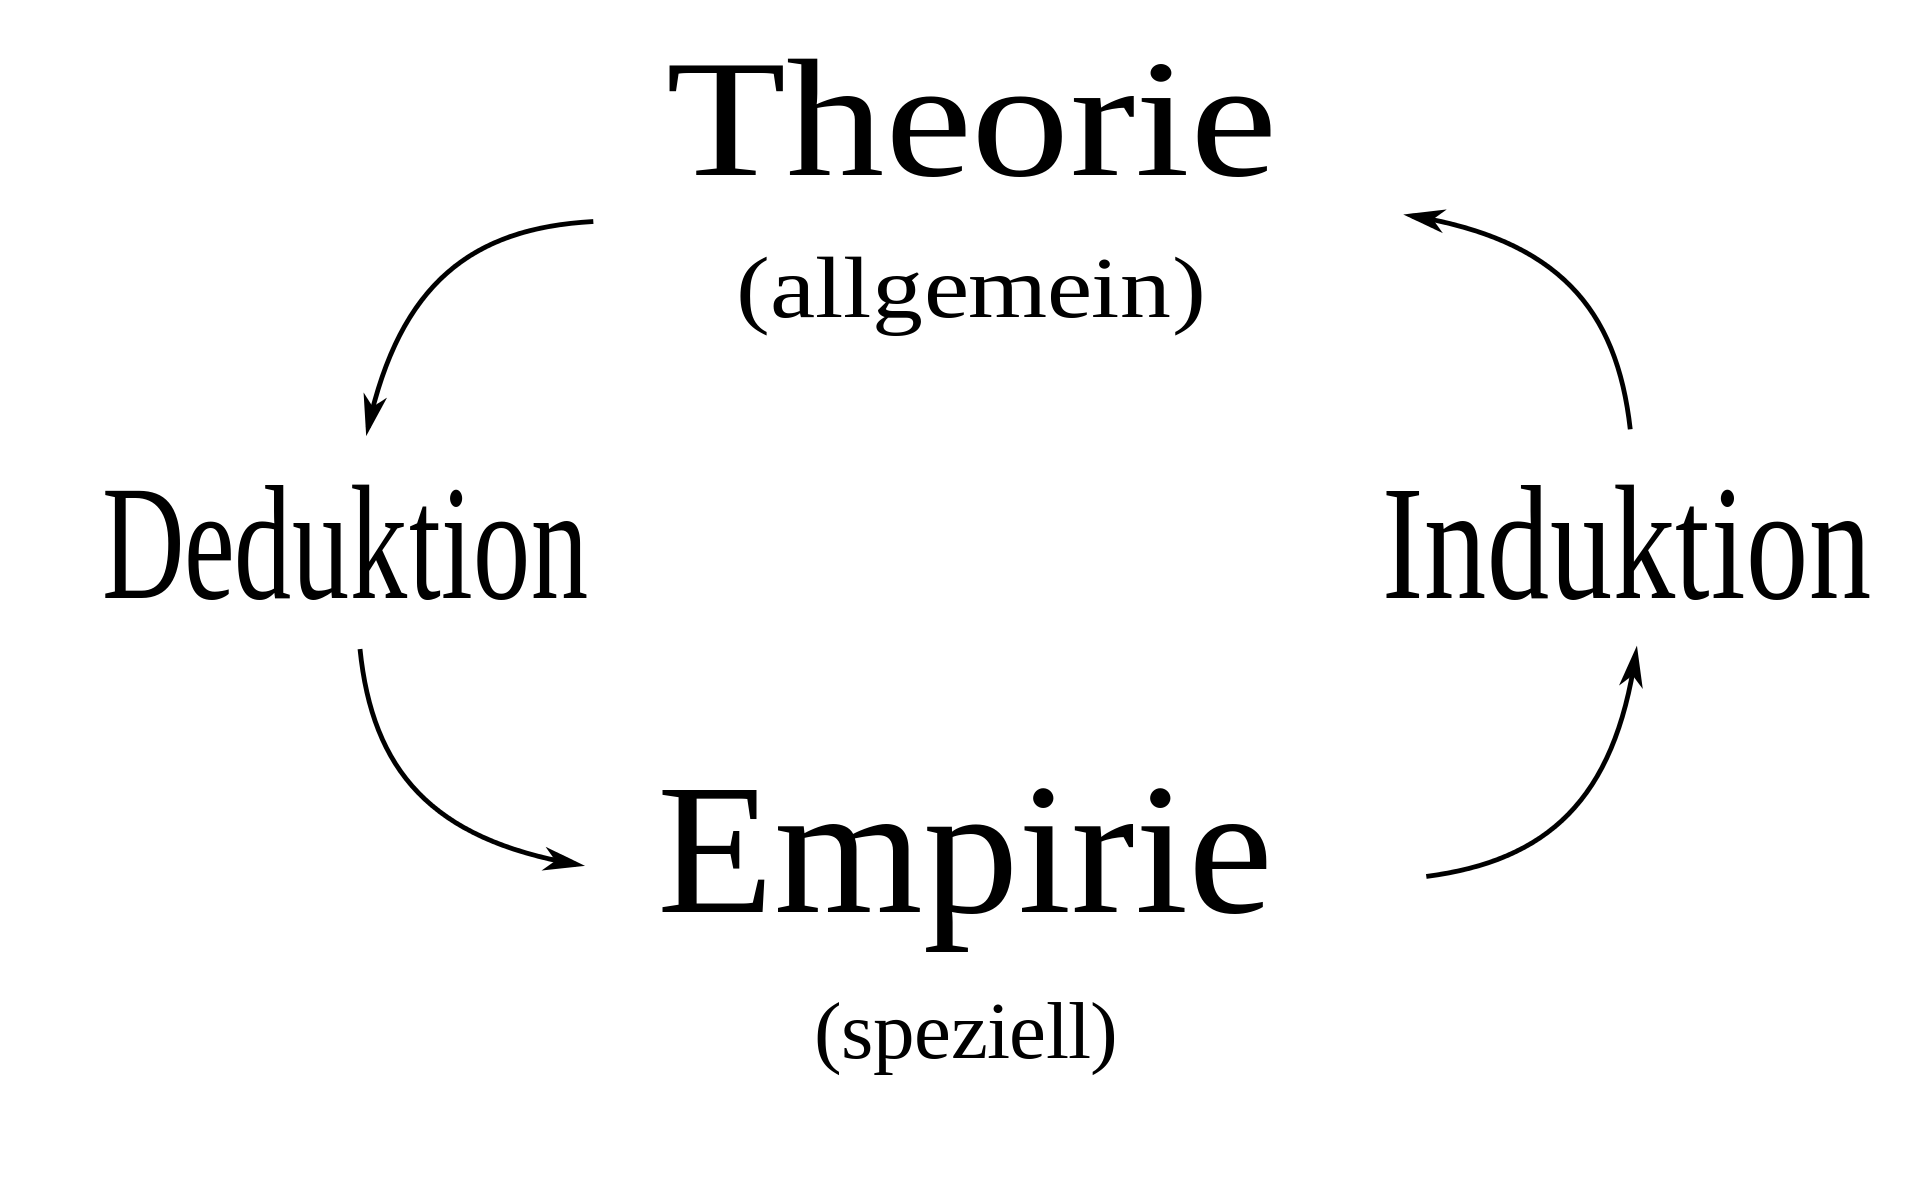
\includegraphics[width=0.85\textwidth]{img/emprisimus.png}  
    \caption[Zusammenhang zwischen Induktion und Deduktion in empirischen Wissenschaften, \protect\url{de.wikipedia.org/wiki/Empirie}, 09.11.2019.]{Zusammenhang zwischen Induktion und Deduktion in empirischen Wissenschaften} \label{fig:empirismus}
\end{figure}
In der Geschichtswissenschaft werden Textquellen mittels hermeneutischer Methoden interpretiert. Jedoch kann die Geschichtswissenschaft auch als empirische Wissenschaft verstanden werden. Nämlich dann, wenn sie empirische Daten, aus den überlieferten und erschlossenen (edierten) Quellen, im Rahmen einer Hypothese hinsichtlich einer historischen Rekonstruktion der Vergangenheit heranzieht. Wichtig ist zu berücksichtigen, dass es keine absolute Reproduktion der Ergebnisse geben kann, keine Experimente möglich sind und es sich immer um einmalige Untersuchungsgegenstände handelt und damit eine Generalisierung der Art ''immer wenn A eintritt, dann folgt B'' unmöglich ist. Vertreter einer einheitswissenschaftlichen Position wie HEMPEL aber definieren die Geschichtswissenschaft als Gesetzwissenschaft\footcite[][S.79-80]{nussel2018offenbarung}, wohingegen DILTHEY und WRIGHT den besonderen Charakter hermeneutisch vorgehender Wissenschaften hervorheben. Sie setzen sich gegen eine ''blinde'' Übernahme naturwissenschaftlicher Erkenntnismodelle auf die Geistes-- und Sozialwissenschaften ein. Das Verhältnis dieser beiden wissenschaftlichen Ausrichtungen ist bis heute kontrovers.\footcite{wellmer1979georg}
\\
\\
Aber gerade im Zusammenspiel zwischen empirischer Methoden und der Herangehensweise an Forschungsfragen im Sinne der Hermeneutik kann ein Mehrwert für die Bildung von Hypothesen und die Interpretation eines Themas entstehen. Im Zuge der empirischen Überprüfung von Sachverhalten spielt die Hermeneutik eine wesentliche Rolle bei der Quantifizierung von qualitativen Aussagen. Auch die Interpretation von empirischen Resultaten ist, so STANGL, ein hermeneutischer Vorgang.\footnote{STANGL, Werner: Der hermeneutische Zirkel.}

%%%%%%%%%%%%%%%%%%%%%%%%%%%%%%%%%%%%%%%%%%%%%
%%%%%%%%%%%%%%%%%%%%%%%%%%%%%%%%%%%%%%%%%%%%%
\subsubsection{Methoden der Geschichtswissenschaft}
\label{ref:Methoden}

Ein kontrolliertes Verfahren zur Erreichung eines Forschungsziel bzw. zur Gewinnung von Erkenntnis wird als Methode bezeichnet. Die Methodologie beschäftigt sich damit, ob eine gewählte Methode für ein bestimmtes Ziel geeignet ist, oder nicht.\footnote{BLAKSTAD Oskar: Die wissenschaftliche Methode, \url{explorable.com/de/die-wissenschaftliche-methode}, 28.12.2019.} Sie sind wichtiger Bestandteil der wissenschaftlichen Arbeit und somit auch ein nicht wegzudenkendes Werkzeug in den Geschichtswissenschaften, wie ein Blick auf die Vielfalt \textbf{historischer Hilfswissenschaften}, deren Aufgabe die Erschließung von bestimmten Quellentypen ist, zeigt. Die Hilfswissenschaften bzw. Grundwissenschaften, wie sie auch genannt werden -- ''\textit{als Abzweigungen der allgemeinen historischen Arbeitsform}''\footcite[][S.10]{von2007werkzeug} -- haben das Ziel die historischen Quellen aufzubereiten. Sie erstrecken sich von der Paläografie, Kodikologie über die Diplomatik, Insignienkunde und Aktenkunde bis hin zur Genealogie, um nur einige Vertreter zu nennen. Charakterisiert sind die historischen Hilfswissenschaften durch ihren Bezug zur Quelle. Die äußeren Merkmale einer Quelle (Tinte, Papier, Schrift etc.) stehen den inneren Merkmalen gegenüber und es ist gemeinsames Ziel einer jeden Hilfswissenschaft zu überprüfen, ob eine Quelle authentisch ist, oder nicht.
\\
\\
Die \textbf{Historische Fachinformatik}, sozusagen als Vorgänger der Digital History, versteht sich auch als Hilfswissenschaft innerhalb der Geschichtswissenschaften und beschäftigt sich mit der Anwendung und Reflexion von formalen Verfahren im Fach. Sie ist auf der Suche nach in Algorithmen ausdrückbaren, sprich formalisierbaren, Verfahren der Geschichtswissenschaft im Umgang mit historischen Quellen.\footnote{Was ist HFI?, Kurzbeschreibung des Faches und seiner Positionierung \protect\url{hfi.uni-graz.at/basisinformation/was-ist-hfi}, 23.05.2019.} 
\\
\\
Neben Methoden der Erschließung historischer Quellen in ihrer Materialisierung als historische Hilfswissenschaften ist die \textbf{Quellenkritik} immanente Methode der Geschichtswissenschaft. Die Quellenkritik entwickelte sich aus dem Dreischritt von Heuristik, Kritik und Interpretation. Historiker*innen formulieren eine Fragestellung, als Ergebnis eines spezifischen Forschungsstandes, um eigenen bzw. neue Erkenntnisse über eine Forschungsfrage zu gewinnen. Relevante Quellen werden gesammelt, erschlossen und einer kritischen Prüfung auf Vollständigkeit, Glaubwürdigkeit und Echtheit unterzogen. Die Ergebnisse aus dem Quellenstudium werden mit den Erkenntnissen von Fachkollegen*innen verglichen und in übergeordnete Kontexte eingeordnet.\footcite[][S.43-45]{jordan2018theorien} Für DROYSEN mündet die Reflexion auf die historische Methode in eine Theorie der historischen Erkenntnis: der Hermeneutik. Aus diesem Verständnis heraus entstand auch die Anwendung der Hermeneutik als Methode der Geschichtswissenschaft.
\\
\\
Unterschieden werden qualitative und quantitative Methoden. \textbf{Qualitative Methoden} verfolgen im Gegensatz zu quantitativen Methoden einen offeneren und flexibleren Zugang zum Forschungsgegenstand. Es gibt Platz, dass neue Phänomene entdeckt werden können. Der Forschungsprozess wird als dynamisch aufgefasst und es werden Methoden eingesetzt wie Interviews, Inhaltsanalysen und Beobachtungen. Die \textbf{quantitativen Methoden} sind statisch und folgen einem festgelegten Muster. Zu Beginn des Forschungsprozesses müssen Theorien und Modelle über den Gegenstand der Forschung vorliegen. Es werden Hypothesen abgeleitet, die im Forschungsprozess überprüft werden. Hierzu werden Überlegungen angestellt, welche Indikatoren für Forschungsfragen sinnvollerweise messbar sind und die Daten über statistische Verfahren ausgewertet. Die so ''berechneten'' Erkenntnisse werden abschließend wieder auf das theoretische Modell bezogen und interpretiert.\footcite[][S.309–329]{wolf1995qualitative} Die Geschichtswissenschaft setzt allgemeine Hypothesen zur Erklärung spezifischer Entwicklungen ein und die Sozialwissenschaften nutzen Daten zur Formulierung von allgemeinen Gesetzmäßigkeiten.
\\
Der Zweck quantitativer und qualitativer Methoden in der Geschichtswissenschaft, die stets als Mittel zum Zweck zu betrachten sind, ist es, Erkenntnis über die Vergangenheit zu gewinnen.\footcite[][S.203-206]{jarausch1985quantitative} Gerade in den Diskussionen in den Geschichtswissenschaften der 1980er wurde diese Auseinandersetzung zwischen ''Traditionalisten'' und ''Quantifizierern'' geführt.

%%%%%%%%%%%%%%%%%%%%%%%%%%%%%%%%%%%%%%%%%%%%%
\newpage
\subsection{''Quantifizierer'' und ''Traditionalisten'': Entwicklung einer formalen Methodik }

''\textit{Aber alle Autoren halten daran fest, dass sich die Quantifizierung als ein gewichtiges Werkzeug historischer Analyse erwiesen habe.}''\footcite[][S.191-206]{jarausch1985quantitative}
\\
\\
In den 1980iger Jahren standen sich in der Diskussion über den methodischen Zugang zu historischen Quellen zwei Gruppen gegenüber, die sich als ''Traditionalisten'' und ''Quantifizierer'' festmachen lassen können. Im Gegensatz zu den ''Traditionalisten'', die einen hermeneutischen Zugang wählten, um historische Quellen zu verstehen, fokussierten die ''Quantifizierer'' formale Methoden, wie etwa statistische Verfahren aus den Sozialwissenschaften, um sie auf Quellenkorpora anzuwenden und die daraus gewonnenen empirischen Fakten für ihre Interpretation zu nutzen.\footcite[][S.191-206]{jarausch1985quantitative} 
SCHRÖDER definiert die historischen Sozialwissenschaften als
 ''\textit{theoretisch und methodisch reflektierte, empirische, besonders auch quantitativ gestützte Erforschung sozialer Strukturen und Prozesse in der Geschichte.}''\footcite[][S.5]{schroder1988historische} Die Forschung in der historischen Sozialwissenschaft setzt sich aus folgenden Schritten zusammen:\footcite[][S.5-8]{schroder1988historische} 
 \begin{itemize}
 \item Problemauswahl und -formulierung.
 \item Theorie und Hypothesenbildung
 \item Methoden und Quellenauswahl (Heuristik)
 \item Datenerhebung, Verarbeitung, Analyse und Repräsentation
 \end{itemize}
Ergebnis dieser Auseinandersetzung war es, dass im Zusammenhang mit der Anwendung formaler Methoden besonders auf die Nachvollziehbarkeit geachtet werden muss, damit nicht Dinge, die nicht empirisch beweisbar sind, auch nicht so missverstanden werden können. Aus diesem Grund muss die Quelle ohne jegliche Vorannahmen zur Verfügung gestellt werden, einsehbar sein und das angewandte formale Modell bzw. die Methode in ihrer Gänze offen gelegt werden. Dies gilt grundsätzlich für jede Art wissenschaftlicher Arbeit. LATOUR führt an, dass je mehr wissenschaftliche Vorarbeiten und Technologien in einem Erkenntnisprozess stecken, desto undurchsichtiger kann er auch werden. Nicht die interne Komplexität, sondern nur der In- und Output stehen im Vordergrund. Gerade im Hinblick auf eine digitale Verarbeitung von Daten ist dies ein Grundproblem.\footcite[][S.309]{latour1999pandora} 
\\
Darum wird empfohlen die grundlegenden Annahmen und Definitionen, die in der Verarbeitung und anschließenden Interpretation von Quellen verwendet werden in einer, und so haben es bereits Vertreter der Historischen Fachinformatik gefordert, gemeinsamen \textit{knowledge domain} zu formalisieren.\footcite[][S.263]{thaller2017historical} Diese \textit{knowledge domain} beschreibt die interne Komplexität einer Fragestellung.
\\
\\
Die Konzepte, Standards und Technologien des \textit{Web of Data} (aka. Semantic Web) und der \textit{Linked Open Data} Paradigmen haben zum Ziel Wissensdomänen als konzeptuelle, maschinenlesbare Modelle zu formalisieren und auf diese Weise strukturierte Daten über das Web zur Verfügung zu stellen. Diese können dazu dienen, die von THALLER geforderten \textit{knowledge domain} für historische Fragestellungen in die Realität umzusetzen. Auf diese Aspekte wird aber später in Kapitel \ref{WebofData} und \ref{Umsetzung} weiter eingegangen.
\textcolor{red}
{Jedenfalls können diese Technologien ein Weg sein, um Information in einer Quelle so zu beschreiben, dass sie als ''historische Fakten'' in einem Informationssystem weiter verarbeitet werden können.
}

%%%%%%%%%%%%%%%%%%%%%%%%%%%%%%%%%%%%%%%%%%%%%
%%%%%%%%%%%%%%%%%%%%%%%%%%%%%%%%%%%%%%%%%%%%%
\subsubsection{''Historische Fakten''}
\label{HistorischeFakten}
\textcolor{red}
{
Algorithmen verarbeiten stur einen Input nach einem vordefinierten Programm. Die Logik dieser Verarbeitung ist ''wahr'' oder ''falsch''. Die Information, die in historischen Quellen zu finden ist, kann aber nicht so einfach einem absoluten Wahrheitswert zugeordnet werden.  
\\
Der Begriff ''historische Fakten'' wird in der Fachliteratur ausführlich aus vielfältigen Blickwinkeln diskutiert. Für manche Historiker*innen sind sie gegeben, wenn zur Rekonstruktion der Vergangenheit Sachverhalte in Quellen herangezogen werden, die ohne eigenen soziokulturelle Hintergrund interpretiert werden. Information in den Quellen wird über den geschichtswissenschaftlichen Diskurs zu einem ''historischen Faktum'' transformiert. Ein gegensätzlicher Standpunkt ist, dass ein Faktum unabhängig von der Arbeit der Historiker*innen existiert und die historische Wirklichkeit nicht von diesen überprüft oder geschaffen werden muss, sie sondern nur ''gefunden'' werden muss.\footcite{evans1998fakten}
\\
Für BECKER\footcite{becker1955historical} repräsentiert der Begriff ein Symbol einer Generalisierung einer Verkettung von Ereignissen in der Vergangenheit. Eine Vielzahl von Ereignissen führten beispielsweise zur Ermordung von Abraham Lincoln und viele Ereignisse folgten darauf. Eine solche einzelne Aussage bzw. Faktum, wie etwa ''\textit{Abraham Lincoln wurde am 14. April 1865 ermordet}'' wird stets aufs Neue von Historiker*innen kritisch hinsichtlich ihres Wahrheitswertes, der nie absolut wahr oder falsch sein kann, untersucht. Erst die Kontextualisierung und Nachvollziehbarkeit einer Aussage schafft einen Fakt.  
}
%%%%%%%%%%%%%%%%%%%%%%%%%%%%%%%%%%%%%%%%%%%%%
%%%%%%%%%%%%%%%%%%%%%%%%%%%%%%%%%%%%%%%%%%%%%
\subsubsection{Interpretation und Theoriebildung}

Die Interpretation von neu gewonnenen Ergebnissen ist das eigentliche Ziel der quantitativen Methode. Quantitative Methoden ermöglichen nicht nur einen punktuellen Einblick in einen Quellenbestand, sondern versetzen die Historiker*innen in die Lage größere Mengen von Belegen zu verarbeiten. Genau darin besteht der Mehrwert qualitativer Methodik und ihre Herausforderung. Es besteht die Gefahr, so JARAUSCH et. al., dass die eigentliche Arbeit, die Interpretation der Quellen, im reinen quantitativen Verarbeiten und Verwalten liegen bleibt. Der Aussagewert der Ergebnisse aus diesen Methoden ist abhängig von einer ganzen Reihe von qualitativen Entscheidungen. Denkt man beispielsweise an die Einordnung von historischen Berufen in einzelne Gruppen, um diese besser gegenüber stellen zu können, so bedarf es einer ausführlichen Argumentation, wie sich diese Gruppen zusammenstellen. Fehlerhafte  Vorbedingungen führen zu fehlerhaften Ergebnissen, die wiederum verzerrte Interpretationen mit sich führen können. Gehört ein Kaufmann in die Gruppe des Besitzbürgertums, oder zum alten Mittelstand? Es ist notwendig, dass das Erkenntnisziel eines Verfahrens im Vorhinein definiert wird und das Verhältnis der quantitativen Daten zu den qualitativen Quellen geklärt und diskutiert wird.
\\
Gerade Information aus historischen Quellen ist stark kontextabhängig.\footcite[][S.182-193]{jarausch1985quantitative} Bereits 1988 veranschaulichte THALLER das in seinem sogenannten ''Preußenbeispiel''. Der politische bzw. geographische Begriff ''Preußen'' bezieht sich im Jahre 1670 auf deutlich andere Koordinaten, als im Jahre 1770. Wer als ''Preuße'' zu kategorisieren ist, ist abhängig zu welcher Zeit und an welchem Ort eine Person lebt bzw. geboren wurde.\footcite[][S.264-266]{thaller2017historical} Abgehoben von dieser Frage ist dann, ob jemand sich auch als 'Preuße' verstanden hat. Historische Information ist unscharf, unvollständig, heterogen und mehrdeutig. Die korrekte Interpretation solcher Daten hängt stark von den sich verändernden Parametern ab.
Ein Grundsatz ist, dass nicht ''alles mit allem'' verarbeitet wird, in der Hoffnung so auf noch ungeahnte Erkenntnisse zu stoßen. Es müssen bereits im Vorhinein Überlegungen angestellt werden, inwieweit die innere Logik eines Verfahrens auch geeignet ist um passende Resultate zu erzeugen, in denen Verarbeitungsfehler bzw. falsche Annahmen ausgeschlossen werden können. Ein statistischer Zusammenhang heißt noch keine Kausalbeziehung: das Aussterben der Störche kann statistisch einen Einfluss auf den Niedergang der Geburtenrate suggerieren (Korrelation), einen kausalen Zusammenhang gibt es in diesem Beispiel aber nicht (Kausalität). Statistik kann nichts erklären, sondern nur Erklärungsmodelle auf ihre Übereinstimmung mit den Daten überprüfen. Es ist wichtig aus der statistischen Auswertung aufzutauchen und deren Befunde mit der Fachliteratur zu diskutieren. Nur so kann man den aktuellen Wissensstand mit dem alten vergleichen und neue Thesen aufstellen.\footcite[][S.182-191]{jarausch1985quantitative}
\\
\\
Aus diesem Grund ist auch die Theoriebildung für die Anwendung quantitativer Methodik in den Geschichtswissenschaften relevant. KOCKA definiert die Theorie als einen expliziten und konsistenten Satz von verwandten Begriffen, die benützt werden können, historische Zusammenhänge, die nicht aus dem Studium der Quellen alleine abgeleitet werden können, zu strukturieren und zu erklären. So unterscheidet KOCKA  sechs Funktionen von Theorie:\footcite[][S.10-14]{schroder1988historische}  
\begin{itemize}
\item Eine Theorie hilft bei forschungsstrategischen Entscheidungen und grenzt eine Forschungsfrage von anderen ab. Dies erleichtert die Diskussion über einen Forschungsprozess.
\item Theorien helfen dabei, besonders für wirtschaftliche, politische und soziale Daten, Hypothesen aufzustellen, die dann überprüft werden können.
\item Theorien sollen bei der empirischen Auswertung der verfügbaren Quellen helfen, um eine Hypothese zu überprüfen.
\item Theorien helfen dabei den begrifflichen Rahmen für Vergleiche zwischen Gesellschaften und Epochen zu konstruieren.
\item Theorien können als Rahmen zur Definition von Kriterien dienen, um die historische Periodisierung zu erleichtern.
\item  Theorien helfen dabei Vergangenheit zu gegenwärtigen Fragen und Kontroversen in Beziehung zu setzen]
\end{itemize}

%%%%%%%%%%%%%%%%%%%%%%%%%%%%%%%%%%%%%%%%%%%%%

%%%%%%%%%%%%%%%%%%%%%%%%%%%%%%%%%%%%%%%%%%%%%
\newpage
\subsection{Modellbildung als Kern der Digital History}
\label{Modellbildung}
''\textit{Im wissenschaftlichen wie außerwissenschaftlichen Sprachgebrauch hat gegenwärtig der Modellbegriff zunehmend Relevanz erlangt. Bei zahlreichen passenden -- leider auch unpassenden -- Gelegenheiten ist von ''Modellen'' die Rede.}''\footcite[][S.1]{stachowiak1973allgemeine}
\\
\\
Der Kern der digitalen Geisteswissenschaften, also der Verwendung digitaler Werkzeuge zu Bearbeitung geisteswissenschaftlicher Fragestellungen, ist für PIOTROWSKI zweigeteilt. Zum einen umfasst es die \textbf{theoretischen digitalen Geisteswissenschaften}, die sich mit der Erforschung und Entwicklung von Methoden, die für die Erstellung von formalen Modellen in den Geisteswissenschaften nötig sind, zum anderen die \textbf{angewandten digitalen Geisteswissenschaften}, die die Anwendung dieser Mittel und Methoden zur Erstellung konkreter formaler Modelle in den geisteswissenschaftlichen Disziplinen befördert.\footcite{piotrowski2016digital} Zentral in dieser Definition, die gleichrangig neben vielen anderen Definitionen der digitalen Geisteswissenschaften steht, ist der Modellbegriff. 
\\
Dieses Kapitel widmet sich der terminologischen Klärung des Modellbegriffs, mit welchen Werkzeugen modelliert werden kann und welche Rolle sie in Hinblick auf (Forschungs)Daten in den Geschichtswissenschaften einnehmen.

\subsubsection{Definition und Terminologie des Modellbegriffs.}
\label{Modell_def}

Bereits 1973 beschreibt STACHOWIAK in seiner Einleitung seiner ausführlichen Abhandlung zur Allgemeinen Modelltheorie, die unscharfe Verwendung des Modellbegriffes. STRACHOWIAK definiert: ''\textit{Ein Modell ist eine verkürzte, zweckorientierte Abbildung von der Wirklichkeit}''. Weiter führt er drei Hauptaugenmerkmale von Modellen an:\footcite[][S.131–133]{stachowiak1973allgemeine}
\begin{itemize}
\item \textbf{Abbildung}: jedes Modell ist Abbild von einem Teilaspekt der Wirklichkeit
\item \textbf{Verkürzung}: jedes Modell ist eine Abstraktion eines Teilaspekts der Wirklichkeit
\item \textbf{Pragmatismus}: jedes Modell wird deswegen geschaffen, um für jemanden eine Problemstellung innerhalb eines bestimmten Zeitbereiches zu bearbeiten.
\end{itemize}
Auch KOBLER führt an, dass der Modellbegriff in fast jeder wissenschaftlichen Disziplin auftritt, wobei eine einheitliche Definition des Begriffes nicht vorzufinden ist. Kritik richtet sich oft daran, dass für die Definition des Modellbegriffes andere Konzepte wie \textit{Abstraktion}, \textit{Entität} oder \textit{System} verwendet werden, die wiederum terminologische Unschärfe mit sich bringen. Im deutschen Sprachgebrauch lässt sich weiters eine Doppelbedeutung des Begriffs festmachen: als Abbild von Etwas, sowie Vorbild für Etwas (jemand steht Modell beim Malen).\footcite[][S.129]{stachowiak1973allgemeine} Die Notwendigkeit der ersten Bedeutung geht daraus hervor, dass die Erfahrung und das Verstehen der Welt komplex ist. In ihrer Gesamtheit übersteigen sie die kognitiven Fähigkeiten des Menschen, weswegen eine Reduktion von Information notwendig ist. Gerade diese Fertigkeit der Abstraktion und Generalisierung von Abbildern der Realität (von Dingen in der Welt) stellt die Grundlage menschlicher Kultur. Der Fokus in dieser Arbeit betrachtet nun nur externalisierte, niedergeschriebene Modelle, die sich theoretisch in Datenmodelle überführen lassen, da diese Art von Modellen, wie anfangs erwähnt, für die digitalen Geisteswissenschaften und somit für die Digital History relevant sind.
\\
\\
In den unterschiedliche Disziplinen haben Modelle eine abweichende Funktion. In den Ingenieurwissenschaften arbeitet man mit formalen Modellen die einen Sachverhalt, an den man sich so nah wie möglich annähern will, beschreiben und erklären. In den Wirtschaftswissenschaften haben Modelle oft beschreibende Funktion. In der Wissenschaftstheorie werden Theorien in Form von mathematischen Modellen dargestellt. In der Wirtschaftsinformatik, wiederum werden sie für vielfältige andere Aufgaben eingesetzt, sodass man zusammenfassend eine große Menge an Modelltypen festmachen kann.\footcite[][S.41-44]{kobler2010qualitat}
\\
\\
Wie für Methoden lassen such auch qualitative von quantitativen Modellen unterscheiden. \textbf{Qualitative Modelle} beschreiben die wesentlichen Bestandteile und Beziehungen eines Systems. Zentral ist die Diskussion von Mustern, Wechselwirkungen und Strukturen. Es beschreibt beispielsweise welche Sequenz von Ursachen ein Phänomen bedingen, welche Objekte ihm zugeordnet werden können, oder welche kausalen Zusammenhänge es gibt. \textbf{Quantitative Modelle} geben das Regelwerk vor, in welchem Verhältnis sich Zahlen oder empirische Messwerte zueinander verhalten: wie lange dauert ein Prozess an, wieviele Objekte gibt es oder wie hoch ist die Wahrscheinlichkeit von X in Abhängigkeit von Y. Dabei bedarf es einer Konkretisierung qualitativer Begriffe auf der empirischen Ebene. Allerdings bedeutet die schlichte Verwendung von Zahlen noch nicht, dass es sich um ein quantitatives Modell handelt.\footcite[][S.309–329]{wolf1995qualitative}
\\ 
Eine weitere Unterscheidung von Modellen erfolgt durch statische und dynamische Modelle. In einem \textbf{statischen Modell} werden Komponenten und deren Beziehungen zwischen den Komponenten zu einem festen Zeitpunkt beschrieben. In einem \textbf{dynamischen Modell} werden prozesshafte Strukturen definiert, sprich Zustände und Zustandsübergang, wie sie etwa durch ein Zustandsübergangsdiagramm beschrieben werden können.
\\
Weiters gibt es eine Einteilung in nicht-formale (informelle), semiformale und formale Modelle. Existiert keine eindeutige Beschreibungssyntax für ein Modell, es also mittels natürlicher Sprache beschrieben wird, so spricht man von einem \textbf{informellen Modell}. Ein vorzufinden ist, kann als ein solches Modell betrachtet werden. Oft ist dies aber begründet durch die Verwendung natürlicher Sprache nicht immer eindeutig und Eindeutigkeit ist für eine formale Verarbeitung unerlässlich. Betrachtet man beispielsweise den Satz ''\textit{Ich sah den Mann auf dem Berg mit dem Fernrohr.}'', so lassen sich fünf Bedeutungen ableiten, je nachdem welche Person, wen, wo mit dem Fernrohr betrachtet. Abbildung \ref{fig:fernrohr} veranschaulicht dies.
\begin{figure}[H]
\centering
	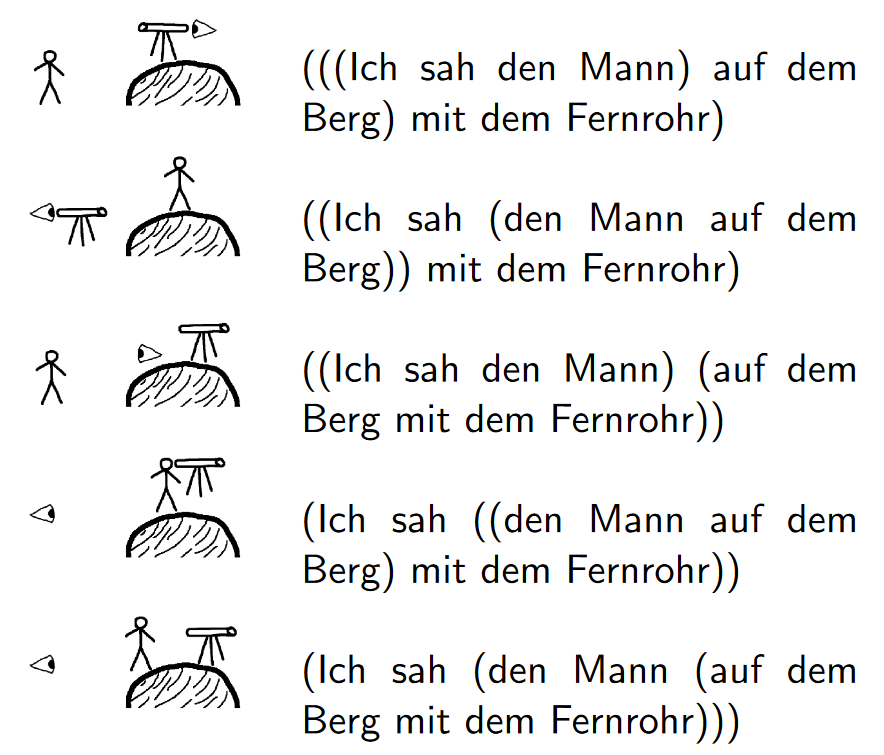
\includegraphics[width=0.7\textwidth]{img/fernrohr.png}  
    \caption[Nichteindeutigkeit nicht-formaler Modelle, KÖNIG Bettina: Vorlesung ''Modellierungsmethoden der Informatik'', \protect\url{ti.inf.uni-due.de/fileadmin/public/teaching/mod/slides/ws201112/einfuehrung.pdf}, 10.06.2019]{Nichteindeutigkeit nicht-formaler Modelle}\label{fig:fernrohr}
\end{figure} 
Ein \textbf{semiformales Modell} ist teilweise exakt. Es verfügt über eine definierte Syntax, spezifiziert aber nicht die ganze Domäne und verfügt über keine semantischen Konstruktionsregeln. Umsetzen lassen sich solche Modelle beispielsweise mit dem Entity-Relationship-Modell (ER-Diagramm), das anschließend ausführlicher beschrieben wird.
\\
\\
\textbf{Formale Modelle} verfügen über eine konkrete Syntax und Semantik. Das erlaubt die formale Definition von Modellen beispielsweise auf Basis deskriptiver Logiken.\footnote{Es gibt unterschiedliche Logiken, die sich in ihrer Ausdrucksmächtigkeit und Entscheidbarkeit unterscheiden.} Für formale Modelle lassen sich Algorithmen formulieren, die es erlauben Daten, die durch ein solches Modell beschrieben sind, automatisiert zu validieren. So beschriebene Modelle lassen sich in Datenmodelle überführen. Oder anders formuliert: formale Modelle können eindeutig mathematisch beschrieben werden.
\\
\\
Im Gegensatz zum Computer kann der Mensch auch mit informellen Modellen arbeiten. Man kann stark strukturierte und formalisierte Modelle, die algorithmisch genutzt werden können, offenen Modellen gegenüberstellen, in die sich ein Mensch hineindenken kann.
\\
Konzeptuelle oder auch konzeptionelle Modelle (\textbf{conceptual model}) bzw. Informationsmodelle (information model) sind beispielsweise in der Wirtschaftsinformatik von zentraler Bedeutung. Sie sind ein Werkzeug das die Kommunikation zwischen Informatik, Wirtschaftsinformatik und Wirtschaft erleichtert.\footcite[][S.44-47]{kobler2010qualitat} Genauso können solche Modelle in der interdisziplinären Arbeit zwischen Informatik, digitale Geisteswissenschaft und Geschichtswissenschaft fungieren.
\\
\\
Als \textbf{Datenmodelle} versteht man formale Modelle, die von Computern verarbeitbar sind und liegen aus diesem Grund in expliziter und eindeutiger Form vor. Datenmodelle dienen zur Repräsentation von konkreten oder abstrakten Objekte. JANNIDIS führt folgende Funktionen von Datenmodellen an:\footcite[][S.99-100]{jannidis2017grundlagen}
\begin{itemize}
\item Maschinelle Verarbeitung
\item Kommunikation in der Entwicklung von Algorithmen bzw. Software
\item Definition der Struktur der Daten für ein Programm
\item Standardisierung im Austausch von Daten
\end{itemize}
Zusammenfassend lässt sich sagen, dass der Modellbegriff, je nach Disziplin unterschiedlich verwendet wird. Gemeinsam jedoch ist stets die Funktion eine Domäne zu abstrahieren, zu vereinfachen und so zu beschreiben, dass dadurch Kommunikations- und Verstehensprozesse unterstützt werden. Zentral ist auch wie ein Modell beschrieben wird und welche Formen des Modellierens es gibt. Der aktive Prozess eine Domäne und ihre Daten in ein Modell zu überführen nennt man Modellieren.

\subsubsection{Modellierung}
\label{Modellierung}

\textcolor{red}{
Für McCARTY stellt die Modellerstellung, sprich das Modellieren, einen heuristischen Prozess dar, der die Manipulation und Konstruktion von Modellen umfasst. So, ganz im Sinne von STACHOWIAK, betrachtet er ein Modell als Repräsentation von etwas, dessen Zwecke der Entwurf zur Implementierung von etwas Neuen, oder der Analys einer Domäne dienlich ist.}\footcite[][S.255]{mccarty2004modeling}
\\
Drei Besonderheiten hebt JANNIDIS in der Modellierung von Daten in den Geisteswissenschaften hervor: die Historizität und Kontextabhängigkeit von Objekten, die für die geisteswissenschaftliche Analyse essentiell sind, die Unschärfe von Information und ''\textit{das systembedingte Primat des Individuellen vor dem Allgemeinen}''. Historizität meint, dass nicht nur jedes Objekt eine Geschichte aufweist, sondern auch jede Untersuchung eines Objektes. Als unscharf versteht man, dass es keine definitiven und fixen Werte gibt, die aber für eine maschinelle Verarbeitung notwendig sind. Und Letzteres meint, dass in den Geisteswissenschaften oft der Blick auf ein einzelnes Objekt, ein Roman, tendenziell interessanter ist als auf eine Vielzahl.\footcite[][S.106-108]{jannidis2017grundlagen}
\\
\\
In der Modellierung, auf einer konzeptuellen Ebene, ist es notwendig die im Bezug auf den Verwendungszweck wichtigsten Entitäten und ihre Attribute, sowie Relationen zu identifizieren.\footcite[][S.102-104]{jannidis2017grundlagen} Das \textbf{Entity-Relationship-Modell} (ER-Diagramm) ist eine Notationsformen, die genau auf diesen drei Begriffen beruht: Relationen, Attributen und Entitäten (Klassen). Die Entitäten -- alle potenziellen Untersuchungsobjekte -- verfügen über Eigenschaften, sogenannte Attribute. Weiters stehen sie zu anderen Entitäten in unterschiedlichen Beziehungen, sogenannten ''Relationen''.\footcite{chen1976entity} Eine gängige Art ER-Diagramme umzusetzen, besonders in der Softwareentwicklung, ist die \textit{Unified Modeling Language} (UML). Dabei handelt es sich um eine Sprache zur Modellierung, Dokumentation und Spezifikation von Systemen und Softwarekomponenten. Als ISO genormte Sprache definiert UML Bezeichner für wichtige Begriffe einer Modellierung und legt mögliche Beziehungen zwischen diesen Begriffen fest. UML definiert weiter grafische Notationen für diese Begriffe und für Modelle statischer Strukturen und dynamischer Abläufe, die man mit diesen Begriffen formulieren kann.\footcite{rumbaugh2004unified} Folgende Abbildung veranschaulicht die Bestandteile von UML:
\begin{figure}[H]
\centering
	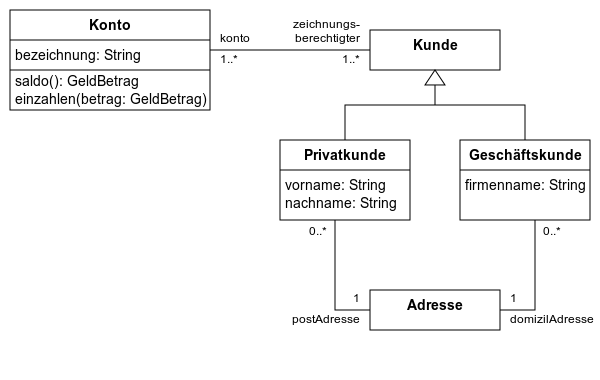
\includegraphics[width=0.9\textwidth]{img/uml.png}  
    \caption[Beispiel für ein Klassendiagramm nach UML, \protect\url{de.wikipedia.org/wiki/Unified_Modeling_Language}, 10.06.2019]{Beispiel für ein Klassendiagramm nach UML}\label{fig:uml}
\end{figure} 
Es existiert eine Klasse \textit{Kunden}, die wiederum zwei Unterklassen \textit{Privatkunde} und \textit{Geschäftskunde} besitzt. Die beiden Unterklassen (weißer Pfeil definiert 'hat Superklasse') unterscheiden sich in ihren unterschiedlichen Attributen. Wo die \textit{Privatkunde}-Klasse aus \textit{vorname} und \textit{nachname} vom Datentyp \textit{string} zusammengestellt wird, verfügt der \textit{Geschäftskunde} über das Attribut \textit{firmenname}. Die Linien zwischen den Klassen definieren Relationen und die daneben stehenden Zahlwerte und Symbole die Kardinalität dieser Beziehungen. So hat eine Instanz aus der Klasse \textit{Privatkunde} eine Relation \textit{postAdresse} zu einer Klasse \textit{Adresse}, aber eine Adresse kann mit mehreren Privatkunden verknüpft sein.\footcite[][S.99-108]{jannidis2017digital} 
\\
\\
Man kann nun aus der Klasse \textit{Privatkunde} beliebig viele Instanzen erzeugen. Instanzen entsprechen den eigentlichen Daten, die beispielsweise in einer Datenbank abgelegt werden können. So könne man das oben angeführte konzeptuelle Modell folgendermaßen instanziieren, sodass ein Privatkunde ''Christopher Pollin'' eine Adresse und ein Konto hat: 
\begin{itemize}
    \item[] Privatkunde --> \textit{vorname} ''Christopher'' \textit{nachname} ''Pollin''
    \item[] "Christopher Pollin" \textit{postAdresse} ''Neubaugasse 1''
    \item[] "Christopher Pollin" \textit{konto} ''Konto 1''
\end{itemize}{}

Die Beschreibung von historischen Daten und eines Modells, das diese Daten definiert, kann durch ER bzw. UML umgesetzt werden und hilft bei der Überführung in Datenmodelle. 
%%%%%%%%%%%%%%%%%%%%%%%%%%%%%%%%%%%%%%%%%%%%%
%%%%%%%%%%%%%%%%%%%%%%%%%%%%%%%%%%%%%%%%%%%%%
\subsubsection{Forschungsdaten in den Geschichtswissenschaften}
\label{forschungdaten}

Die Grundlage jeder formalen Verarbeitung sind Daten. Die Definition von Daten, im Sinne der Informationswissenschaft, lässt sich am besten in der Kontextualisierung mit drei anderen Begriffen fassen: Signal, Information und Wissen. Wo Signale eine physikalische Entität darstellen, beispielsweise eine Lichtwelle, versteht man unter Daten Zeichen zur Verarbeitung und Repräsentation von Information. Noch spezifischer wird der Begriff in der Informatik verwendet. In diesem Fach versteht man unter Daten Informationseinheiten, die für Maschinen lesbar und bearbeitbar sind. Von Information spricht man, wenn Daten in einem bestimmten Kontext interpretiert werden. WERSIG, aus einem kybernetischen Verständnis, spricht bei Information von einer ''\textit{Reduktion von Ungewissheit aufgrund von Kommunikationsprozessen}''\footcite[][S.74]{wersig1971information}. Noch eine Hierarchiestufe höher steht der Wissensbegriff. Wissen, so FAVRE-BULLE, ist gegeben, wenn ein kognitiver Agent, beispielsweise ein Mensch, auf Basis von Information eine Handlung in der Welt setzt.\footcite[][S.93-97]{favre2001information} Folgende Darstellung zeigt die Abhängigkeit dieser 4 Begriffe zueinander, mit einem anwachsen der Komplexität der Struktur, sowie der Anbindung an einen kognitiven Agenten.\footcite[Eine ausführlichere Auseinandersetzung mit den Begriffen Daten, Information und Wissen findet sich in meiner ersten Abschlussarbeit.][Masterarbeit Graz, S.20-28]{pollin2017suchen}
\begin{figure}[H]
\centering
	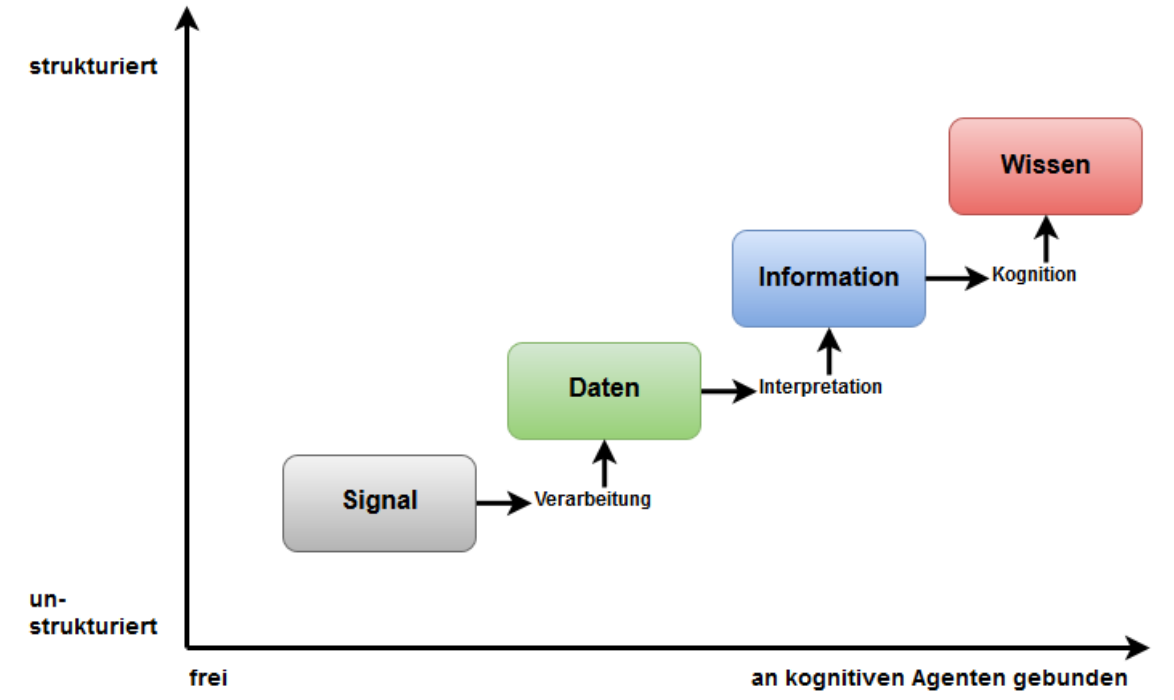
\includegraphics[width=0.85\textwidth]{img/daten.png}  
    \caption[Signal, Daten, Information und Wissen. POLLIN Christopher: Vom Suchen, Stöbern und Finden : Information Retrieval am Beispiel der Digitalen Sammlung des Hans Gross Kriminalmuseums, Masterarbeit Graz, S.21 ]{Signal, Daten, Information und Wissen} \label{fig:daten}
\end{figure} 
Entstehen Daten während eines, oder als Ergebnis eines Forschungsprozesses, so spricht man von \textbf{Forschungsdaten}. Damit werden sowohl Daten aus den Naturwissenschaften (Messdaten aus einem Experiment), Sozialwissenschaften (Interviews) oder den Kulturwissenschaften (dokumentierte Beobachtung) zusammengefasst.\footcite[][09.06.2019]{kindling2013forschungsdatenmanagement}
\\
ANDORFER spricht sich für einen nicht ''\textit{inflationären Gebrauchs dieses Begriffes}'' und einer ''\textit{präzisere[n] Terminologie}'' im Zusammenhang des Begriffes geisteswissenschaftliche Forschungsdaten aus. Es soll klar definiert sein, was man als Forschungsdaten auffasst und was davon ausgeschlossen ist. Weiters soll es bei den für Fachwissenschafter*innen vertrauten Begrifflichkeiten bleiben.\footcite[][]{andorfer2015forschungsdaten}
Diese Datenpyramide, in Abbildung \ref{fig:forschungsdaten}, beschreibt, dass aus den Kulturerbeeinrichtungen (Archiv, Bibliothek und Museum), sowie den digitalen Repositorien, die Quellen für die Fachwissenschaftler*innen zur Verfügung gestellt werden. Beispielweise liegen die originalen und analogen historischen Rechnugnsbücher in einem Stadtarchiv. Wird auf Basis dieser Quellen, und man sieht bereits, dass die Pyramide schmäler wird und eine Selektion alle vorhanden Objekte geschieht, eine weitere Leistung produziert, wie etwa eine Transkription des Rechnungsbuch. In diesem Fall kann man von Arbeitsdaten sprechen. Solche Arbeitsdaten sind Forschungsdaten und können in einem geeigneten Repositorium gesichert und verfügbar gemacht werden. Ein solches Repositorium ist beispielsweise GAMS.\footnote{Geisteswissenschaftliches Asset Management System, \url{https://gams.uni-graz.at}, 06.05.2020.} Eine weitere Auswahl führt von Arbeitsdaten zu veröffentlichten Publikationen, also ein Aufsatz oder eine digitale Edition, dessen Grundlage die Transkription eines Rechnungsbuch war.
\begin{figure}[H]
\centering
	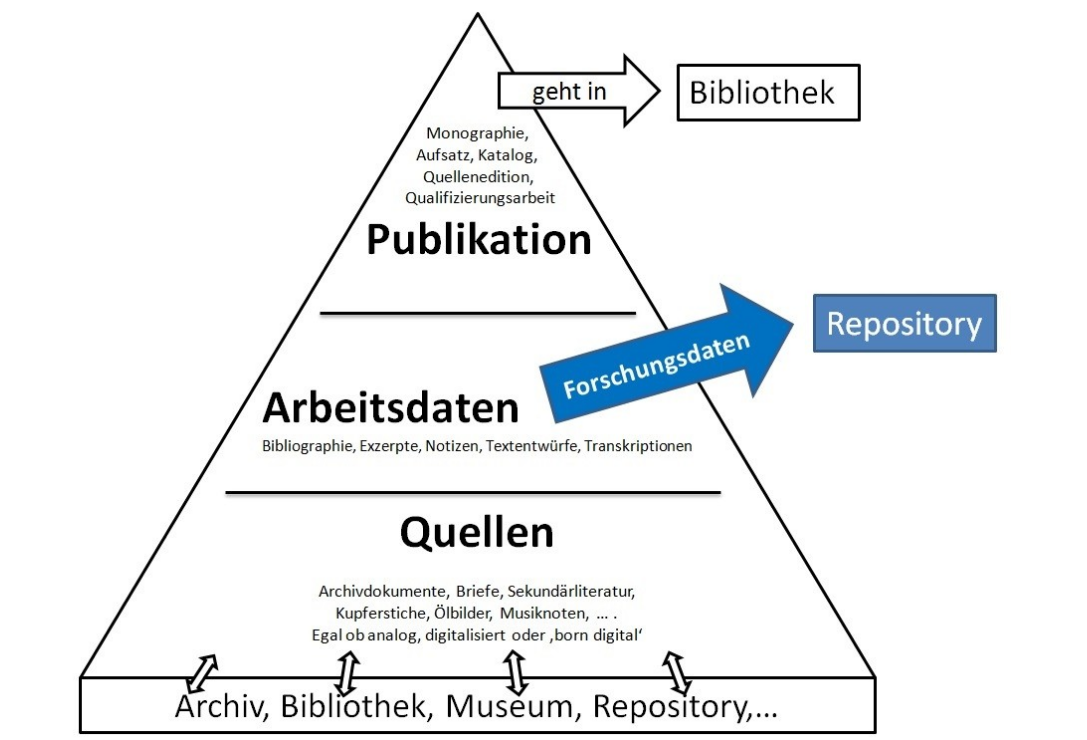
\includegraphics[width=0.85\textwidth]{img/forschungsdaten.png}  
    \caption[Datenpyramide geisteswissenschaftlicher Forschungsdaten im institutionellen Kontext, ANDORFER, Peter: Forschungsdaten in den (digitalen) Geisteswissenschaften: Versuch einer Konkretisierung, 2015, S.14]{Datenpyramide geisteswissenschaftlicher Forschungsdaten im institutionellen Kontext nach ANDORFER} \label{fig:forschungsdaten}
\end{figure} 
Für die Geisteswissenschaften und im speziellen für die Geschichtswissenschaften, in denen viel stärker hermeneutischer Prozess im Vordergrund stehen, ist der Begriff der Forschungsdaten nicht eindeutig. HILTMANN sieht einen engeren und einen weiteren Begriff von Forschungsdaten in den Geschichtswissenschaften. Im engeren Sinne versteht man Metadaten als Annotationen von historischen Quellen in all ihren Ausprägungen. Als Beispiel ist die archivalische Erschließung eines Quellenkorpus angeführt, damit die Verwahrung und Auffindbarkeit für eine potentielle, wissenschaftliche Auseinandersetzungen ermöglicht wird. Im weiteren Verständnis kann alles, das digital vorhanden ist, zur historischen Quelle und somit zu relevanten Daten für die Geschichtswissenschaft werden.\footcite[][09.06.2019.]{hiltman2018forschungsdaten}
\\
\\
Damit Forschungsdaten nachnutzbar und nachvollziehbar sind bedarf es eines mitgelieferten Modells. Diese Modelle wiederum müssen auf Standards beruhen. Es ist zeitintensiv die Datenmodelle andere Fachwissenschaftler*innen zu verstehen und oft ist es leichter sein eigenes Modell zu entwickeln. Ein generelles Problem mit Informationssystem und Forschungsdaten ist, dass sie nur für eine bestimmte Fragestellung bzw. ein bestimmtes Projekt entwickelt wurden. Werden bei der Generation der Forschungsdaten aber bereits Konzepte und Standardisierungen verfolgt, so fällt es leichter die ''Datensilos'' zu verlassen und die Nachnutzung zu fördern. 
\\
Eine erste Form der Standardisierung in den (digitalen) Geisteswissenschaften ist die \textit{Text Encoding Initiative} (TEI). Wenn auch die Umsetzungen der TEI nicht einem 'klassischen' Standard entspricht, so sind die Überlegungen, wie man Text strukturieren und annotieren kann, sehr wohl standardisiert. 
\\
Es ist eine Notwendigkeit, dass Standards auf der einen Seite ausdrucksstark sein müssen, um die unterschiedlichen Problemstellungen fassen zu können, andererseits es sich aber daraus formale Modelle ableiten lassen müssen. THALLER fordert deswegen, dass die Standards zur Beschreibung von Modellen eher beschreibend statt vorschreibend sein sollen.\footcite[][S.204]{thaller2017need}


%%%%%%%%%%%%%%%%%%%%%%%%%%%%%%%%%%%%%%%%%%%%%
\newpage
\section{Historische Rechnungsbücher als Quelle}
\label{ref:Rechnung}

In diesem Kapitel wird der Quellentypus Rechnungsbuch als historische Quelle dargestellt. Dazu werden inhaltliche, wie auch äußerliche Eigenschaften von Repräsentanten dieser Quellengattung beschrieben und die dazugehörige Fachliteratur diskutiert.
Anfangs wird der Quellentypus an sich beschrieben, gefolgt von einer Beschreibung konkreter digitale Editionsprojekte von Rechnungsbüchern, in denen ein Blick auf die textuelle und semantische Strukturen der Quellen geworfen wird. Weiters wird erörtert, welche geschichtswissenschaftlichen Forschungsfragen sich damit beantworten lassen.

%%%%%%%%%%%%%%%%%%%%%%%%%%%%%%%%%%%%%%%%%%%%%
\subsection{Wirtschafts- und Rechnungsbücher}

''\textit{Wirtschafts- und Rechnungsbücher kennen keinen Grenzen -- keine räumlichen, wenig ständische, keine institutionellen Grenzen -- und auch keine disziplinären.}''\footcite[][S.51]{gleba2016rechnen}
\\
\\
Bei Rechnungsbüchern handelt es sich um pragmatisches, oft serielles, zum Teil über Jahrzehnte hinweg erhaltenes, aus dem Alltag der Menschen stammendes Schriftgut, das zur Dokumentation und als Gedächtnisstütze für den Austausch von Waren, Dienstleistungen und Rechten diente. Zu meist auf Papier, aber im Laufe der Zeit mittels unterschiedlichsten Schreib-- und Beschreibstoffen und ohne übergeordnete Standards verfasst, folgen sie keinem repräsentativen Zweck. Menschen mussten zumindest über Schreib- und Lesekenntnisse verfügen, die von einfachen Rechenfertigkeiten bis hin zur Erstellung vollständiger Kalkulationen reichen. Das gemeinsame Element dieses differenzierten Quellentypus ist die Ausrichtung auf wirtschaftliche Aktivitäten in Form von Transaktionen. Daraus ergibt sich eine ''natürliche'' -- oft auch textuelle -- semantische Struktur, die zeigt, das es sich um ein ''\textit{Werkzeug des Alltages}'' gehandelt hat, das man an unterschiedlichen Orten und Zeiten der Menschheitsgeschichte finden kann.
\\
\\
Eine Transkription allein reicht nicht aus, um die linguistische/textuelle, quantifizierbare und die semantische Dimension einer solchen Quelle abzudecken. Vielmehr ist es die Edition der Quellen, die dabei helfen kann, Forschungsinteresse zu befrieden. So wird die Vielfalt der ableitbaren Inhalte aus Rechnungsbüchern, sowie die Möglichkeiten der ''\textit{interdisziplinären Erschießung der Quelle Rechnungsbuch}'' hervorgehoben. Die Herausforderungen der Erschließung der Quelle sind vielfältig: Maß-, Größen- und Gewichtsordnungen und Information zu Geldwerten sind abhängig von Ort und Zeit. Dennoch lassen sich viele Forschungsfragen aus unterschiedlichen Disziplinen neben den Geschichtswissenschaften, wie etwa der Historischen Linguistik, der Editions- oder Medienwissenschaft, mit solchen Quellen bearbeiten: wie haben sich Güter, Dienstleistungen und Geldgeschäfte über die Zeit hinweg verändert, welche wirtschaftlichen, aber besonders auch welche kultur-- und sozialgeschichtliche Relationen gibt es? Rechnungsbücher gehen nach KLAPP ''\textit{weit über wirtschafts-- und verwaltungsgeschichtliche
Aspekte hinausgehen}''\footcite[][S.14]{klapp2011rechnung} und so erlauben Fragestellungen dieser Art weitere soziale, gesellschaftliche und wirtschaftliche Implikationen, die uns ein Verständnis darüber geben können, wie das Leben der Menschen in der Vergangenheit ausgesehen haben kann.\footcite[][S.7-10]{gleba2015einleitung}
\\
\\
GLEBA unterscheidet vier Kategorien\footcite[][S.51-54]{gleba2016rechnen} in diesem Zusammenhang:
\begin{itemize}
\item \textbf{Urbare} sind Besitzverzeichnisse, in denen Besitzrechte einer Grundherrschaft und der damit verbundenen Abgaben aufgelistet werden. Hier finden sich meist auch Angaben zur Lokalisierung der Liegenschaften.
\item Sogenannte \textbf{Heberegister} beinhalten die Abgabepflichten an wirtschaftlichen Gütern, wie Arbeit oder Naturalien.
\item In \textbf{Wechselbüchern} wird der Wechsel von Menschen in einer anderen Grundherrschaft dokumentiert. 
\item \textbf{Rechnungsbücher} führen vor allem Transaktionen, sprich monetäre Einnahmen und Ausgaben an. Sind aber nicht nur auf diese beschränkt.
\end{itemize}
BRUCH sieht Rechnungsbücher als geeignete Quelle, aus denen Daten zur Beantwortung der oben angeführten Forschungsfragen extrahiert werden können. Diese können anschließend mittels quantitativen Methoden weiterverarbeitet werden. Am Quellenbestand des \textit{Zisterzienserinnenkloster Pielenhofen bei Regensburg}, der beispielhaft für die Arbeit in diesem Bereich steht, wird diese Vorgehensweise veranschaulicht. Nach einer notwendigen Kontextualisierung der Quelle, datiert auf 1224-1348, wird die wirtschaftliche Situation des Klosters über diesen Zeitbereich hinweg, beschrieben. BRUCH kommt zu folgendem Schluss:\footcite[][S.13-37]{bruch2015daten}
\\
\\
''\textit{Allerdings zeigt sich auch, dass die für ein Jahr gewonnenen Daten miteinander in Beziehung gesetzt werden können: Einnahmen gegenüber Ausgaben, Getreide gegenüber Geld, Schulden gegenüber Einnahmen und Ausgaben, Klosterinsassen oder der Viehbestand gegenüber den Einnahmen bzw. Ausgaben. [...] So wandeln sich die reinen Daten in Informationen, die zur Beantwortung konkreter Fragestellungen herangezogen werden können.}''\footcite[][S.37]{bruch2015daten}
\\
\\
BRUCH kommt zum Schluss, dass die Abrechnung durch das Mutterkloster nicht auf einem Rechnungsjahr basiert und so die Bezugszeiträume für die Zahlen nicht zur Gänze nachvollziehbar sind. Die lückenhafte Überlieferung ist eine Momentaufnahme und somit eine mathematisch-statistische bzw. quantitative Analyse nur in Ansätzen möglich. Nichtsdestotrotz lassen sich die Daten aus dem Rechnungsbuch in Informationen überführen. Folgendes lässt sich Gegenüberstellen und auf dieser Informationsbasis weiter untersuchen:\footcite[][S.37-44]{bruch2015daten}
\begin{itemize}
\item Die Haushaltsführung, sprich Einnahmen und Ausgaben eines Jahres 
\item Getreide- und Geldeinnahmen bzw. Ausgaben, um die wirtschaftlichen Schwerpunkte des Klosters zu eruieren.
\item Schulden können gegen die Einnahmen aufgerechnet werden 
\item Die Zahl der Klosterinsassen oder der Viehbestand können mit Einnahmen bzw. Ausgaben in Verbindung gebracht werden. Hinzu kommt, dass man, wenn man die unterschiedlichen Visitationszeitpunkte beachtet,
Tendenzen ausmachen kann, ob die Klöster mit strukturellen Defiziten zu recht kommen musste, oder prosperierten.
\end{itemize} 

%%%%%%%%%%%%%%%%%%%%%%%%%%%%%%%%%%%%%%%%%%%%%
%%%%%%%%%%%%%%%%%%%%%%%%%%%%%%%%%%%%%%%%%%%%%
\newpage
\subsection{Digital Edition Publishing Cooperative for Historical Accounts}
\label{DEPCHA}

''\textit{Thus, the information that is available about the past is grounded in verifiable facts based on evidence that we make available to everyone. We’re demonstrating the importance of evidence and facts in understanding our world.}''\footnote{TOMASEK Kathryn: Accounting for the past,\url{https://wheatoncollege.edu/news/accounting-for-the-past}, 30.01.2020.}
\\
\\
Daten - aus unterschiedlichen Formaten - sollen auf einer gemeinsamen Plattform zusammengeführt werden und adäquate Formen des Retrievals, der Discovery und der Visualisierung eröffnen, um die Arbeit mit den Quellen zu erleichtern. Die Überführung in das Resource Description Framework (RDF) auf Basis der im Projektkontext entwickelten \textit{Bookkeeping-Ontologie}, die Transferprozesse historischer Rechnungsbücher formalisiert, erlaubt die Interoperabilität, Verlinkung und das Zusammenführen von Informationen im Sinne des \textit{Web of Data} und \textit{Linked Open Data}. Diese Begriffe werden im Kapitel \ref{WebofData} ausführlich behandelt.
\\
\\
\textcolor{red}{
Drei ausgewählte Rechnungsbücher, die im Zuge von DEPCHA bearbeitet und veröffentlicht werden, werden nun ausführlicher behandelt. Dabei wird sowohl die Struktur und der Kontext der Quelle beschrieben und herausgearbeitet welche Forschungsinteressen mit diesen Quellen bedient werden können. 
}

\subsubsection{The George Washington Financial Papers}

Die digitale Edition der \textit{George Washington Financial Papers} (1748-1799) haben zum Ziel die Geschäfts- und Haushaltsakten des US-Präsidenten George Washington über das Web zugänglich zu machen. Basierend auf einer technischen Open Source Lösung, dem Content Management System Drupal\footnote{Drupal, \protect\url{drupal.org}, 12.10.2019}, sind Benutzer*innen in der Lage die Transkriptionen der drei Rechnungsbücher (\textit{Ledgers A, B, and C}) von Washington zu lesen, Suchanfragen an die aus den Editionen extrahierten Daten zu stellen, sowie die Daten zu exportieren und lokal weiter zu verarbeiten. Auf diese Weise wird ein Einblick in das Leben der Person George Washington, sowie  anderer Themen, wie etwa die materielle Kultur, Sozialgeschichte, Gewerbe und Landwirtschaft dieser Zeit ermöglicht.\footnote{The George Washington Financial Papers Project, \protect\url{financial.gwpapers.org}, 08.10.2019.} Beispielhafte Forschungsfragen, die für Historiker*innen im Zuge dieses Editionsprojektes von Interesse sind, lauten wie folgt: 
\begin{itemize}
\item Wie viel Geld hat Washington jährlich für bestimmte Rohstoffe ausgegeben?
\item Welche Rolle spielt der Sklavenhandel in Washingtons wirtschaftlicher Tätigkeit?
\item Wie hat sich der Preis bestimmter Rohstoffe über diesen Zeitraum hinweg verändert?
\item Wie sieht das Netzwerk der Geschäftspartner rund um Washington aus?
\item Wie wurde der Wert der Ware Tabak in verschiedenen Währungen berechnet und bewertet?
\end{itemize}
Im Laufe seines Lebens trug Washington Tausende von Finanzdokumenten zusammen, in denen er jede Transaktion genau nach modernster Finanzlehre aufzeichnete. Dies umfasste Ausgaben für Lebensmittel und Textilien oder seinen Landsitz in Mount Vernon, sowie Kosten für die Ausbildung seiner Kinder oder die medizinischen Behandlungen für Sklaven. Weiters dokumentiert Washington an wen er Geld verliehen hat, seine Anteile an Firmen oder eingehobene Mieten.
Aus den Rechnungsbüchern schließt STERTZER, dass Washington ein versierter Unternehmer war, der Innovationen suchte, kalkulierte Risiken einging und aufgrund seiner methodischen Buchführung ein breites Verständnis für die amerikanische Wirtschaft hatte.\footcite[][]{stertzer2014working}
\\
\\
Abbildung \ref{fig:washington} zeigt die erste Seite aus dem Rechnungsbuch \textit{Ledger A} von Washington. Aus der Transkription der ersten 3 Einträge erkennt man eine Struktur, wie sie typisch ist für ein US amerikanisches Rechnungsbuch dieser Zeit ist. Die Überschrift definiert die Debit-Seite der Transaktionen, gekennzeichnet durch die Abkürzung \textit{Dr}, mit der Person \textit{George Fairfax} der nun folgenden Einträge. In der ersten Spalte wird das Datum der Transaktion festgehalten, wie ''\textit{Novr 6}'' für den 06.11.1750, gefolgt von der Verschriftlichung der Transaktion in der mittleren Spalte. Diese definiert zu meist den Status, Art, Wert und die beteiligten Personen der Transaktion. ''\textit{To Ditto}'' meint, dass es sich um die zuvor angeführte Person handelt. Für eine formale Verarbeitung müssen diese Phrasen normalisiert werden. Die letzten 3 Spalten stehen für die Währungseinheiten Pfund, Schilling und Pence. Zum Teil werden diese Spalten auch genutzt um eine (Zwischen)Summe zu berechnen.\footnote{Ledger A, 1750 - 1772: pg.1, \protect\url{financial.gwpapers.org/?q=content/ledger-1750-1772-pg1}}
\\
\\
\begin{tabular}{clcc}
& \textbf{George Fairfax Esqr. Dr}\\
1750 April 2 & To John Welton's Order on you & 4 & 10\\
Octr 7 & To Cash lent & 2 & 3 \\
Novr 8 & To Ditto paid Robt Worthington \& Michl Sweim Chr Govr &  17 & 3\\
\end{tabular}
\medskip
\begin{center}
\textit{Transkription von drei Einträge von Seite 1 des Ledger Book A}
\end{center}
Inhaltlich zusammengefasst lassen sich 3 Geldzahlungen von George Washington an \textit{George Fairfax} festmachen. Einmal eine Zahlung in Zusammenhang einer weiteren Person \textit{John Welton's Order}, ein anderer Geldbetrag von 2 Pfund und 3 Schilling der verliehen wurde und die Bezahlung für \textit{Robt Worthington \& Michl Sweim}.

\begin{figure}[H]
\centering
	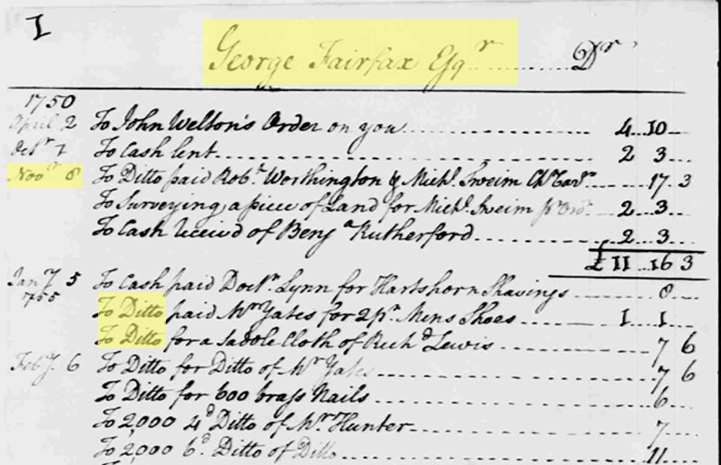
\includegraphics[width=1\textwidth]{img/washington.png}  
    \caption[1. Seite von George Washington, 1750-72, \textit{Ledger Book A}, Library of Congress, Manuscript Division, STERTZER Jennifer: \protect\url{doi.org/10.16995/dscn.57}]{1. Seite von George Washington, 1750-72, \textit{Ledger Book A}, Library of Congress, Manuscript Division.} \label{fig:washington}
\end{figure}


\subsubsection{Cameron Family Papers, Stagville Accounts}

Das historische Stagville ist eine Tabakplantage nördlich von Durham (North Carolina, USA), die seit dem späten 18. Jahrhundert im Besitz der Familie Bennehan und Cameron ist. Ihr Eigentum, vor Beginn des Amerikanischen Bürgerkriegs, umfasste 30.000 Hektar Land und um die 900 versklavten Menschen, die auf dieser Plantage arbeiten mussten.\footcite[][]{brumfield2015medea}
\\
Die \textit{Cameron Family Papers} (1767-1892) beinhalten umfangreiche Geschäftsunterlagen im Zusammenhang mit einem Wirtschaftsbetrieb rund um eine Tabakplantage, die Transaktionen zwischen dem Geschäftsladen und den Mitgliedern, sowie unfreien Arbeiter*innen der Gemeinschaft dokumentieren. Beispielsweise findet sich darin ein sogenanntes ''\textit{Slave-Ledger}''. Dabei handelt es sich um ein separat geführtes Rechnungsbuch, das Transaktionen zwischen dem Geschäft auf der Tabakplantage und versklavten Kunden*innen dokumentiert.
\\
AGBE-DAVIS und BRUMFIELD stellen bei der Untersuchung des ''\textit{Slave-Ledger}'' fest, dass die Unterlagen nicht isoliert, sondern nur im Kontext aller Dokumente in den \textit{Cameron Family Papers} betrachtet werden müssen. Forschungsfragen in diesem Projektkontext sind:
\begin{itemize}
\item Wie bezahlen unfreie Arbeiter*innen Güter, die sie im Laden der Plantage erwerben konnten?
\item Welche wirtschaftlichen Abhängigkeiten (Verschuldungen) bestehen zwischen den unterschiedlichen Akteuren?
\item Welche Waren werden gemeinsam gekauft?
\item Welche soziale Stellung haben sie und inwieweit beeinflusst das ihre Einkäufe.
\end{itemize}
In folgender Abbildung ist die dritte Seite des Rechnungsbuches aus Stagville dargestellt.\footnote{Stagville Accounts, From the Page, \protect\url{fromthepage.com/agbedavies/stagville-accounts/00133-sv0061/display/7884}, 08.10.2019.} Der erste Eintrag beschreibt den Kauf eines Schuhmessers zum Preis von 1 Schilling und 6 Pence. Im ''\textit{Slave-Ledger}'' verkauft Cameron, aber ein Schuhmesser für 2 Schilling. Ob die Änderung des Preises durch den zeitlichen Unterschied gegeben ist, oder eben durch den sozialen Status der kaufenden Person, ist eine relevante geschichtswissenschaftliche Fragestellung.\footcite[][]{brumfield2019blog}
\begin{figure}[H]
  \centering
  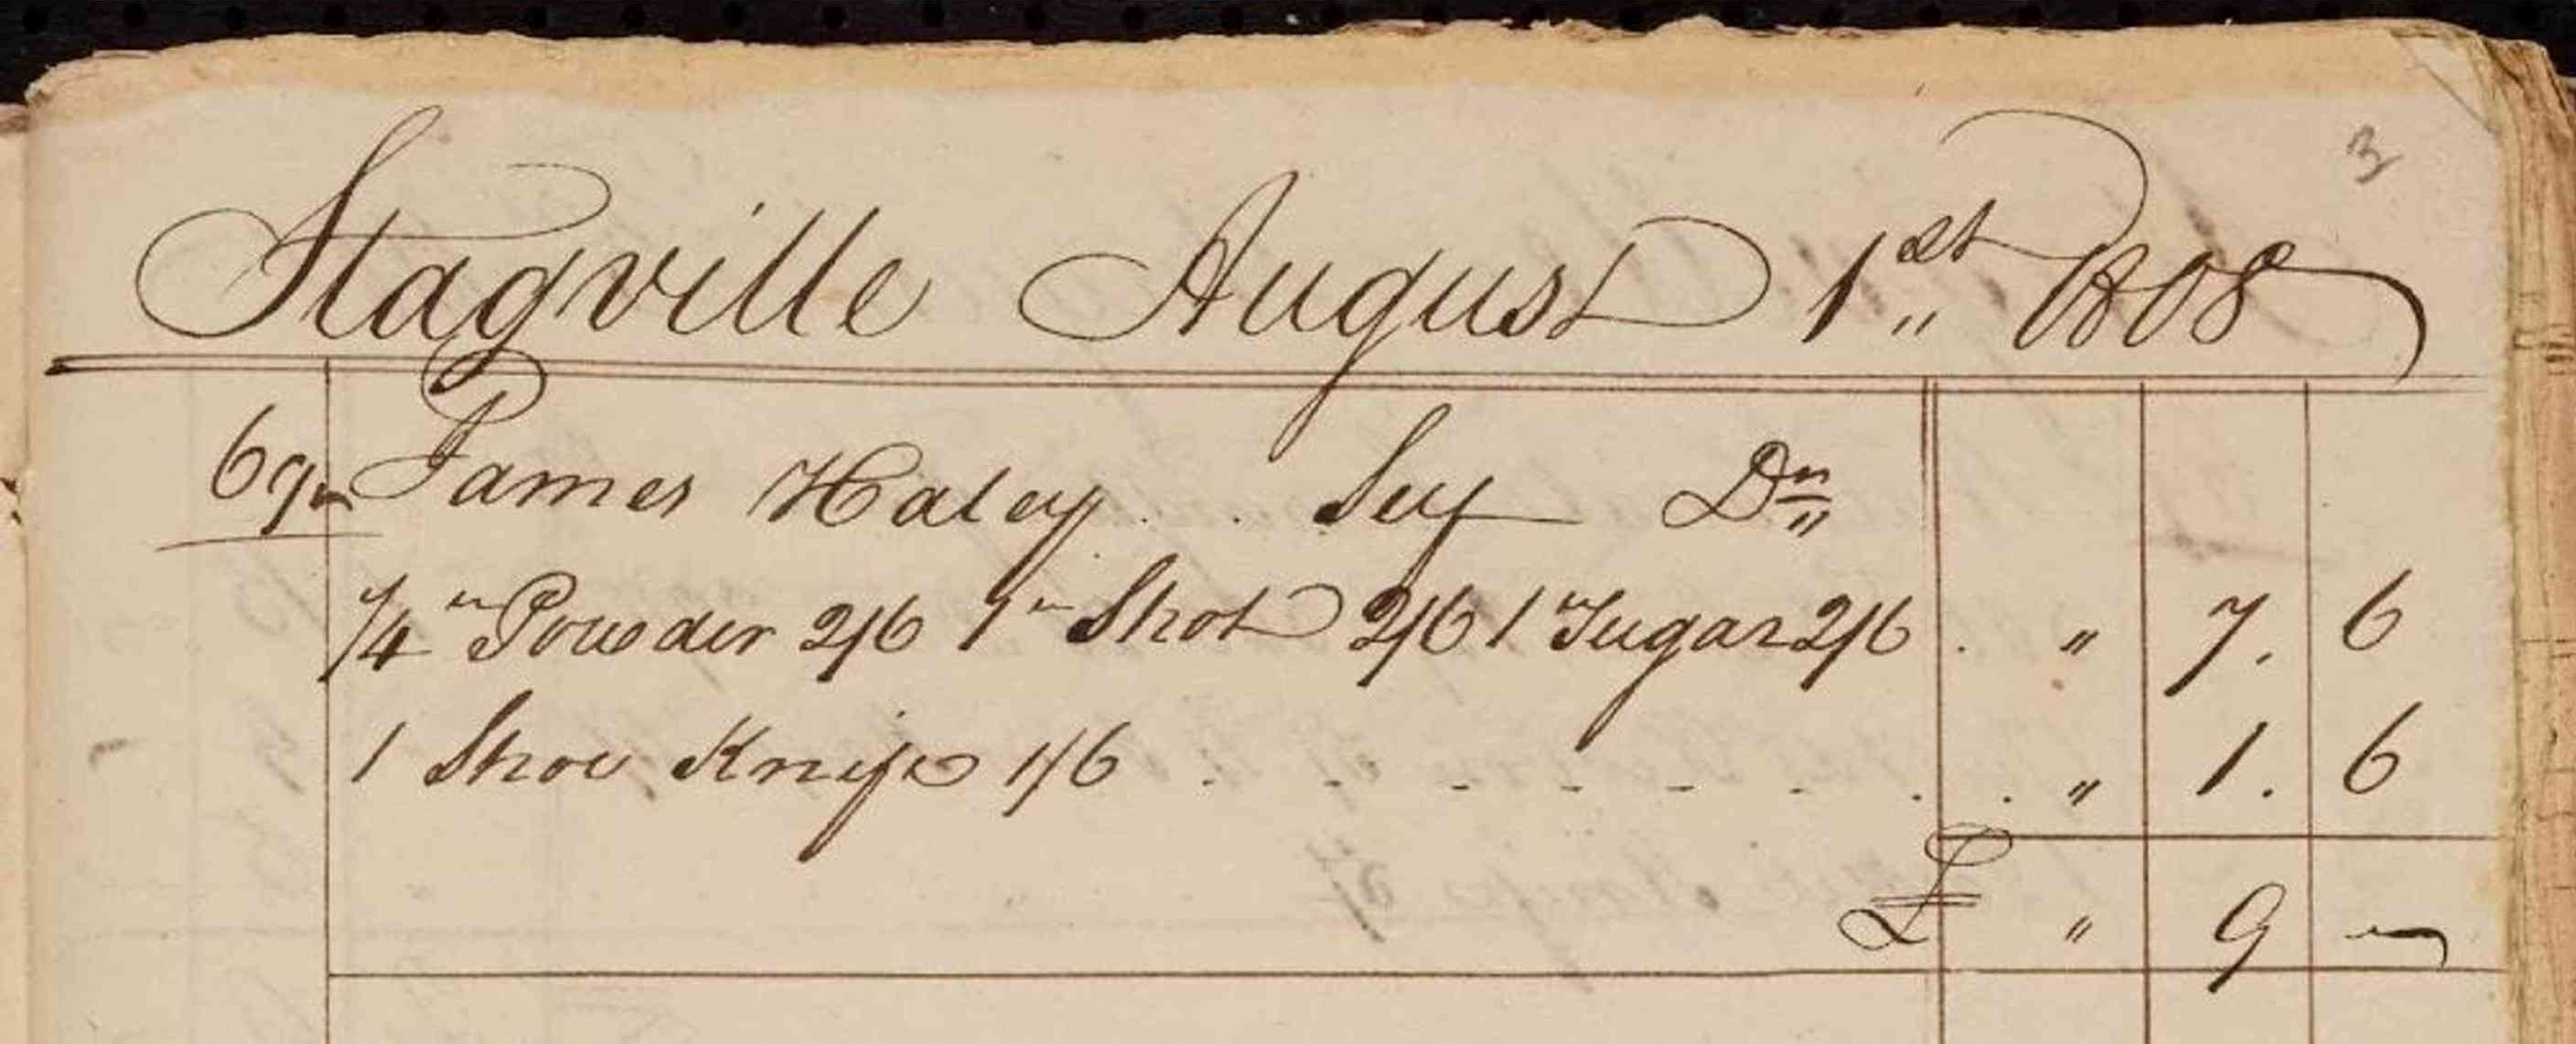
\includegraphics[width=1\textwidth]{img/stagville.jpg}  
  \caption[Seite 3 des Objektes \textit{00133\_sv0061} der Stagville Accounts, \protect\url{fromthepage.com/agbedavies/stagville-accounts/00133-sv0061/display/7884}]{Seite 3 Objektes \textit{00133\_sv0061} der Stagville Accounts} \label{fig:stagville}
\end{figure}
\begin{tabular}{clcc}
  & \textbf{Stagville August 1st 1808}\\
 69 & James Haley Self Dr. & &\\
    & 1/4 lb Powder 2/6 1 lb Shot 2/6 1 lb Sugar 2/6 & 7 & 6\\
	& 1 Shoe Knife 1/6  & 1 & 6\\
	& & 9  & -
\end{tabular}
\medskip
\begin{center}
\textit{Transkription der zweier Einträge auf Seite 3 der Stagville Accounts.}
\end{center}
In Abbildung \ref{fig:stagville} findet sich wieder eine ganz ähnliche Struktur. In der Überschrift wird Ort und Datum, der 1. August 1808, angegeben und alle nun folgenden Einträge beziehen sich darauf. Die tabellarische Struktur verfügt über 5 Spalten. Die erste Spalte enthält eine Referenz auf eine Seite in einem anderen Dokument, in denen die \textit{Credit} gegen geschrieben werden. Die zweite Spalte beinhaltet den Fließtext der Einträge, wobei die Nennung der Person in der ersten Zeile jede weitere Zeile als einen eigenen Eintrag mit Geldbeträgen in der 4. und 5 Zeile deklariert. Inhaltlich zusammen gefasst hat ''James Haley'' einen 1/4 Pfund Pulver, einen Pfund Munition und einen Pfund Zucker zum Preis von je 2 Schilling und 6 Pence, sowie ein Schumesser zum Preis von 1 Schilling und 6 Pence käuflich erworben. Die Summer alle Einträge ist somit 9 Schilling, da 1 Schilling 12 Pence entspricht.

\subsubsection{The Wheaton Accounts}

Die \textit{Wheaton Family Papers} umfassen mehrere Bücher im Zeitraum von 1828 bis 1859, die unter anderem die finanziellen Geschäfte von \textit{Laban Morey Wheaton}, einem Geschäftsbesitzer eines \textit{dry goods store} aus Norton, Massachusetts in den Vereinigten Staaten von Amerika, dokumentieren. Unter \textit{dry goods} versteht man einen aus dem 17. Jahrhundert stammenden historischen Begriff, der je nach Region zum Teil unterschiedliche Güter zusammenfasst. Darunter werden im Allgemeinen Produkte verstanden, die ''trocken'' sind, beispielsweise Textilien, Konfektionskleidung, Tabak oder bestimmte Lebensmittel, wie etwa Kartoffel.\footcite[Definition von \textit{Dry Goods}, \protect\url{chestofbooks.com/reference/Dictionary-of-Dry-Goods/Dry-Goods.html}, 23.05.2019,][]{cole2015complete}
\\
Die Stadt Norton ist eine charakteristische Kleinstadt im Nordosten der USA, die landwirtschaftlich und von Manufakturen geprägt ist. Sie befindet sich im Hinterland der regional bedeutenden Häfen Boston, New Bedford, Newport und Providence. In einer Geschichte der Stadt Norton von CLARK wird \textit{Laban Morey Wheaton} namentlich genannt. Er lebte von 1796 bis 1865, hat Rechtswissenschaften an der \textit{Brown University} studiert und jahrelang als \textit{Postmaster of Norton} gearbeitet. Er war politisch aktiv und war Vertreter im \textit{Massachusetts General Court}, sowie Mitglied im \textit{Massachusetts Governor's Council}. Weiters war er verheiratet und Angehöriger des Kongregationalismus, einer Form der christlichen Gemeindeverfassung. Die Wheaton Familie besaß eine Milchviehherde und Manufakturen zur Produktion von Baumwollwatte, die \textit{Wheaton Manufacturing Company,} und eine zur Produktion von Strohhüten\footcite[][S.6]{tomasek2013encoding}. So gehört Laban Wheaton zu einem der wohlhabensten Männer der Stadt. Sogar ein Portrait von ihm ist bei CLARK überliefert.\footcite[][S.496]{clark1859history} 
\begin{figure}[H]
\centering
	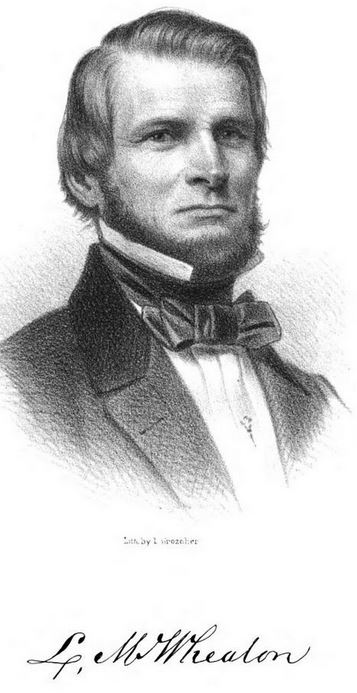
\includegraphics[width=0.2\textwidth]{img/LMwheaton.jpg}  
    \caption[Portrait von Laban Morey Wheaton, CLARK, George Faber: A History of the Town of Norton, Bristol County, Massachusetts, from 1669-1859.
Crosby, Nichols, and Company, and author at Norton, 1859, S.497.]{Portrait von Laban Morey Wheaton} \label{fig:LMwheaton}
\end{figure} 
Aus dieser Überlieferung über \textit{Laban Morey Wheaton} kann man die These aufstellen, dass er ein mächtiger Mann war. Auf der einen Seite politisch aktiv und politischer Vertreter, auf der anderen Seite vermögend und Besitzer mehrere Immobilien und eines Geschäftes. Gerade der im \textit{daybook} dokumentierte Verkauf von Gütern, in dem Menschen Lebensmittel im Austausch für Arbeit erwerben, zeigt eine gewisse Machtposition. Denn die, nicht vollständig überlieferten Rechnungsbücher von Wheaton, zeigen neben Angaben zu Gütern, Dienstleistungen und Geldbeträgen in den einzelnen Transaktionen, auch eine Vielzahl von Individuen und ihrer Familien, die in Beschäftigung oder anderen Verhältnissen zu Wheaton stehen, oder an die er Objekte, Tiere und Gebäude vermietete. TOMASEK führt an, dass diese Rechnungsbücher detaillierte Informationen über das tägliche Leben der Einwohner*innen in New England geben. Ein städtisches Leben, das durch eine gemischte Land-, sowie Industriewirtschaft im zweiten Quartal des 19. Jahrhunderts, geprägt ist.\footcite[][S.5]{tomasekmedea}
\\
\\
Das \textit{Wheaton College Massachusetts} stellt die \textit{Wheaton Family Papers} Dokumente in ihrem digitalen Repositorium online zur Verfügung.\footnote{Wheaton Family Papers, \url{digitalrepository.wheatoncollege.edu/handle/11040/7928}, 19.05.2019.} Die wissenschaftliche Auseinandersetzung erfolgt durch Kathryn Tomasek, Professorin für Geschichte am \textit{Wheaton College Massachusetts}. Im Zuge des Projektes \textit{The Wheaton College Digital History Project} wurden Teile der Wheaton Paper, darunter beispielsweise das oben angeführte \textit{daybook} gemeinsam mit Studierenden transkribiert und mit dem Standard der Text Encoding Iniative (TEI) ausgezeichnet und im Sinne einer Vorarbeit einer digitalen Edition ediert. Der Fokus dieser Arbeiten liegt auf der Erschließung der einzelnen Transaktionen und der damit verbundenen Personen, Güter und Dienstleistungen.\footcite[TOMASEK Kathryn: The Wheaton College Digital History Project: Undergraduate Research in a Local Collection, \protect\url{writinghistory.trincoll.edu/teach/wheaton-college-digital-history-project-tomasek}, 23.05.2019.][S.379]{alexander2012should} Teile davon wurden im Zuge des DEPCHA Projektes für die Umsetzung eines Prototyps zur Publikation von semantisch angereicherten, digitalen Edition von Rechnungsbüchern verwendet.\footnote{LMW Day Book in DEPCHA, \url{gams.uni-graz.at/o:depcha.wheaton.1}, 29.12.2019.}
\\
\\
Im Alltag dieser Zeit in einer Kleinstadt wie Norton trafen sich Menschen regelmäßig und man kannte sich persönlich. Die systematische Buchführung bot Laban Morey Wheaton eine Möglichkeit, seine Geschäfte von seinen persönlichen Interaktionen zu trennen. Zur Dokumentation dieser Geschäfte führte er mehre Bücher nach dem Prinzip der Doppelten Buchführung und trennte HABEN und SOLL auf zwei Bücher. Transaktionen zwischen lokalen Geschäftspartner*innen und seinen Kund*innen wurden chronologisch im \textit{Daybook} erfasst, jeweils mit einem Verweis in der linken Spalte auf der Seite im Hauptbuch, auf der der Geschäftsmann die laufende Schuld des Kunden und die Zeiten, zu denen die Schuld beglichen wurde, erfasst hat.\footcite[][S.7-9]{tomasek2013encoding} Abbildung \ref{fig:wheaton} zeigt Seite 100 und 101 des \textit{Daybooks}. An diesem Beispiel soll nun die grundlegende Struktur dieser Quelle beschrieben werden. Die linke Seite beginnt mit einer Überschrift ''\textit{Norton Tuesday Sept 6 1831}''. Die ersten Einträge in dieser tabellarischen Struktur beziehen sich nun auf den 6. September des Jahres 1831. An diesem Tag hat ''\textit{Wheaton Wheeler}'' einen halben ''\textit{Burell Corn}'', also ein halbes Büschel Mais, für den Geldbetrag von 50 Cent erworben. Die Zahl ''393' an der ersten Spalte referenziert auf das Hauptbuch und verweist auf eine Seite, auf der Information zum Status der Transaktion zu finden ist und zeigt somit die Doppelte Buchführung. Hier lassen sich auch Wörter wie '\textit{Bill}'', ''\textit{Paid}'' oder ''\textit{Settled}'' vorfinden, die zeigen, dass der Status einer Transaktion ''auf Rechnung'' erfolgte, bereits bezahlt oder anderweitig beglichen wurde. Die mittlere Spalte nennt die zweite Person, neben Laban Wheaton, die an der Transaktion beteiligt ist: den Käufer. Jede hier angeführte Person steht in einem Geschäftsverhältnis mit Wheaton. Jeweils darunter werden die einzelnen Transaktionen gelistet. In den 4 Spalten rechts werden die Geldbeträge gelistet: in der ersten Spalte die Dollar und in der zweiten die Cent, sowie bei der Zusammenfassung mehrerer Transaktionen zu einer Person auch eine Summe.
\\
Im Textfluss lassen sich zwischen den Einträgen entweder einfache Zahlen ''12'', ''24'', oder neue Tagesdaten finden, die eben nun alle folgende Transaktionen einem neuen Datum zuordnen. So steht ''12'' und ''24'' auf dieser Seite für den 12. und 24. September und ''Oct 8th 1831'' ordnet alle folgenden Einträge  dem 8. Oktober 1831 zu.
\\
Rechts neben den Akteuren in den Einträgen lässt sich meistens ein ''D'' bzw. ''Dr'', seltener ein ''C'' bzw. ''Cr'' vorfinden, was für ''Debitor'' und ''Creditor'' steht. Dies markiert eine Transaktion mit diesem Partner, welche auf die HABEN bzw. die SOLL Seite gebucht wird.
\begin{figure}[H]
\centering
	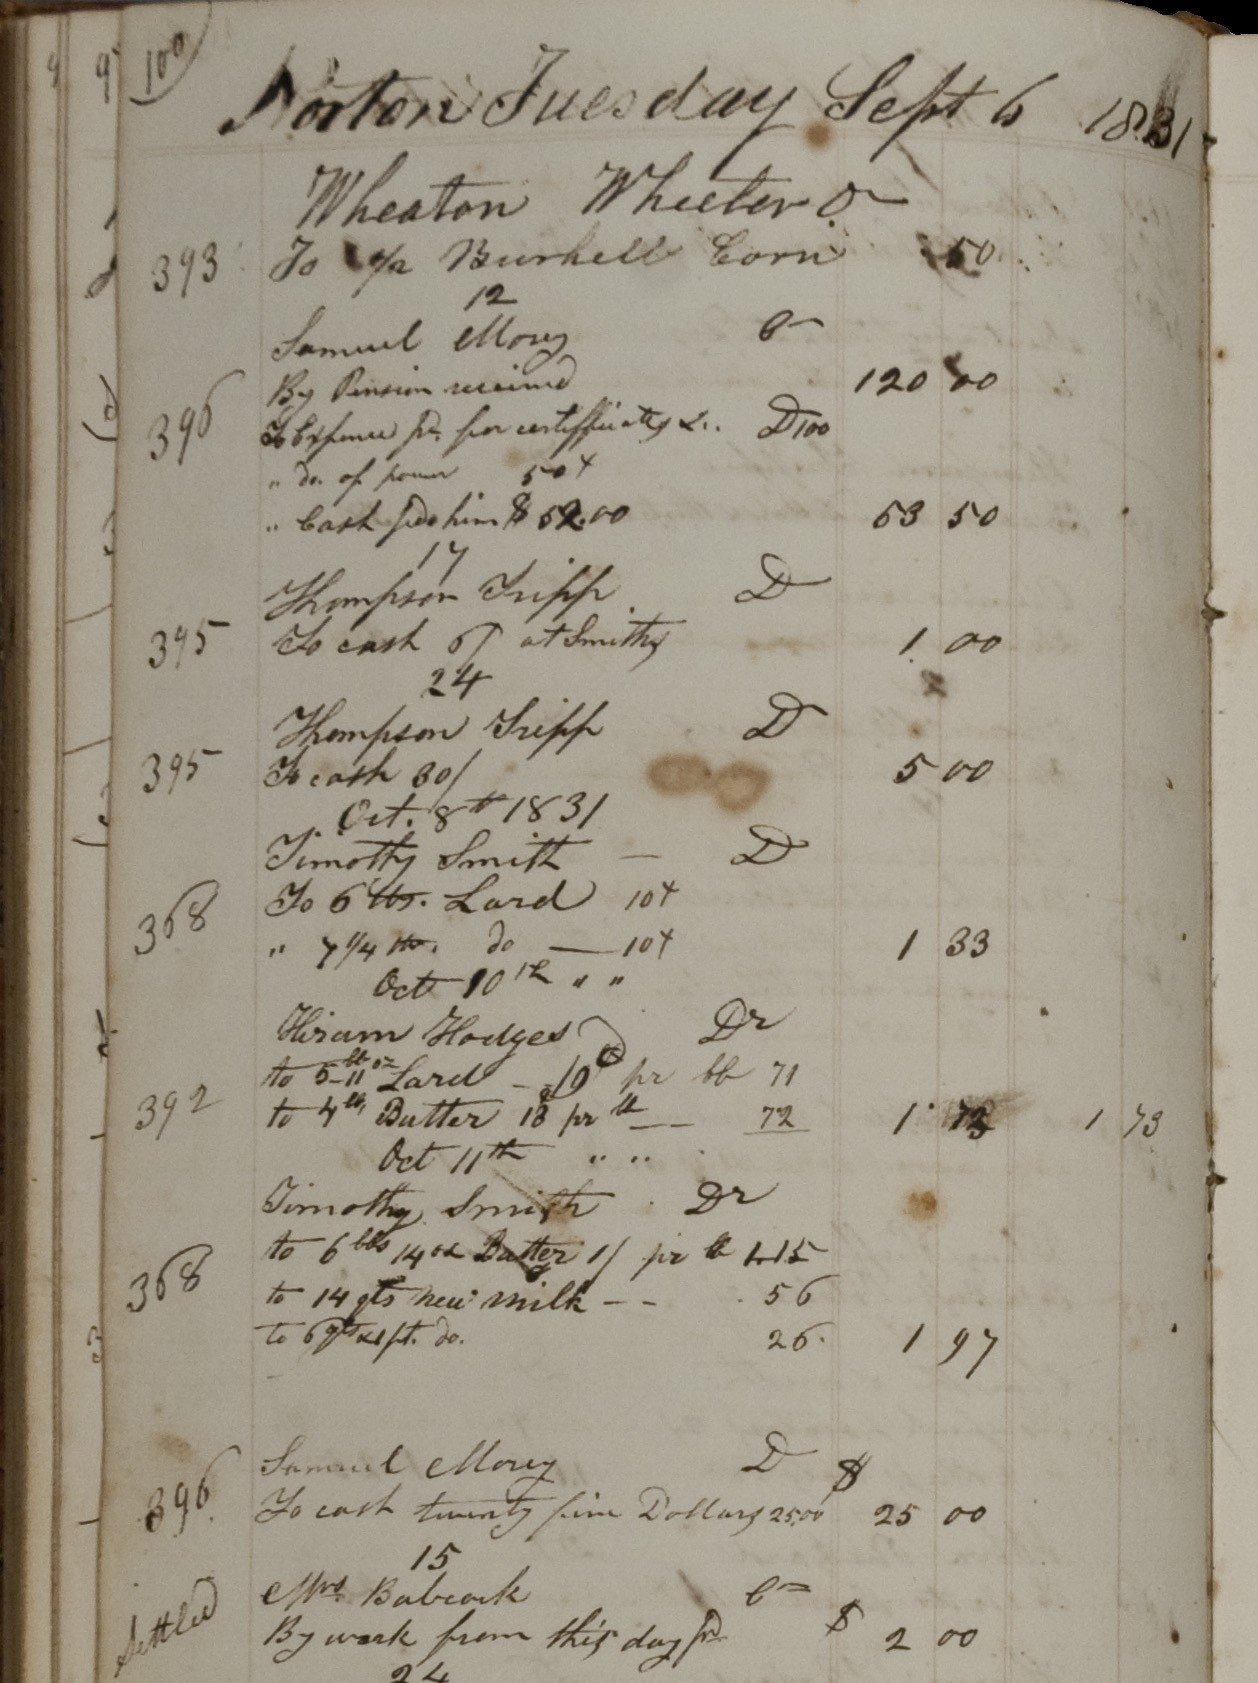
\includegraphics[width=1\textwidth]{img/wheaton_100_101.jpg}  
    \caption[Seite 100 des \textit{Daybook, \protect\url{hdl.handle.net/11040/17982}}, 1828-1859]{Seite 100 des \textit{Daybook}, 1828-1859a} \label{fig:wheaton}
\end{figure}
Die vollständige Transkription der ersten 8 Einträge der Seite 100. Diese zeigen die soeben beschriebenen Strukturen.
\\
\\
\begin{tabular}{clcc}
 \textbf{Norton Tuesday Sept 6 1831}\\
    & Wheaton Wheeler & &\\
393 & Dr To 1/2 Burhell Corn & & 50 \\
    & 12 & &\\
    & Samuel Morey  Cr  & &\\
396 & By pension received & 120 & \\
    & To Expense pd. for certificates L. D100 & &\\
    & "Do. of power 50x & &\\
    & " Cash pd. him \$62.00 & 53 & 50\\
    & Thompson Tripp  DR  & &\\
395 & To cash 6/ at Smiths & 1 & 00\\	
    & 24 & &\\
    & Thompson Tripp  DR & &\\	
395 & To cash 30/ & 5  & 00\\		
Oct. 8th 1831\\
    & Timothy Smith DR & &\\
368 & To 6 lb. Lard 10x 6 lb. Lard"7 1/4 lb do 10x & 1 & 33 \\
Oct 10th " "\\
    & Hiram Hodges Dr & &\\
392 & To 5 lb11 oz Lard - 19d pr lb\\
    & 71 5 lb11 oz Lard To 4 lb Butter 13 pr lb 72 & 1 & 73\\
Oct. 11th " "\\
    & Timothy Smith  Dr& &\\
368 & To 6 lbs 14 oz Butter 1/ pr lb 1.15 & & \\ & To 14 Qts New Milk 56 & &\\
& To 6 Qts \& 1 Pt. do 26 & 1 & 97 	\\	
    & Samuel Morey DR & &\\
396 & To cash twenty five dollares 25.00 & 25 & 00\\
    & 15 & & \\	
    & Mrs. Babcock DR  & & \\		
Settled & By work from this day pd & \$2 & 00
\end{tabular}
\medskip
\begin{center}
\textit{Transkription der Seite 100 des \textit{Daybook}}
\end{center}
TOMASEK verfolgt dabei einen TEI/XML-Ansatz, um die die textuelle Struktur der Quelle und die inhaltliche Struktur der Transaktionen zu beschreiben. Letztere ist schwerer durch reines TEI Markup beschreibbar bzw. für eine weiter Analyse schwere nachnutzbar, da man für eine algorithmische Auswertung diskrete Daten braucht.

\newpage
\textcolor{red}{
Das ''\textit{Slave-Ledger}'', das \textit{Daybook} eines Geschäftsmannes rund die Finanzaufzeichnung von George Washington lassen sich auf Grund der regionalen und zeitlichen Einordnung gut miteinander vergleichen und weisen ähnliche textuelle und semantische Strukturen auf. Ihre Kontextualisierung, sowie an die Quellen gestellten Forschungsfragen variieren, lassen sich aber auch wieder auf wiederkehrende Entitäten, wie Personen, Orte und Waren- bzw. Geldflüsse zurückführen. Um eine bessere maschinelle Analyse der Information in diesen Quellen zu ermöglichen, sowie historische Rechnungsunterlagen zu beschreiben, die eine andere Struktur aufweisen, bedarf es standardisierter Modelle. Im nächsten Kapitel wird eine Vorgehensweise und Technologie-Stack beschrieben, der dies ermöglicht.
}

\newpage
%%%%%%%%%%%%%%%%%%%%%%%%%%%%%%%%%%%%%%%%%%%%%%%%%%%%%%%%%%%%%%%%%
%%%%%%%%%%%%%%%%%%%%%%%%%%%%%%%%%%%%%%%%%%%%%
\section{Web of Data}
\label{WebofData}
Das \textit{Semantic Web}, oder wie es seit 2013 vom \textit{World Wide Web Consortium} (W3C) genannt wird, \textit{Web of Data} umfasst einen Stack an Standards und Technologien.\footnote{Linked Data, \url{w3.org/standards/semanticweb/data.html}, 23.11.2019} Dieser Stack dient dazu, Daten und ihre Struktur ausdrucksstark zu beschreiben, sodass Daten maschinenlesbar über das Web verteilt und genutzt werden können. Für die Geisteswissenschaften und die Geschichtswissenschaften im Speziellen eröffnet dieser Technologie Stack, dass Forschungsdaten ausführlich strukturiert, kontextsensitiv, sich selbst beschreibend, genutzt werden können.
\\
Dieses Kapitel dient dazu anfangs die Geschichte, die Idee des und Kritik am \textit{Web of Data} zu beschreiben, geht dann auf den Technologie Stack ein und setzt dann einen Schwerpunkt beim Bereich Ontologien. Diese Schwerpunktsetzung erfolgt, da Ontologien eine maschinenlesbare Umsetzung von Modellen ermöglichen und Kapitel \ref{Umsetzung} sich mit der sogenannten \textit{Bookkeeping Ontology} beschäftigt, die für das Mapping von historischer Information in historischen Rechungsbüchern verwendet wird.  

%%%%%%%%%%%%%%%%%%%%%%%%%%%%%%%%%%%%%%%%%%%%%
%%%%%%%%%%%%%%%%%%%%%%%%%%%%%%%%%%%%%%%%%%%%%
\subsection{Geschichte und Vision des \textit{Web of Data}}

''\textit{The Semantic Web will bring structure to the meaningful content of Web pages, creating an environment where software agents roaming from page to page can readily carry out sophisticated tasks for users.}''\footcite[][S.3]{berners2001semantic}
\\
\\
Beim \textit{TED Talk} im Jahre 2009 fordert Tim Burners-Lee das Auditorium auf, mit ihm gemeinsam die Worte zu rufen: ''\textit{Raw Data Now!}''.\footnote{BERNERS-LEE Tim: The Next Web, \url{ted.com/talks/tim_berners_lee_on_the_next_web?language=de}, 05.04.2019.} Die Vision von Burners-Lee, dem Erfinder des World Wide Web, ist das sogenannte \textit{Semantic Web}. Im Gegensatz zum klassischen Web, das als ein Web von Dokumenten betrachtet werden kann, versucht das \textit{Web of Data} Daten aus unterschiedlichen Quellen zu integrieren und miteinander zu verknüpfen. Daten sollen so vorliegen, dass nicht nur Menschen diese in neuen Kontexten nutzen können, sondern auch Softwareagenten. Maschinen sollen in der Lage sein selbständig die Struktur von Daten ''verstehen'' zu können, um bestimmte Aufgaben umsetzen zu können. Oder anders formuliert: Maschinen sollen in die Lage versetzte werden Inhalte im Web soweit selbstständig verarbeiten können, dass Automatisierung auf Ebene der Bedeutung möglich ist. Ein konkretes Anwendungsszenario, das mit Hilfe des \textit{Web of Data} umgesetzt wird sind verbesserte Suchfunktionalitäten für Informationssysteme, die auch die semantische Ebene miteinbeziehen. TOCHTERMANN und MAURER führen ein Beispiel eines Informationsbedürfnisses einer Person an, die gerne einen Termin mit einem Arzt in Graz vereinbaren möchte, der gleichzeitig auch ein Homöopath ist. Diese Person stellt eine Suchanfrage in einer dafür geeigneten Suchmaschine, bestehend aus 4 Wörtern: ''Ärzte, Homöopathie, Stadt Graz''. Da in einer klassischen Suchmaschine nur das Vorkommen der Wörter berücksichtigt wird, muss die suchende Person sich noch durch die angezeigten Suchergebnisse arbeiten, bis sie den passenden Treffer gefunden hat. Eine Suchmaschine im \textit{Web of Data} ist in der Lage sogenannte Wissensbasen zu befragen, um welche Begriffe es sich hinter den Zeichenketten handelt.\footcite[S.1-2]{pellegrini2006semantic} 
\\
Dabei handelt es sich aber weder um Maschinen die selbstständig lernen, oder gar eine künstliche Intelligenz, sondern um formalisiertes, maschinenlesbares Wissen.\footcite[S.1-6]{pellegrini2006semantic} Der Wissensbegriff in diesem Zusammenhang entspringt einer informationswissenschaftlichen Perspektive wie bei WERSIG\footcite{wersig1971information}, KUHLEN\footcite{weller2013InformationBand} oder FAUVR-BULLE\footcite{favre2001information} und sowie im Kapitel \ref{forschungdaten} und \ref{Ontologie} kurz angeführt.

%%%%%%%%%%%%%%%%%%%%%%%%%%%%%%%%%%%%%%%%%%%%%
\subsubsection{Kritik am \textit{Web of Data}}
\textcolor{red}{
''\textit{I will never touch that crap of RDF or the semantic web; this is a pipe dream of reality ignoring academics and I will not have it. I will only use JSON-LD.}''
\\
\\
Ist ein Zitat eines Vortrages von Phil ARCHER aus dem Jahr 2014. Viele IT-Entwickler sehen \textit{Web of Data} Standards kritisch und so ist das \textit{Semantic Web} nicht erreicht.\footcite{wettlaufer2018semanticwebEdition}} Zumindest nicht für die Allgemeinheit. Die großen Internetriesen hingegen verfügen über ihre eigene ''Semantic Web'', in denen sie ihre eigenen Agenten mit ihrer großen Datenmenge arbeiten lassen. So verwendet Google beispielsweise seinen \textit{Knowledge Graph}, um Ergebnisse für Suchanfragen zu verbessern.\footnote{Whatever Happened to the Semantic Web? , \url{twobithistory.org/2018/05/27/semantic-web.html}}
\\
Auf der anderen Seite gibt es aber einige Stimmen, die das \textit{Web of Data} in ihrer jetzigen Überlegung kritisieren und es wurde schon vor Jahren als Zukunfsttechnologie totgesagt. Die Kritik richtet sich daran, dass die Überlegungen zu akademisch und technisch zu kompliziert sein. SHIRKY kritisiert, dass der top-down Ansatz, die unflexible, strenge Art der Formalisierung und die zu starke Spezifikation auf einzelne Domänen von Ontologien nicht sinnvoll in einem dezentralen Web funktionieren können.\footcite{shirky2005ontology} Die Kritik von SWARTZ, der sich ein \textit{Semantic Web} herbeisehnt, richtet sich an den, in seinen Augen noch nicht ausgereiften, Technologie Stack und die zu komplizierten und aufdröselten Standards. Beispielsweise ist für SWARTZ XML im Gegensatz zu JSON zu überladen und kann nur mir mehr Aufwand verarbeitet werden.\footcite{swartz2013aaron}
\\
Festzuhalten ist aber, dass im Aufkommen der AI-Forschung, der Künstlichen Intelligenz, Themen wie \textit{Knowledge Graphs} und Wissenbasen, und so auch das \textit{Semantic Web}, wieder interessanter werden. Sie helfen dabei AI-Algorithmen und Entscheidungen zu unterstützen und dabei ''Bedeutung'' in großen Mengen an Text zu extrahieren und zu formalisieren.\footcite[][]{bernstein2016new}


\newpage
%%%%%%%%%%%%%%%%%%%%%%%%%%%%%%%%%%%%%%%%%%%%%
%%%%%%%%%%%%%%%%%%%%%%%%%%%%%%%%%%%%%%%%%%%%%
\subsection{Web of Data Stack}

Um diese Vision in die Tat umzusetzen bedarf es mehrerer aufeinander aufbauender, technischer Grundlagen, die sich im \textit{Semantic Web Stack} manifestieren.
In Abbildung \ref{fig:webstack} werden die Technologien und Standards des \textit{Web of Data} im sogenannten \textit{Semantic Web Stack} dargestellt.
\begin{figure}[h]
  \centering
	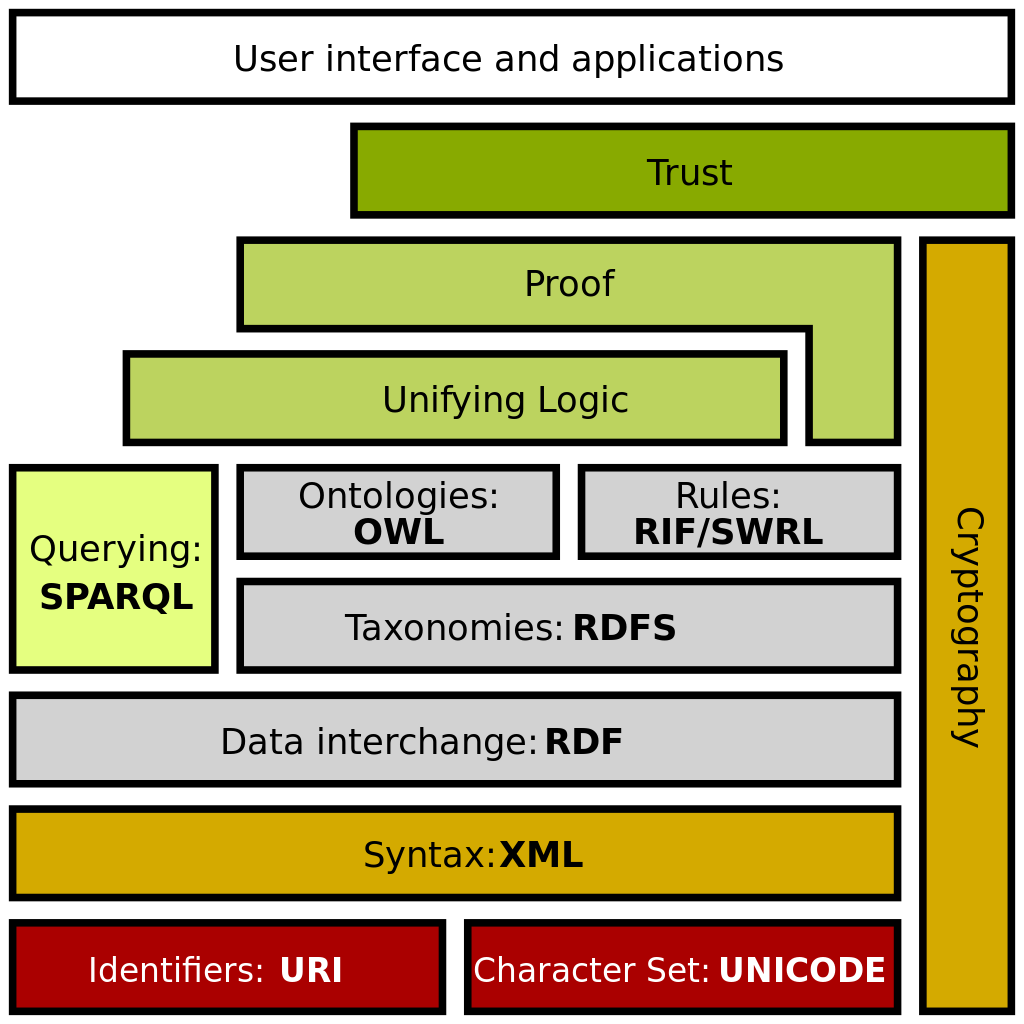
\includegraphics[width=0.7\textwidth]{img/web_stack.png}  
    \caption[Semantic Web Stack, \protect\url{en.wikipedia.org/wiki/Semantic_Web_Stack}, 29.12.2019.]{Semantic Web Stack}
  	\label{fig:webstack}
\end{figure}
Es gibt unterschiedliche Darstellungen dieses Stacks, dennoch zeigt diese Version alle grundlegende Konzepte. Der \textit{Web of Data Stack} ist von unten nach oben zu lesen. In den Kästchen in denen eine Abkürzung, wie URI oder RDF, angeführt werden, sind Technologien bereits im Einsatz. Die Themen \textit{Trust}, \textit{Proof} etc. sind noch Bestandteil gegenwärtiger Forschung. Grob zusammengefasst beschreiben diese Konzepte, wie eine vertrauenswürdige und 'wahre' Kommunikation zwischen Akteuren im \textit{Web of Data}, sowie die Verschlüsselung und Anwendung sichergestellt werden kann. 
\\
Die Basis des Stacks bilden \textit{Uniform Resource Identifier} (URI), die Ressourcen im Web eindeutig identifizieren und \textit{UNICODE} als internationaler Standard zur Zeichenkodierung. Der Syntax Bereich wird mit der \textit{Extensible Markup Language} (XML), einer Auszeichnungssprache zur Strukturieren von Text, ermöglicht, wobei diese Technologie immer mehr durch die \textit{JavaScript Object Notation} (JSON) ersetzt wird. Das \textit{Resource Description Framework} dient dazu Daten im Web auszutauschen und ermöglicht es Daten als Graphen zu beschreiben. Die formalen Regeln für RDF werden mittels \textit{Resource Description Framework Schema} RDFS und \textit{Web Ontology Language} (OWL) beschrieben. RDFS erlaubt es Klassen und Beziehungen zwischen Klassen zu beschreiben und OWL ermöglicht es weitere logische Regeln in Modellen abzubilden. \textit{SPARQL Protocol And RDF Query Language} (SPARQL) ist, vergleichbar mit SQL in der relationalen Datenbankwelt, die graphenbasierte Abfragesprache für RDF Daten.\footcite[][]{horrocks2005semantic}
\\
In den folgenden Unterkapiteln werden nun die angeführten Technologien weiter beschrieben. Die Konzepte ohne Technologien, sowie \textit{RIF/SWRL}, werden dabei, da sie für diese Arbeit nicht essentiell sind, nicht behandelt.


%%%%%%%%%%%%%%%%%%%%%%%%%%%%%%%%%%%%%%%%%%%%%
%%%%%%%%%%%%%%%%%%%%%%%%%%%%%%%%%%%%%%%%%%%%%
\subsubsection{Daten als Graph: Resource Description Framework}

RDF ist ein Datenmodell zur Darstellung und für den Austausch von Daten im Web. Daten werden in diesem Modell als Ressourcen definiert, wobei eine Ressource alles sein kann: ein Dokument, eine Person, ein physisches Objekt oder ein abstraktes Konzept. Über Ressourcen werden Statements der Form Subjekt-Prädikat-Objekt formuliert. Jedes Statement drückt eine Beziehung zwischen zwei Ressourcen aus. Das Subjekt und das Objekt stehen dabei für die beiden miteinander verbundenen Ressourcen; das Prädikat beschreibt die Art ihrer Beziehung. Diese Zusammensetzung von Subjekt, Prädikat und Objekt werden als Triples bezeichnet. Betrachtet man den Satz ''\textit{Bob ist befreundet mit Alice}'', dann lässt sich folgendes Triple extrahieren: \textit{<Bob>} als Subjekt, \textit{<ist befreundet mit>} als Prädikat und \textit{<Alice>} als Objekt. Ob \textit{Alice} mit \textit{Bob} befreundet ist, geht aus diesem Statement noch nicht hervor, da jeder Relation in RDF nur eine Richtung definiert.\footcite[][S.16-21]{powers2003practical} In der graphischen Darstellung wird schnell klar, dass es sich beim RDF Datenmodell um einen gerichtete Graphen handelt, der aus Knoten (Subjekt und Objekt), sowie aus Kanten (Prädikat) besteht, wie Abbildung \ref{fig:triple} zeigt.
\begin{figure}[H]
  \centering
	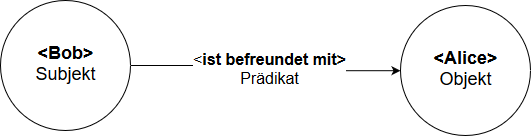
\includegraphics[width=0.75\textwidth]{img/triple.png}  
    \caption[Beispiel eines Tripel]{Beispiel eines Tripel, eigene Darstellung, 17.07.2019}
  	\label{fig:triple}
\end{figure}
SCHREIBER und RAIMOND\footcite[][]{schreiber2014rdf} erklären RDF in einem ausführlichen Beispiel an Hand folgenden Aussagen:
\\
\\
\textit{Bob ist eine Person.\\
Bob ist befreundet mit Alice.\\
Bob ist geboren am 4. Juli 1990. \\
Bob interessiert sich für die Mona Lisa.\\
Die Mona Lisa wurde von Leonardo da Vinci entworfen.}
\\
\\
Jede dieser Zeilen steht für ein Triple. \textit{Bob} ist Subjekt in vier der oben genannten Tripeln, \textit{Mona Lisa} tritt zweimal als Objekt und einmal als Subjekt auf. Dies ermöglicht es eine beliebige Menge an Triple zu einem komplexeren Graphen zusammenzusetzen und somit komplexere Sachverhalte beschreiben zu können. Abbildung \ref{fig:rdf_example} veranschaulicht das.
\begin{figure}[H]
  \centering
	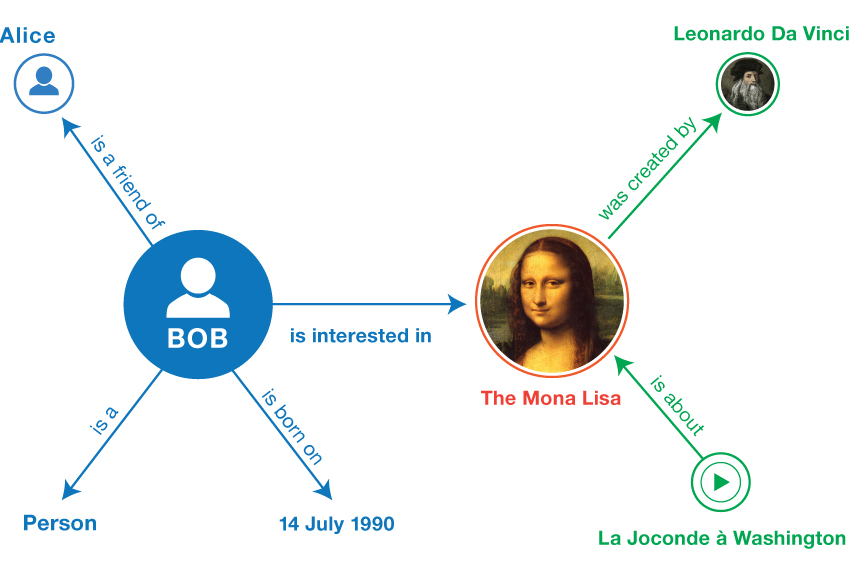
\includegraphics[width=1\textwidth]{img/rdf_example.png}  
    \caption[Visualisierung eines Graphen auf Basis eines RDF-Datensatz, w3.org/TR/rdf11-primer, 10.04.2019.]{Visualisierung eines Graphen auf Basis eines RDF-Datensatz.}
  	\label{fig:rdf_example}
\end{figure}
\textbf{URI} können in allen drei Positionen eines Triple erscheinen. Somit ist jeder Ressource, sowie jeder Beziehung zwischen Ressourcen durch eine URI identifizierbar. URI's sind durch ein erweiterbares Schema definiert, damit Ressourcen im Internet eindeutig adressiert werden können. Um dabei die Einheitlichkeit zu gewährleisten, folgen sie einem vordefinierten Satz von Syntaxregeln, der 5 Komponenten beinhaltet:\footcite[][]{berners2004uniform}
\begin{center}
\textit{URI = scheme:[//authority]path[?query][\#fragment]}
\\
\end{center}
\begin{itemize}
\item \textbf{\textit{scheme}}: Definiert den Kontext und Typ. Bekannte Schemata sind die Webprotokolle \textit{Hyper Text Transfer Protocol} (HTTP) oder das \textit{File Transfer Protocol} (FTP), sowie Notationskonzepte wie \textit{Uniform Resource Name} (URN) oder \textit{Digital Object Identifier} (DOI).
\item \textbf{\textit{authority}}: Verwaltet Instanzen in einem vom Schema definierten Interpretationsraum. Ein Beispiel ist das \textit{Domain Name System}, wie etwa \textit{gams.uni-graz.at}
\item \textbf{\textit{path}}: Der Pfad enthält – oft hierarchisch organisierte – Angaben, die zusammen mit dem Abfrageteil eine Ressource identifizieren und beschreibt den Weg durch die Filestruktur auf einem Server zu einem Dokument.
\item \textbf{\textit{query}}: Der Abfrageteil beinhaltet Daten zur Identifizierung von solchen Ressourcen, deren Ort durch die Pfadangabe allein nicht genau angegeben werden kann, wie beispielsweise ein Datensatz aus einer Datenbank.
\item \textbf{\textit{fragment}}: Ist der optionale Fragmentbezeichner und referenziert eine Stelle innerhalb einer Ressource. Der Fragmentbezeichner bezieht sich immer nur auf den unmittelbar vorangehenden Teil des URI und wird von einem Hash (\#) eingeleitet und entspricht oft einer ID in einem HTML Dokument.
\end{itemize}

Weiters werden URI in \textbf{\textit{Uniform Resource Locator}} (URL) und \textbf{\textit{Uniform Resource Name}} (URN) unterteilt. Wo URN Namen von Ressourcen eindeutig identifizieren, wie etwa bei ISBN Nummern von Büchern, sind URL die gängigsten URI's, die den Ort einer Ressource adressieren und über einen Webbrowser auch aufrufen können.\footcite[][S.21-22]{powers2003practical} Für das Triple \textit{<Bob>} \textit{<interessiert sich für>} \textit{<die Mona Lisa>} wird jeder Teilbestand eine URI und in der \textit{Turtle} Serialisation von RDF ergibt es folgenden Code:
\begin{lstlisting}[]
BASE <http://example.org/>
PREFIX foaf:<http://xmlns.com/foaf/0.1/>
PREFIX xsd:<http://www.w3.org/2001/XMLSchema#>
PREFIX schema:<http://schema.org/>
PREFIX dcterms:<http://purl.org/dc/terms/>
PREFIX wd:<http://www.wikidata.org/entity/>

bob#me a foaf:Person ;
          foaf:knows <alice#me> ;
          schema:birthDate "1990-07-04"^^xsd:date ;
          foaf:topic_interest wd:Q12418 .
 
wd:Q12418 dcterms:title "Mona Lisa" ;
           dcterms:creator <http://dbpedia.org/resource/Leonardo_da_Vinci> .
\end{lstlisting}

\textit{BASE} und \textit{PREFIX} definiert die Namespaces, die als Kurzschreibweise für die \textit{authority} in der URI verwendet werden und jeweils auf ein RDF oder OWL verweisen. Jede Zeile entspricht nur der Formalisierung eines Tripels. Überall stehen URIs, mit Ausnahme von ''1990-07-04'' und ''Mona Lisa''. Hierbei handelt es sich um Literale, die bestimmte Datentypen, einmal ein Datum und einmal reinen Text, umfassen. 
\\
Verbalisiert bedeutet der Code folgendes: eine Person (bob\#me) aus der \textit{Friend of a Friend} (FOAF) Ontolgie kennt eine andere Person (<alice\#me>). Weiters hat die ein Geburtsdatum in Form eines normalisierten Datums und ist interessiert an dem Thema (wd:Q12418). Dieses Thema wird nun weiters beschrieben und es handelt sich dabei um den Datensatz zur Mona Lisa in Wikidata, einer freien und offenen Wissensbasis, die von Menschen und Maschinen befüllt und verwaltet wird.\footnote{Wikidata, \url{wikidata.org}, 04.01.2019.}
%%%%%%%%%%%%%%%%%%%%%%%%%%%%%%%%%%%%%%%%%%%%%
%%%%%%%%%%%%%%%%%%%%%%%%%%%%%%%%%%%%%%%%%%%%%
\subsubsection{Klassen und Beziehungen: Resource Description Framework Schema (RDFs)}

Im vorhergehenden Beispiel wurden \textit{<Bob>} und \textit{<Alice>} der Klasse \textit{<Person>} zu geordnet. Sie sind Instanzen der Klasse \textit{<foaf:Person>}. Desweiteren wurde eine Relation zwischen diesen beiden Personen definiert: \textit{Bob ist befreundet mit Alice}.
\\
Um die Beziehungen zwischen Ressourcen zu beschreiben, liefert das \textbf{Resource Description Framework Schema (RDFs)}\footcite[][]{brickley2014rdf} eine semantische Erweiterung für RDF. Dies umfasst die Möglichkeit Klassen und Relationen, sogenannte Properties, zu definieren und folgt dem Paradigma der Objektorientierung. Es lassen sich auf diese Weise Instanzen von Klassen erzeugen, die alle Eigenschaften der Klasse und ihrer übergeordneten Klassen erben. Blickt man auf das FOAF-Vokabular\footnote{FOAF-Specification, \protect\url{xmlns.com/foaf/spec/ }, 29.05.2019.}, das als RDFs umgesetzt ist, so kann man feststellen, dass \textit{foaf:Person} eine Unterklasse von \textit{foaf:Agent} ist. Weitere Unterklassen davon sind \textit{foaf:Group} und \textit{foaf:Organization}. Alle drei Unterklassen haben bestimmte Eigenschaften gemeinsam: sie setzen Handlungen in der Welt. Sie unterscheiden sich aber in den Relationen mit denen sie selbst, oder in Abgrenzung zu anderen Klassen, beschrieben werden können. Eine \textit{foaf:Group} besteht aus mehreren \textit{foaf:Person}. Dies wird mittels der Property \textit{foaf:member} ausgedrückt. Im Gegenzug verfügt \textit{foaf:Person} über eine Relation \textit{foaf:knows}, die ausdrückt, dass sich zwei Personen kennen. Die Richtung dieser Relation - wer wen kennt - wird mit den in RDFs mittels den Termen \textit{rdfs:Domain} und \textit{rdfs:Range} definiert. 
Für \textit{foaf:knows} wird \textit{Domain} und \textit{Range} auf die Klasse\textit{ foaf:Person} gesetzt: eine Person kennt eine andere Person. Für die Property \textit{foaf:member} wird \textit{Domain} auf \textit{foaf:Group} und \textit{Range} auf \textit{foaf:Person} gesetzt: eine Gruppe besteht aus Personen.
\\
Weiter führt RDFs Datentypen ein. Damit lässt sich beschreiben, um welche Art eines Literals es sich handelt. Es kann für die maschinelle Verarbeitung sehr wichtig sein zu wissen, ob es sich um eine Zeichenkette, eine Zahl, eine Datumsangabe oder eine XML Struktur handelt, da mit unterschiedlichen Datentypen andere Operationen einhergehen. 
\\
Mit den RDF Properties \textit{rdfs:label} und \textit{rdfs:comment} lassen sich Properties und Classes benennen und beschreiben. Das ist deswegen nötig, da der Fokus einer Klasse nur in bestimmten Kontexten Sinn macht. \textit{rdfs:label} definiert einen menschenlesbaren Namen einer Ressource. Es besteht stets die Möglichkeit in RDF die einzelnen Lables einer Ressource mit Sprachkürzel zu versehen. Die Property \textit{rdfs:comment} erlaubt es eine verbale Beschreibung zu einer Klasse hinzuzufügen. Am Beispiel von \textit{foaf:Person} ist das das Label ''Person'' und die Beschreibung:
\\
\\
'\textit{The Person class represents people. Something is a Person if it is a person. We don't nitpic about whether they're alive, dead, real, or imaginary. The Person class is a sub-class of the Agent class, since all people are considered 'agents' in FOAF. }''.
\\
\\
Daneben existiert auch ein Konstrukt \textit{rdfs:seeAlso}, um ausdrücken, dass es unter folgender URL noch weitere Information zu dieser Ressource gibt.\footcite{brickley2014rdf} Folgende Darstellung veranschaulicht die soeben beschriebenen Konstrukte in RDFs und zeigt Unterklassen der Superklasse \textit{foaf:Agent}, zwei Instanzen der Klasse \textit{foaf:Person} und stellt graphisch - durch den Pfeil - \textit{Domain} und \textit{Range} einer Property dar.\footcite[][S.33-88]{hitzler2007semantic}  
\begin{figure}[H]
  \centering
	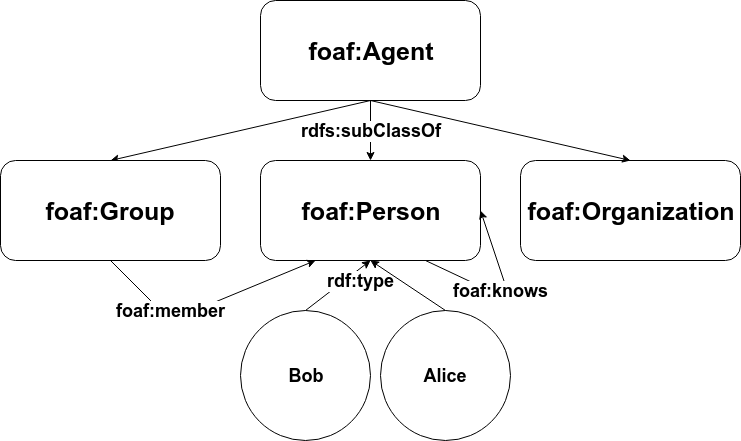
\includegraphics[width=0.75\textwidth]{img/rdfs.png}  
    \caption[RDFs-Beispiel auf Basis des FOAF-Vokabulars, eigene Darstellung.]{RDFs-Beispiel auf Basis des FOAF-Vokabulars}
  	\label{fig:rdf}
\end{figure}
Hinter jeder Klasse, Property und jeder Instanz steht eine URI. Folgendes RDF-Snippet zeigt wie die Klasse \textit{foaf:Person} und \textit{foaf:knows} im FOAF-Vokabular mittels RDFs definiert werden.


\begin{lstlisting}[]
PREFIX rdfs:<http://www.w3.org/2000/01/rdf-schema#> .
PREFIX foaf:<http://xmlns.com/foaf/0.1/>
PREFIX rdf:<http://www.w3.org/1999/02/22-rdf-syntax-ns#> .

foaf:Person a rdfs:Class ;
  rdfs:label "Person" ;
  rdfs:comment "A person." ;
  rdfs:subClassOf foaf:Agent .
  
foaf:knows a rdf:Property;
  rdfs:label "knows" ;
  rdfs:comment "A person known by this person (indicating some 
  level of reciprocated interaction between the parties)." ;
  rdfs:domain foaf:Person ;
  rdfs:range foaf:Person .
\end{lstlisting}


%%%%%%%%%%%%%%%%%%%%%%%%%%%%%%%%%%%%%%%%%%%%%
%%%%%%%%%%%%%%%%%%%%%%%%%%%%%%%%%%%%%%%%%%%%%
\subsubsection{Abfragesprache: SPARQL}
Wie man in der Welt der relationalen Datenbanken mit der Abfragesprache SQL Datenbankabfragen formulieren kann, so kann man mit \textit{SPARQL Protocol And RDF Query Language} RDF Daten bzw. Triple in Graphdatenbanken abfragen.\footcite[][]{w3c2013sparql}
\\
Folgendes Snippet einer SPARQL-Abfrage zeigt die Syntax dieser Abfragesprache. Ziel dieser Abfrage ist es, alle Ressourcen in einer Graphdendatenbank abzufragen, die über eine \textit{foaf:name} und eine \textit{foaf:knows} Property verfügen. Das Ergebnis wird nach den Personen und Namen gruppiert, also es werden keine Dubletten von URI's zurückgegeben. Als Ausgabe erfolgt eine Tabelle (im XML, JSON oder CSV Datenformat) in der die Namen und die Anzahl der Freunde, definiert als alle Knoten auf die \textit{foaf:know} referenziert.
\begin{lstlisting}[]
PREFIX foaf: <http://xmlns.com/foaf/0.1/>
SELECT ?name (COUNT(?friend) AS ?count)
WHERE { 
    ?person foaf:name ?name . 
    ?person foaf:knows ?friend . 
} 
GROUP BY ?person ?name
\end{lstlisting}
Mit PREFIX werden die Namespaces definiert. Das reservierte Wort \textit{SELECT} definiert alle Variabeln. Diese werden durch ein vorangestelltes Fragezeichen gekennzeichnet, die als Rückgabewert definiert werden. Daneben gibt es in der Version 1.1 von SPARQL Operatoren und Funktionen, wie etwas \textit{COUNT()}, das alle Treffer der \textit{?friend} Variabel zählt und in der \textit{?count Variabel} speichert. Im \textit{WHERE} Bereich werden alle Bedingungen für die Abfrage definiert. Diese Bedinungen entsprechen der Definition eines Teilgraphen, der wiederum eine Teilmenge des gesamten Datenbestandes abbildet. Hier stehen weiter Konstrukte wie \textit{OPTIONAL}, einem logischen Oder, so wie \textit{UNION} einem logischen Und zur Verfügung. Über eine SPARQL-Endpoint können so User über das Web Datenbestände abfragen und mit diesen arbeiten.\footcite[][S.1-45]{ducharme2013learning}


%%%%%%%%%%%%%%%%%%%%%%%%%%%%%%%%%%%%%%%%%%%%%
%%%%%%%%%%%%%%%%%%%%%%%%%%%%%%%%%%%%%%%%%%%%%
\subsection{Formalisierung von Modellen: Ontologien}
\label{Ontologie}

Der Gegenstandsbereich der \textbf{Ontologie als Disziplin in der Philosophie} umfasst alles, das existiert. Das Erkenntnisziel, so MEIXNER, ist auf allgemeiner begrifflicher Ebene zu finden und beschäftigt sich mit der Einteilung des Seins und den Grundstrukturen der Wirklichkeit, sowie der Frage nach dem Wesen der Existenz. Die Ontologie verfolgt nicht das Ziel Erkenntnis über ein Objekt zu erhalten, es beispielsweise zu vermessen oder zu beschreiben, sondern stellt sich die Frage nach welchen allgemeinen Kriterien Objekte im Verhältnis zu ontologischen Begriffen wie Sein, Aktualität, Universalie, Exemplifikation, Sachverhalt oder Individuum stehen.\footcite{meixner1994wissenschaft}
\\
Der Begriff \textbf{Ontologie in der Informationswissenschaft bzw. Informatik} umfasst ein pragmatisches Konzept zum Austausch und zur Wiederverwendung von formalisierten und gemeinschaftlich verwendeten Wissensstrukturen durch ein gemeinsames Vokabular. Ziel dabei ist es, Informationssysteme zu implementieren. Die Spezifikation eines solchen Vokabulars für eine bestimmte Domäne, ob übergeordnet und generalisierend , oder fachspezifisch, nennt man Ontologie.
\\
Der Begriff wird in zwei Disziplinen mit jeweils unterschiedlichem Fokus verwendet. Dennoch können Gemeinsamkeiten festgemacht werden. Beide setzen sich mit der Frage auseinander, wie die Welt sinnvoll strukturiert werden kann, damit wir uns besser darin zurecht finden können. In diesem Kapitel wird die informationswissenschaftliche Dimension des Ontologie-Begriffs und seiner Nutzung in den digitalen Geisteswissenschaften diskutiert und der Frage nachgegangen, ob Ontologien ein geeignetes Werkzeug zur Formalisierung von geschichtswissenschaftlichen Domänen darstellen. Dabei soll anfangs "Wissen" kurz aus informationswissenschaftlicher Sicht definiert werden und über das semantische Netz eine Brücke zur Ontologie geschlagen werden. 

%%%%%%%%%%%%%%%%%%%%%%%%%%%%%%%%%%%%%%%%%%%%%
%%%%%%%%%%%%%%%%%%%%%%%%%%%%%%%%%%%%%%%%%%%%%
\subsubsection{Vom Wissen, über das Semantische Netz zur Ontologie}

"\textit{An ontology is an explicit specification of a conceptualization}
"\footcite[][S.69]{hoekstra2009ontology}
\\
\\
\textbf{Wissen} ist eine systeminterne Repräsentation vorliegender Erfahrungen eines kognitiven Agenten zu einer bestimmten Zeit, die einem zu überprüfenden Anspruch auf Gültigkeit ausgesetzt sein muss. Wissen prägt das Handeln und Denken eines Agenten auf den unterschiedlichsten Ebenen und dient zur Lösung von Problemen im weitesten Sinne. Das jeweils aktuelle Wissen bildet einen kontextuellen Rahmen, in dem bestehende und ankommende Information interpretiert und zu neuen Erfahrungen verarbeitet werden.\footcite{favre2001information}
\\
Diese Definition von Wissen -- eine stärker informationswissenschaftliche -- hat seinen, neben vielen Definitionen in anderen Fachbereichen, legitimen Ursprung. Unterschiedliche Disziplinen haben andere Fragestellungen und benötigen dafür ein anderes theoretisches Gerüst. Ein Wissensbegriff in der Philosophie, beispielsweise, ist weiter gefasst, als ein Wissensbegriff in der Informationswissenschaft, dessen Aufgabe darin besteht als Hilfsmittel in der Entwicklung und Umsetzung von Informationssystemen zu fungieren. 
\\
\\
Mittels Ontologie lässt sich ''Wissen'' als Netzwerk beschreiben. Ein Netzwerk ist ein gerichteter Graph, bestehend aus einer Menge von Knoten und einer Menge von Kanten, die die einzelnen Knoten miteinander verknüpfen. Damit lassen sich (fast) beliebige Entitäten und deren Verknüpfungen miteinander abbilden. Die Überlegungen zu einem \textbf{semantischen Netz}, als gedanklichen Vorgänger der Ontologie, stammen von QUILIIAN, der damit ein formales Erklärungsmodell für '\textit{die menschliche Repräsentation von Wissen über Worte und ihre Bedeutung als Netzwerk von Begriffen und ihren Relationen}' \footcite{stuckenschmidt2009ontologien} beschreibt. Semantische Netze können einen Kompromiss zwischen menschenverständlicher Repräsentation einer Domäne  und der formalen Verarbeitbarkeit durch eine Maschine darstellen.\footcite{reichenberger2010grundlagen} Das ist dadurch gegeben, dass die Struktur des Graphen (= Netz), sich einfach in Rechnern als Matrizen abbilden lassen. Dies entspricht den Erörterungen von informellen Modellen in Kapitel \ref{Modell_def}.
\\
Die Ontologie ist eine Erweiterung des semantischen Netzes und nach GRUBER kann sie durch ein \textbf{4-Tupel} definiert werden. C ist eine Menge von \textbf{Klassen} (concepts, classes - Mengen von Entitäten aus der Realität), R eine Menge von \textbf{Relationen} (properties - Beziehungen zwischen Klassen), I eine Menge von \textbf{Instanzen} (individuals - einzelne Entität aus einer Menge) und A eine Menge von \textbf{Axiomen} (axioms - logische Regel).\footcite{joostbreukera2009flood} C und R lassen sich dabei stets als Graph abbilden. Ein Beispiel zur Veranschaulichung: 
\\
Es existiert eine Klasse (C) ''Katzen'', die mit der Relation ''ist ein'' (R) mit einer Klasse ''Säugetier'' verbunden ist.  Die Individuals (I) ''Garfield'' und ''Tom'' sind Instanzen der Klasse ''Katzen'' und erben alle Eigenschaften, die in der Klasse ''Katzen'' definiert wurden. Eine Regel kann definiert werden (A), sodass immer wenn eine Klasse eine ''ist ein'' Verbindung zu einer Klasse wie ''Säugetier'' hat, es ausgeschlossen ist, dass es eine zweite ''ist ein''-Verbindung  gibt, die auf eine andere Klasse wie etwa ''Vögel'' referenziert. 
\\
\\
Der Begriff der Ontologie wird terminologisch unscharf verwendet.\footcite[][S.1]{gruber1993translation} Zwar sind die Unterschiede klein, aber sind sie dennoch entscheidend und sollen im Folgenden diskutiert werden.
Eine der ersten Definitionen des Begriffs der Ontologie stammt von GRUBER: "\textit{An ontology is an explicit specification of a conceptualization}"
\\
Eine ''\textit{conceptualization}'' beschreibt den Prozess einer Vereinfachung, aber Fokussierung, eines bestimmten Aspekts der Realität. So kann eine Ontologie als Dokumentation eines wissenschaftlichen 
Prozesses agieren, in dem die Wirklichkeit abstrahiert und reduziert wird und gleichzeitig die Domäne bzw. Forschungsfrage hervorgehoben und amplifiziert wird.\footcite[][]{thaller2017ungefahre}
Unter ''\textit{explicit}'' versteht man, dass die Bedeutungen aller von der Ontologie erfassten Begriffe klar und eindeutig definiert sein müssen. Dies beinhaltet alle ihre Eigenschaften, Beschränkungen und Beziehungen, innerhalb, als auch außerhalb der Domäne.\footcite{sure2003methodology}
BORST erweitert GRUBERS Definition um  ''\textit{formal specification of a shared  conceptualization}''.\footcite{borst1997construction}
''\textit{Formal}'' ergänzt dabei die Definition um die Notwendigkeit, dass Ontologien maschinenlesbar sein müssen. Erst diese Eigenschaft hebt sie von anderen Methoden zur Formalisierung von konzeptionellen Datenmodellen hervor. Der Zusatz ''\textit{shared}'' reflektiert die Tatsache, dass eine Ontologie Wissen erfasst, das durch den Konsens einer Gruppe - z.B. durch einen wissenschaftlichen Diskurs - akzeptiert wird. Eine Ontologie sollte nicht im Stillen von einer Person alleine entwickelt werden, sondern in einem iterativen Prozess (\textbf{Ontology Engineering}) des Austausches und der Diskussion mit anderen entstehen. Ein solcher Prozess kann wie folgt ablaufen:
\begin{itemize}
\item Definition der Notwendigkeit und des Zieles einer Ontologie
\item Strukturierung des Wissens und konzeptionelle Entwicklung
\item Implementierung und Modellierung
\item Evaluierung und Dokumentation
\item Iteration dieses Prozesses im Austausch mit anderen
\end{itemize}
Allgemeiner betrachtet definieren LINCKELS \& MEINEL eine Ontologie als ein Datenmodell zur Darstellung eines Sets miteinander vernetzter Konzepte innerhalb einer (Fach-)Domäne.\footcite{linckels2011librarian} WELLER spricht von einer formalen und schematischen Darstellung einer Wissensdomäne auf Basis definierter Regeln und Vokabulars.\footcite{weller2013InformationBand}
\\ 
Zusammengefasst kann gesagt werden, dass sich mittels Ontologien komplexere Sachverhalte so darstellen lassen, dass Mensch und Maschinen in der Lage sind Strukturen, die durch eine Ontologie definiert und standardisiert sind, weiterverarbeiten zu können. Der Mehrwert kann vor allem in der Möglichkeit automatisierter Schlussfolgerungen, im Information Retrieval oder anderen formalen Methoden zur Verarbeitung von Daten liegen.\footcite[][S.162-178]{jannidis2017digital} 

\subsubsection{Reasoning}

Der Ontology Editor Protégé erlaubt es, eine Ontologie und die darin enthaltenen Daten (Individuals) einem Reasoning - dem Abarbeiten aller vorhandenen Regeln in einer Ontologie auf Basis einer deskriptiven Logik - zu unterziehen. Für solche Zwecke gibt es natürlich auch API's und Bibliotheken in Programmiersprachen.\footcite{musen2015protege} Das Reasoning gilt als ein essentieller Baustein im Design, der Entwicklung, der Wartung und in der praktischen Anwendung einer Ontologie. Das Ergebnis davon sind Inferenzen. Inferenzen sind neu hergeleitete Schlussfolgerungen auf Basis der formalen Regeln einer Ontologie.\footcite{dentler2011comparison} Die Überprüfung strukturierter Daten mittels logischen Schlussfolgerungen kann dazu dienen, größere Datenmengen auf ihre Konsistenz und somit auch auf ihre Qualität hin zu prüfen, da logische Inkonsistenzen als Fehlermeldung angezeigt werden.

%%%%%%%%%%%%%%%%%%%%%%%%%%%%%%%%%%%%%%%%%%%%%
%%%%%%%%%%%%%%%%%%%%%%%%%%%%%%%%%%%%%%%%%%%%%
%%%%%%%%%%%%%%%%%%%%%%%%%%%%%%%%%%%%%%%%%%%%%
\newpage
\section{Anwendung formaler Methoden auf Basis einer Ontologie}
\label{Umsetzung}

Das abschließende Kapitel verbindet die theoretischen Überlegungen mit den technischen Ausführungen und skizziert die Arbeit, die im Zuge des Projektes \textbf{Digital Edition Publishing Cooperative for Historical Accounts (DEPCHA)}\footnote{\url{gams.uni-graz.at/depcha}} umgesetzt wurde. In diesem Projekt wird ein gemeinsamer Publikation-Hub für historische Rechnungsbücher implementiert. Im Zentrum steht die Entwicklung und Nutzung einer Ontologie, einer formalen Beschreibung eines konzeptuellen Models zur Standardisierung von Buchungstransaktionen in historischen Rechnungsunterlagen. Dabei wird ein im \textit{Web of Data}, sowie ein \textit{Linked Open Data} Zugang verfolgt. Das heißt, dass neben der Transkription und digitalen Edition der Rechnungsbücher, sowie der Zurverfügungstellung der Digitalisate der Quellen, hochstrukturierte RDF-Daten existieren, die auf Grundlage der sogenannten \textit{Bookkeeping-Ontology} formalisiert sind und Referenzen auf Normdaten und LOD-Vokabularien setzen. Mit diesem Zugang soll die Nachprüfbarkeit und die Nachnutzbarkeit der Forschungsdaten und aller darauf aufbauenden Funktionalitäten und deren Ergebnisse gewährleistet sein. Dabei spielt die \textit{Bookkeeping-Ontology} -- im THALLER'schen Sinne als \textit{knowledge domain} -- eine zentrale Rolle.
\\
\\
In diesem Kapitel wird zuerst auf die digitale Edition von historischen Rechnungsbüchern und die dazu nötigen Standards, wie die TEI, eingegangen. Darauf aufbauend wird die semantische Anreicherung der digital edierten historischen Quellen im Projektkontext von DEPCHA diskutiert, wofür eine detailierte Beschreibung der domänenspezifischen \textit{Bookkeeping-Ontology} notwendig ist. Abschließend wird auf die Repräsentation dieser Daten am Beispiel der Informationsvisualisierung von historischer Information in Rechnungsbüchern eingegangen.

%%%%%%%%%%%%%%%%%%%%%%%%%%%%%%%%%%%%%%%%%%%%%
%%%%%%%%%%%%%%%%%%%%%%%%%%%%%%%%%%%%%%%%%%%%%
\subsection{Digitale Edition von Historischen Rechnungsbüchern}

\textit{„Edition ist die erschließende Wiedergabe von historischen Dokumenten“}\footcite[][S.76]{sahle2003edition}
\\
\\
Grundlage geisteswissenschaftlicher Forschung ist die Erschließung und Verfügbarmachung von textuellen Quellen. Das \textit{Institut für Dokumentologie und Editorik} (IDE) versteht unter \textit{Erschließung} die historisch-kritische Auseinandersetzung mit einem Text, unter \textit{Wiedergabe} die Repräsentation bereits existierender Texte, unter \textit{Dokument} ein allgemeines, pluralistisches Textverständnis und unter \textit{historisch}, die Auseinandersetzung mit Texten, die eine historische Distanz zum Edierenden aufweisen. Die Überwindung dieser Distanz, so das IDE, ist das Ziel der Edition.\footnote{Editionsbegriff des Institut für Dokumentologie und Editorik, \url{i-d-e.de/themen/editorik}, 23.11.2019.}
\\
\\
Dieser Zugang wird von Disziplinen wie der Editionsphilologie, oder eben den historischen Hilfswissenschaften verfolgt. Geprägt von der Anwendung computergestützter Methoden zur Erstellung, Erforschung und Verbreitung von Quellen, spricht man in den digitalen Geisteswissenschaften von digitalen Editionen. Für die Umsetzung kommen weitere Disziplinen, wie die Datenvisualisierung, Historische Fachinformatik oder Computerlinguistik hinzu. Ein Standardwerk zum Thema digitale Edition hat SAHLE verfasst. In diesem dreibändigen Werk diskutiert er den Editionsbegriff auf theoretischer und technologischer Ebene und arbeitet einen pluralistischen Textbegriff heraus, der in SAHLES Textrad veranschaulicht wird.\footcite[][]{sahle2013digitale}
\begin{figure}[H]
\centering
	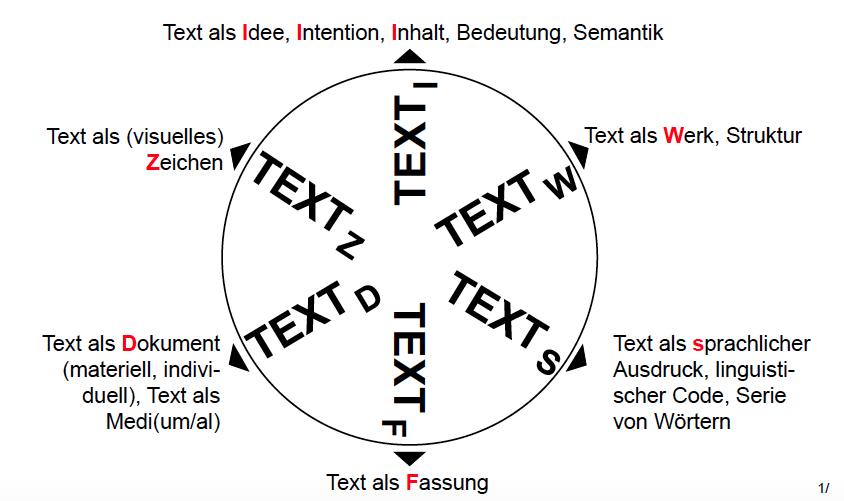
\includegraphics[width=1\textwidth]{img/textrad.png}  
    \caption[Pluralistische Textbegriff als Rad, SAHLE: Digitale Editionsformen: Textbegriffe und Recodierung, S.45-49]{Pluralistische Textbegriff nach SAHLE} \label{fig:textrad}
\end{figure}
\textcolor{red}{Abbildung \ref{fig:textrad} zeigt fünf unterschiedliche Ebenen, die für das Verständnis von Text relevant sind:}
\begin{itemize}
    \item Text als Inhalt: die Idee für den Roman ''Schachnovelle" von Stefan Zweig.
    \item Text als Werk: die Struktur eines Werkes als Sequenz in einem Buch.
    \item Text als Sprache: der ''linguistische Code'' der Schachnovelle als sprachliche Äußerung.
    \item Text als Fassung: verschieden Fassungen des Textes, wie man sie in Zweigs Nachlass findet, wie etwas handschriftlich in einem Maniskript, als Typoskript oder die Korrekturen des Typoskripts. 
    \item Text als Dokument: die materielle Erscheinungsform eines Exemplars in einer Bibliothek.
    \item Text als Zeichen: die Deutung des Visuellen.\footcite[][S.46]{sahle2013digitale}
\end{itemize}
\textcolor{red}{
Die \textbf{kritische Texteditionen} hat eine lange Tradition und wird zur Beantwortung unterschiedlicher Fragestellungen in den Geschichtswissenschaften herangezogen. Es handelt sich um eine Methode, die darauf abzielt, die Abweichungen unterschiedlicher Überlieferungen eines Textes zu bearbeiten und versucht das Material für eine weitere inhaltliche Analyse bereitzustellen. Dabei handelt es sich um eine hermeneutische Methode. In ihr wird die Quelle eingeordnet, dokumentiert und hinsichtlich ihre Authentizität, sowie Vertrauenswürdigkeit überprüft. Gerade das Schaffen von Vertrauen, sodass nicht jede Quelle erneut auf Punkt und Beistrich geprüft werden muss, ist eine Kernaufgabe der Edition und wichtiger Bestandteil des wissenschaftlichen Forschungsprozesses und zur wissenschaftlichen Auseinandersetzung.\footcite[][S.101-144]{aumann1999digital}
\\
\\
Die Idee einer computergestützten Edition wird seit den 1970er Jahren diskutiert. Der Text wird formal in einer Datenbank abgelegt und aufbereitet, damit Abfragen an den Text, oder besser gesagt die Daten, die der Text umfasst, möglich sind. Besonders die Verwendung der Auszeichnungssprache XML und des de facto Standards zur Textauszeichnung TEI (Text Encoding Initiative) hat sich für den Datenaustausch und die Langzeitarchivierung von digitalen Editionen als brauchbar erwiesen. Diese Kombination ermöglicht es editorische Phänomene in Texten mittels einem maschinenlesbaren und kollektiven, also von einer Community weiterentwickelten, Vokabular auszuzeichnen. Nicht eine reine technische Lösung erlaubt es Text formal zu beschreiben und auszuwerten, sondern liegen viele Überlegungen in den Daten selbst und sind so offen für unterschiedliche technische Lösungen.\footcite[][S.180-181]{vogeler2018religion}
\\
Die digitale Edition ist durch folgende Paradigmen\footcite[][S.240-241]{sahle2017dhedition}\footcite[][S.102-108]{ScholgerMartina2018AadS} gekennzeichnet:
\begin{itemize}
\item \textbf{Offenheit:} die digitale Edition erlaubt es den ursprünglichen Text und seiner Annotationen in beliebige weitere Kontexte abzubilden. 
\item \textbf{Vom Produkt zum Prozess:} eine Printfassung ist ein Produkt eines wissenschaftlichen Prozesses. Die digitale Edition aber ist eine Form eines wissenschaftlichen Prozesses, der leicht veränderlich und dokumentierbar ist. Jedochs stellt diese Möglichkeiten noch ein offenes Forschungsthema der digitalen Geisteswissenschaften dar.
\item \textbf{Vernetzung und Zugänglichkeit:} Wissenschaft lebt von der Auseinandersetzung mit anderen und somit ist die Vernetzung von Information und Wissen ein wichtiger Bestandteil. Die digitale Edition, über das Web verteilt und als Prozess verstanden, erlaubt es Inhalte mit andern leichter zu vernetzen.  
\item 
\textbf{Multimedialität:} da es keine Begrenzung gibt, wie in einer gedruckten Edition, können sämtliche Ebenen der Edition in unterschiedlichen Formen zugänglich gemacht werden. Etwa alle Facsimile eine Quelle und nicht nur ausgewählte Seiten, sowie zusätzliche Präsentations und Repräsentationsformen, wie etwas Informationsvisualisierung als Zusammenfassung bestimmter Strukturen in einem Text. 
\end{itemize}
Die Umsetzung einer digitalen Edition ist auch mit neuen Herausforderungen verbunden. Es ist notwendig, dass die langfristige Sicherung der Forschungsdaten, die Zitierbarkeit und Authentizität der Edition gewährleistet sind. Umso mehr ist es notwendig, dass sorgsam methodisches Vorgehen dokumentiert wird und in einer Form als \textit{knowledge domain} abgebildet wird, um eine formale Quellenkritik und -analyse transparent halten zu können.\footcite[][S.306-315]{kropavc2004theorien}
}

\subsubsection{Digitale Edition und Web of Data}

"\textit{Für die geschichtswissenschaftliche Forschung stehen die Inhalte der Dokumente im Vordergrund}."
\footcite[][S.236]{sahle2017dhedition}
\\
\\
\textcolor{red}{
Dieser Aussage von SAHLE folgend bedarf es eines Werkzeuges im Kontext der digitalen Edition, um die Inhalte, die semantischen Strukturen, einer Quelle formal zu beschreiben. Dieses Werkzeug kann, so VOGELER, das \textit{Web of Data} sein und überführt die digitale Edition in eine sogenannte \textbf{''Assertive Edition''}.
\\  
Historiker*innen haben ein besonderes Interesse an ''historischen Fakten''. So Sind Methoden notwendig, deren Ziel es ist, formale Darstellungen der durch den Text vermittelten Informationen in strukturierten Datenbanken abzubilden. Um auch den Ansprüchen der textuellen Ebenen einer Quelle gerecht werden zu können, schlägt VOGELER die Verwendung von eingebetteten Referenzen im TEI-Markup vor, die aus erlauben aus dem Text extrahierte Aussagen in eine RDF-Repräsentation zu überführen. Die Logik diese Referenzen, sprich der jeweilgien Domäne bzw. Forschungsfrage, wird als Ontologie abgebildet.\footcite[][]{vogeler2019assertive}
\\
\\
MEYER vergleicht 52 digitale Editionsprojekte hinsichtlich ihres Expressivitätsgrades und ihres Abstraktionsgrades. Unter Expressivität versteht er wie komplex und ausdrucksstark die Inhalte bzw. Daten in einer Edition ausgedrückt werden und kategorisiert diese in drei Gruppen:  Referenzierung über Normdaten (wie etwa GND oder GeoNames), Aufbereitung als und Verknüpfung mit LOD-Ressourcen und Modellierung interner Bezüge. Die drei Abstraktionsgrade, die den Expressivitätsgraden gegenüberstehen, beschreiben 
\begin{itemize}
\item konkrete Entitäten in stark/schwach strukturierten Texten (Person in einem Roman)
\item konkrete und abstrakte Entitäten in stark strukturierten Texten (Person oder Transaktion in einem Rechnungsbuch) 
\item 
abstrakte Entitäten in schwach strukturierten Texten (philosophisches Konzept in einem Manuskript).
\end{itemize}
Er kommt zu dem Schluss, das \textit{Web of Data} Zugänge, es ermöglichen, tiefergehende Inhalte zu beschreiben und nutzbar zu machen, sieht aber auch noch keine Standardlösung zur Umsetzung des Technologie Stack des \textit{Web of Data} und die damit verbunden Paradigmen in digitalen Editionen.\footcite[][]{meyer2019datenmodellierung}  
\\
\\
Die Anbindung an \textbf{\textit{Linked Open Data}} Hubs, wie beispielsweise \textit{wikidata.org} oder \textit{wiki.dbpedia.org} spielen eine hervorgehobene Rolle in der Vernetzung von Entitäten und Information über Editionsprojekte hinweg.\footcite{wettlaufer2018semanticwebEdition} Dort kann ein stabile und über URIs adressierbare kollaborative Wissensbasis genutzt werden, um Daten auf übergreifende Konzepte zu referenzieren, was für eine weitere Anreicherung, Normalisierung und Aufbereitung für das Finden genutzt werden kann. 
\\
In den folgenden Kapiteln \ref{BK} und \ref{TEI_DEPCHA} wird dieser Zugang am Beispiel des DEPCHA Projektes detaillierter ausgeführt.
}

\newpage
%%%%%%%%%%%%%%%%%%%%%%%%%%%%%%%%%%%%%%%%%%%%%
%%%%%%%%%%%%%%%%%%%%%%%%%%%%%%%%%%%%%%%%%%%%%
\subsection{Die Bookkeeping-Ontology}
\label{BK}

Die \textit{Bookkeeping Ontology}\footnote{\url{gams.uni-graz.at/o:depcha.bookkeeping}, 24.08.2020} ist ein konzeptionelles Modell zur formalen Beschreibung von Transaktionen in historischen Rechnungsunterlagen. Es wurde in einem Ontologie-Engineering-Prozess entwickelt, an dem Historiker*innen, Softwareentwickler*innen und digitale Geisteswissenschaftler*innen beteiligt waren. Die Ontologie befindet sich nach wie vor in der Entwicklung (Stand 2020).



\subsubsection{Grundlagen}
\textcolor{red}{
Ausgangspunkt ist das \textit{Resources, events, agents} (REA) Modell\footcite{mccarthy1982rea}, eine Ontologie, das Buchhaltungsprozessen virtualisiert. Wie der Name sagt, besteht es aus Ressourcen (Gütern, Dienstleistungen, Geld), die in Ereignissen, also Vereinbarungen oder Geschäftstransaktionen, von einem Akteur (Person, Organisation) zum anderen transferiert werden. Im Mittelpunkt jedes REA-Modells steht in der Regel ein Ereignispaar, das durch eine Austauschbeziehung verbunden ist. Eines dieser Ereignisse repräsentiert gewöhnlich den Abgang, die andere eine Empfangen einer Ressource. Im Verkaufsprozess wäre zum Beispiel ein Ereignis ein ''Verkauf'' - bei dem Waren abgegeben werden - und das andere Ereignis ein ''Geldeingang'', bei dem Bargeld empfangen wird. Diese beiden Ereignisse sind miteinander verbunden: ein Geldeingang erfolgt im Austausch gegen einen Verkauf und umgekehrt.
\\
\\
Eine weitere Grundlage bilden die Arbeiten im Kontext von \textit{Modeling Semantically Enhanced Digital Edition of Accounts} (MEDEA), die gerade die Möglichkeiten der Normalisierung und fachwissenschaftliche Annotation, hervorheben. Weiters diskutiere diese Gruppe auch die Rolle der \textit{extensible Business Reporting Language} (XBRL)\footnote{XBRL, \url{https://www.xbrl.org/}, 25.08.2020}, ein XML-basierter Standard ''\textit{for reporting financial information}''. Weiters wird die Ableitung eines konzeptuellen Modells zur Beschreibung von Transaktionen von der Top-Level-Ontology CIDOC-CRM\footnote{CIDOC Conceptual Reference Model (CRM, \url{http://www.cidoc-crm.org/}, 25.08.2020} hervorgehoben.\footcite[][S.9-12]{tomasekmedea} Diese Überlegungen fließen in die Entwicklung der Bookkeeping-Ontology ein. Eine andere Ontologie, die sich in diesem Umfeld bewegt und wirtschaftliche Aktivitäten beschreibt sind die Überlegungen von VAJDA et.al.\footcite[][]{vajda2019toward}
}

\subsubsection{Beschreibung}

In der derzeitigen Fassung definiert die \textit{Bookkeeping Ontology} folgendes:
\\
Eine Transaktion besteht aus mindestens einem Transfer. Jeder Transfer umfasst den Austausch von Dingen, die quantifizierbar sind, von einem Akteur zum anderen. Solche, sogenannte \textit{Measurable}, lassen sich in Geldbeträge, sowie wirtschaftliche Güter unterteilen. Geldbeträge sind dadurch gekennzeichnet, dass sie aus einer Zahl und einer Währung bestehen, wie etwa 10 US Dollar. Weiters gibt es spezielle Formen von Geldbeträgen, wie etwa Steuern, die eine einseitige Geldabgabe definieren, sowie Preise, die den monetären Wert eines Wirtschaftsgutes beschreiben. Die wirtschaftlichen Güter wiederum werden aufgeteilt in Waren -- bestehend aus Menge, Einheit und Art, wie 1 Sack Erdäpfel -- und Dienstleistungen, die eine zeitliche Komponente mit sich bringen können. Die Akteure diesen Transfers können Individuen, Gruppen, Organisationen, Konten oder Kategorien innerhalb von Konten, wie beispielsweise alle Einnahmen einer Stadt auf den Ausschank von Wein, sein. Die Ontologie erlaubt es explizit zu formulieren von wem an wen \textit{Measurables} transferiert werden.
\\
Weiters ist die Verbindung zur historischen Quelle bzw. zum jeweiligen Eintrag wichtiger Bestandteil der Ontologie. Ein Eintrag ist ein Informationsfragment und Beleg eines Ereignisses einer Transaktion in der Vergangenheit. Neben dieser Referenz besteht die Möglichkeit jede Transaktion in seiner zeitlichen, räumlichen und inhaltlichen Dimension, also der Zordnung zu einem bestimmten, durch die Forschungsfrage geprägten, Kontext, zu beschreiben.
\\
Ein Transfer, als Teilbestand einer Transaktion, kann auch von einem Agent, also einer weiteren Person, durchgeführt werden: jemand übernimmt den Transferprozess für jemand anders. Bei der Verbuchung der Transaktion wird eine Transaktion im Sinne der doppelten Buchhaltung auf die Haben oder Soll Seite gebucht. 


\subsubsection{Beispiel}
\label{Beispiel}

\textcolor{red}{
Zu Beginn dieser Arbeit wurde ein Beispiel angeführt, indem ein Akteur, James Haley, am 01.08.1808 ein 1/4 Pfund Pulver, 1 Pfund Munition und 1 Pfund Zucker zum Preis von 2 Schilling und 6 Pence im Laden der \textit{Stagville Plantage} in \textit{North Carolina} käuflich erworben hat. Am folgendem Beispiel wird gezeigt, wie die Annotation des XML/TEI aussieht, um eine Transaktion im Sinne der Bookkeeping-Ontologie zu beschreiben und wie die daraus extrahierten RDF-Triple aussehen.}
\\
\\
\textbf{XML/TEI Beispiel mit Bookkeeping-Annotation}
\\
\\
\textcolor{red}{
Ausgangspunkt ist die Definition eines Containers, der die textuelle Struktur \textit{bk:Entry} und die semantische Struktur \textit{bk:Transaction} zusammenführt. Für die Annotation im XML/TEI wird das Attribut \textit{@ana} verwendet, das eine oder mehrere Interpretationen eines Elements und dessen Inhalts erlaubt. Der \textit{bk:Entry} stellt oft in Rechnungsunterlagen entweder eine Zeile in einer Tabelle oder einen Eintrag in einer Liste dar, ist aber nicht darauf reduziert.
\\
Die hier dargestellte \textit{bk:Transaction} besteht aus zwei \textit{bk:Transfers}: der \textit{bk:Transfers} von Pulver, Zucker und Schrot, und der Fluss des Geldes, also der \textit{bk:Transfers} von 7 Schilling und 6 Pence.
}
\newpage
\begin{lstlisting}[language=XML]
<head> 
  <name ana=''bk:to'' ref=''depcha:stagville''>Stagville</name> 
  <date ana=''bk:when'' when=''1808-08-01''> August 1st 1808</date>
</head> 
<table>
  <head>
   69 <name ana=''bk:from'' ref=''depcha:pers.2''>James Haley</name> 
   <span ana=''bk:status''>Self Dr.</span> 
  </head> 
  <row ana=''bk:entry'' xml:id=''Transaction-0''> 
    <cell> 
     <measure ana=''bk:commodity'' commodity=''wd:Q12861'' quantity=''0.25'' 
       unit=''wd:Q100995''>1/4 lb Powder <measure ana=''bk:price'' 
         quantity=''0.33'' unit=''wd:Q213142''>2/6</measure>
     </measure>
    </cell> 
    <cell> 
     <measure ana=''bk:money'' quantity=''7'' unit=''wd:Q213142''>7</measure>
    </cell>
    <cell> 
     <measure ana=''bk:money'' quantity=''6'' unit=''wd:Q234129''>6</measure>
    </cell>
  </row>
</table>
\end{lstlisting}
\textcolor{red}{
Neben trivialen Markup, wie beispielsweise der Auszeichnung des Datums mittels
\textit{<date ana = ''bk:when''>}, wird der Geldfluss durch die Werte \textit{ana = ''bk:from''} und \textit{ana = ''bk:to''} ausgedrückt. Da in den meisten Quellen dieser Art ein Kauf einer Ware dokumentiert ist, handelt es sich hierbei um die Default-Annahme. Daraus lässt sich schließlich der Fluss von Wirtschaftsgütern -- einer Ware oder Dienstleistung -- ableiten. Einzelne Einträge nennen in der Regel nur einen Akteur einer Transaktion, während die zweite Seite, der Ladenbesitzer des Stagville-Stores, indirekt, aus dem Kontext der Fachwissenschaflter*in, oder auf einer vorangestellten Seite, abgebildet ist. Darüber hinaus kann der Text ''\textit{Self Dr.}'' in der Kopfzeile der Buchung als Transaktions- und Buchungsstatus interpretiert werden und drückt aus, dass die Buchung von dieser Person auf der Sollseite eines doppelten Buchungsstils vorgenommen wurde.
\\
\\
Ein weiterer wichtiger Aspekt ist die Normalisierung von Entitäten wie Personen, Orten, Währungen, Waren oder Dienstleistungen, die im Zusammenhang mit einer solchen Quelle sehr komplex werden können. So sind beispielsweise bestimmte Gewichtseinheiten oder Währungen von regionalen und zeitlichen Unterschieden betroffen. Aufgrund der großen Vielfalt kontextsensitiver Entitäten wird die Normalisierung der Daten durch die Verknüpfung mit \textit{Wikidata.org} oder durch die Erweiterung von Workflows für andere LOD-Vokabulare erreicht. Dies löst natürlich keineswegs die komplexen geschichtswissenschaftlichen Herausforderungen, die mit diesen Normalisierungen einhergehen, die Verwendung von Wikidata könnte aber im Sinne einer großen Wissensbasis ein helfendes Werkzeug sein.
\\
\\
Wikidata erlaubt es eigenständige neue Konzepte zu erstellen, die noch in keinem Vokabular vertreten sind. Das folgende Beispiel verdeutlicht dies: ein weiterer in DEPCHA aufgenommener Datensatz enthält Listen von Waren aus der Stadt Regensburg im 13. Jahrhundert.\footnote{StadtA Regensburg, Kameralien 3} In diesem Datensatz wird der Begriff ''\textit{Scheffen Hafer}'' verwendet und bezieht sich auf eine ganz bestimmte zeitliche und regionale historische Einheit. Der oben beschriebene Arbeitsablauf erlaubt es, solche Begriffe direkt mit \textit{Wikidata.org}-Konzepten zu verbinden, indem die Q-Nummer direkt an ein Attribut angehängt wird. Dieser pragmatische Ansatz wird durch Werkzeuge wie OpenRefine\footnote{Open source Desktop Anwendung zur Datenbereinigung und Datentransformation, \url{https://openrefine.org}, 26.08.2020} für die halbautomatische Identifizierung unterstützt.
\\
Als Ergebnis dieses Workflows extrahiert ein XSL-Transformation die annotierten Strukturen im XML/TEI und +berführt sie in ein RDF, dessen Grundlage die Bookkeeping-Ontologie darstellt. Das folgende RDF/Turtle-Snippet zeigt das verarbeitete XML/TEI:\footcite[][S.10-15]{pollin2019digital}
}
\\
\\
\textbf{RDF-Extraktion}
\\
\\
Danach folgen die RDF-Triple, die aus dieser Annotation extrahiert werden können.
\begin{lstlisting}[]
@prefix bk: <https://gams.uni-graz.at/o:depcha.ontology> .

<#Transaction-0>
  a bk:Transaction> ;
  bk:consistsOf <#Transfer-1>, <#Transfer-2> ;
  bk:when "1808-08-01" ;
  bk:text "1/4 lb Powder 2/6 1 lb Shot 2/6 7 6" .

<#Transfer-1>
  a bk:Transfer ;
  bk:transfers <#Measurable-1> ;
  bk:from <#stagville> ;
  bk:to <#pers.2> .

<#Transfer-2>
  a bk:Transfer ;
  bk:transfers <#Measurable-2-1> ;
  bk:from <#pers.2> ;
  bk:to <#stagville> .

<#Measurable-1>
  a bk:Commodity ;
  bk:unit <wiki:Q100995> ;
  bk:quantity "0.25" ;
  bk:commodity <wikivQ2908004> ;
  bk:price <#Price-1> ;
  bk:text "1/4 lb Powder" .

<#Measurable-2-1>
  a bk:Money ;
  bk:unit <wiki:Q213142> ;
  bk:quantity "7" .
  
 <#pers.2>
  a bk:Between;
  bk:name "James Haley".
  
\end{lstlisting}
\textcolor{red}{
Folgende Abbildung stellt die angeführte Transaktion schematisch dar. Die hellen Knoten definieren Instanzen von Klassen der Bookkeeping-Ontologie, die im Sinen von \textit{Object Properties} mit anderen Instanzen verknüpft sind, bzw. durch weitere Attribute, eben \textit{Data Properties}, beschrieben werden. Angedeutet wird die Normalisierung der Währungen und Maßeinheiten über Wikidata mit den angeführten Q-Identifikatoren. Die RDF-Daten bilden genau diese Graphenstruktur ab, und können so in einer Graphdatenbank verwendet werden.  
}
\begin{figure}[H]
\centering
	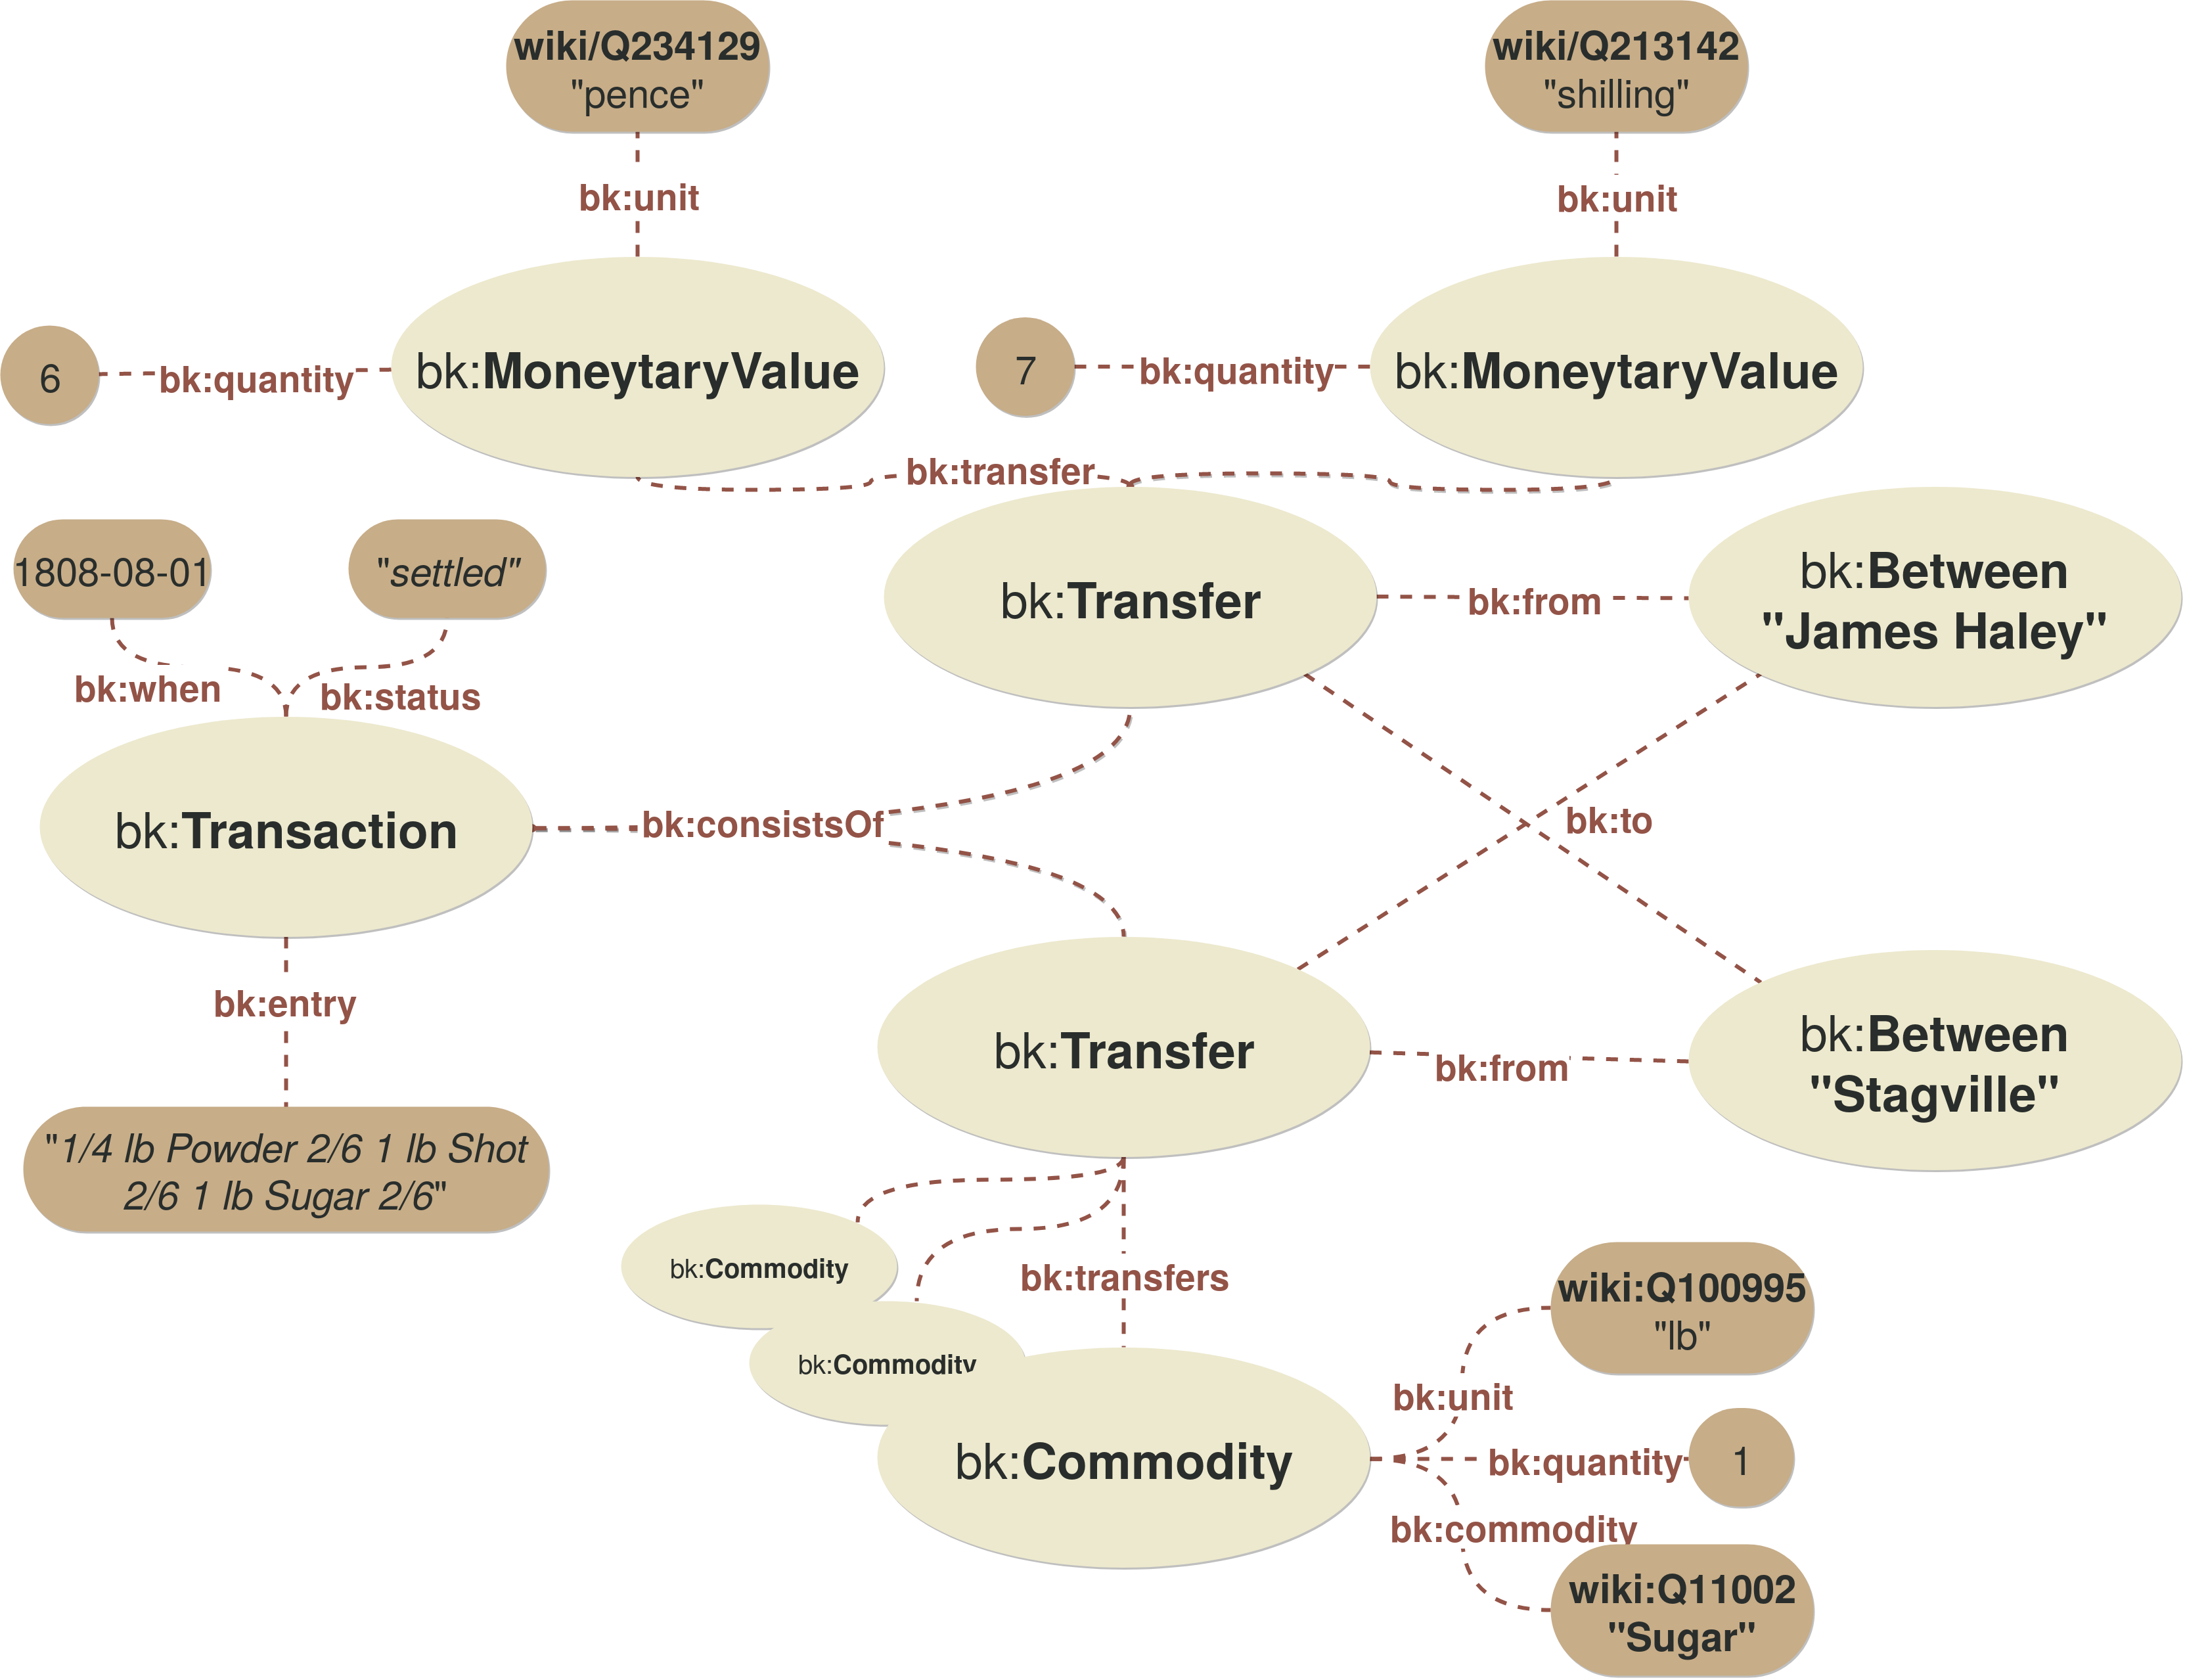
\includegraphics[width=1\textwidth]{img/example.png}  
    \caption[Graphische Darstellung des RDF, eigene Darstellung, 01.06.2019.]{Graphische Darstellung des RDF} \label{fig:example}
\end{figure}


\newpage
\subsection{Informationsvisualisierung}

''\textit{The time of diagrammatic thinking is upon us. We need graphical interfaces for multidimensional and multimedia authoring that take advantage of computers’ abilities to aggregate, synthesize, and organize arguments along multiple axes}''\footcite[][S.119]{burdick2012digital_humanities}
\\
\\
Arbeitet man mit historischen Rechnungsbüchern, so arbeitet man mit einer Vielzahl von Informationsfragmenten. Für Forschungsfragen ist oft der Blick auf das Ganze interessant und so auch die Aggregation und Synthese der einzelnen Belege. BURDICK sieht gerade im Aufkommen der digitalen Geisteswissenschaften die Zeit reif, die Ergebnisse der computergestützten Verarbeitung multidimensional zu visualisieren. Die Informationsvisualisierung ist eine Methode, die dabei helfen kann Erklärungen historischer Ereignisse, die aus der Zusammenschau vieler Quellen und Entitäten zusammenkommen, zu argumentieren und sichtbar zu machen.\footcite[][S.3-5]{frank2018visualisierungswerkzeuge} Sie dient nicht dazu eine ''historische Wahrheit'' abzubilden, die auf einer Zahlenbasis errechnet wurde, sondern kann vielmehr ein Werkzeug im hermeneutischen Prozess sein, um eine Domäne besser verstehen zu können.
\\
\\
Als Visualisierung versteht man -- neben dem eigenständigen Fach aus dem Bereich \textit{Human-Computer Interaction} -- die Anwendung computerbasierter, interaktiver und visueller Repräsentation von abstrakten, nicht-physikalischen Daten, die eine Hilfestellung für den Erkenntnisgewinn sein können. Die Daten können sowohl quantitativer, wie etwa geographische Koordinaten oder Messwerte, sowie qualitativer Natur sein. Die Fachliteratur unterscheidet zwei Herangehensweisen. Wo die \textbf{Scientific Visualization} die Welt so darstellt, wie sie ist, beispielsweise die naturgetreue Darstellung des menschlichen Körpers, wird in der \textbf{Information Visualization} ein Datenbestand in neuen (abstrakten) Informationsräumen, wie etwa in einem Koordinatensystem dargestellt. MUNZER fasst dies zusammen als "\textit{Its scientific visualization when the spatial representation is given. Its Information Visualization when the spatial represenation is chosen}''\footcite[][S.134-153)]{munzner2008process}. Im Falle von Rechnungsbüchern und den Geschichtwissenschaften generell, kann man stets von einer Informationsvisualisierung ausgehen. Eine naturgetreue Darstellung historischer Ereignisse ist nie möglich.

\subsubsection{Voraussetzungen}

Die Menschliche Wahrnehmung ist multimodal. Es entstehen unterschiedliche Repräsentation in unserem Bewusstsein auf Basis der aufgenommen Wahrnehmungen unserer Umgebung. Bei der Umsetzung von Anwendungen der Informationsvisualisierung sind für PREIM und DACHSELT folgende Dimensionen zu berücksichtigen:\footcite[][S.437-440]{preim2010interaktive}
\begin{itemize}
    \item Zielgruppe: für wen ist die Visualisierung konzipiert?
    \item Aufgabe: welches Ziel wird mit der Darstellung verfolgt; was soll dargestellt werden?
    \item Daten: auf welchen Grundlage fußt die Darstellung?
    \item Repräsentation: welche Formen der Repräsentation werden für die Darstellung genutzt?
    \item Medium: wo wird es ausgegeben; wo kann man damit arbeiten?
\end{itemize}
Auf das DEPCHA Projekt gemünzt, wird mit einer Visualisierung das Ziel verfolgt, für ein fachwissenschaftliches Publikum eine größere Menge historischer Information von Transaktionen über das Web so aufzubereiten,  dass aus der Aggregation der historischen Information neue Erkenntnisse gewonnen werden können. So kann die visuelle Repräsentation von historischer Information in den Rechnungsbüchern zur Bearbeitung von relevanten Forschungsfragen herangezogen werden. Die Zielsetzung der Visualisierungen liegt darin, die Dimensionen der Rechnungsbücher, das heißt die beteiligten Akteure, die Wirtschaftsgüter, die Geldbeträge jeweils in ihrem historischen Kontext, für Anwender*innen, im Sinne einer quellenbasierten Arbeitsplattform erfahrbar zu machen. Diese Arbeitsplattform soll Fachwissenschaftler*innen erlauben, sowohl den Einzelbeleg aus der Quelle, als auch die Aggregation der Information einer ausgewählten Menge von Belegen zu erkunden und selbstständig organisieren zu können. Diese zwei Zugangsarten kann man als \textbf{\textit{Close Viewing}}, der ''klassische'' Zugang punktuelle Quellen manuell zu analysieren und \textbf{\textit{Distant Viewing}}, die eine Form der formalen Methodik mit sich bringen muss, bezeichnen.\footcite[][]{hsozkult2014closereading} 
\\
\\
Allgemein kann man sagen, dass das Ziel der Informationsvisualisierung der Gewinn neuer Erkenntnis ist. Wichtig ist das Entdecken neuer Zusammenhänge, die erst in einem größeren Kontext sichtbar werden (\textbf{\textit{Discovery}}), das Treffen von zuverlässigen Entscheidungen (\textbf{\textit{Descision making}}), die explorative Analyse von Informationsräumen (\textbf{\textit{Exploration}}), sowie das Sichtbarmachen von Erklärungen (\textbf{\textit{Explanation}}). Gerade für eine fehlerhafte, unscharfe oder inhomogene Datenbasis kann die menschliche Exploration von Daten sehr effektiv sein.\footcite[][S.439-444]{preim2010interaktive} Das Organisieren in DEPCHA umfasst die Selektion und das Filtern von Ergebnissen, die durch das \textit{Discovery} der Visualisierungen gegeben sind. Die explorative Analyse, sowie eine Sichtbarmachung von Erklärungen durch Darstellungen kann vorher entworfene Thesen zu einem aus einem Rechnungsbuch abgeleiteten Sachverhalt stützen.
\\
Eine weitere Zielsetzung liegt darin, dass eine Visualisierung dabei helfen kann, die Datenqualität der digitalen Edition zu verbessern. Größere Mengen an ähnlich strukturierter Information bergen ein erhöhtes Risiko, dass sich während der manuellen Annotation Fehler einschleichen. Durch die Visualisierung der Daten ist es leichter Workflows aufzusetzen, in dem die Visualisierung des Quellenkorpus genutzt werden kann, um fehlerhafte Transkriptionen oder falsche Zuordnungen bestimmter Entitäten -- wie etwa die Normalisierung von Personen, Gütern oder Maßeinheiten -- besser entscheiden zu können.
\\
\\
Um die notwendige Dimension, nach denen eine mögliche Visualisierung umgesetzt werden kann, festmachen zu können, muss ein Modell definiert werden. Da im Projekt DEPCHA Rechnungsbüchern aus unterschiedlichen Kontexten zusammengeführt werden, bedarf es eines konzeptuellen Modells, um dieses Mapping herzustellen. Die Kategorien, die im Mapping abgebildet werden sollen, entsprechen auch den Dimensionen, die für eine Visualisierung der Informationsobjekte, ihrer Attribute und Relationen, relevant sind. Geldbeträge und Mengenangaben werden als quantitative Daten verstanden, da sie arithmetische Operationen erlauben, wohingegen Kategorien von Gütern und Währungen qualitative Daten darstellen, die für die Beschreibung, Ordnung und Gruppierung dienlich sind.\footcite[][S.448-450]{preim2010interaktive}

\subsubsection{Multidimensionale Rechnungsbücher – Multiple Views und Interaktion}

GLEBA und PETERSEN heben die Vielfalt der Inhalte in Rechnungsbüchern, sowie die Möglichkeiten der ''\textit{interdisziplinären Erschließung der Quelle Rechnungsbuch}'' hervor.\footcite[][S.7-10]{gleba2015wirtschafts} und auch VOGELER sieht in Rechnungsbüchern multidimensionale Quellen.\footcite[][]{vogeler2016content}
\\
Ein Credo der Informationsvisualisierung ist es, eine Domäne in mehreren Dimensionen darzustellen, vom Großen ins Detail zu gehen (\textit{overview first}), dort zu filtern und in die Daten eintauchen zu können, um anschließend auf die Detailebene vorzudringen. Um die Vielfalt der Ebenen und Dimensionen von historischen Rechnungsbüchern auch nutzen zu können, bedarf es auch einer Vielzahl an Repräsentationen. Deswegen bedarf es multipler Perspektiven auf ein Thema. Dies wird in der Informationsvisualisierung als \textit{Multiple Views} zusammengefasst.\footcite[][S.452-462]{preim2010interaktive}
\\
\\
Ein gelungenes Projekt zur Datenvisualisierung wirtschaftlicher Daten, das \textit{Multiple Views} anbietet, ist der \textit{Atlas of Economic Complexity}\footnote{Atlas of Economic Complexity, \url{atlas.cid.harvard.edu}, 09.12.2019}. Es soll stellvertretend für eine moderne Webanwendung stehen, die ähnliche Informationsobjekte repräsentiert. Eine Anlehnung von Darstellungen historischer Information an den \textit{Atlas of Economic Complexity} scheint sinnvoll. So verfügt diese Anwendung über unterschiedliche Visualisierungsformen für Warenexport und -import von Ländern. Sogenannte \textit{Product Treemaps} werden verwendet, um die Größe und Kategorisierung von Exporten und Importen darzustellen, eine \textit{Geo Map} erlaubt die geographische Kontextualisierung dieser Werte auf einer Karte und ein \textit{Stacked Chart} erlaubt es, die Veränderung über die Zeit hinweg zu erfahren. Weiters verfügt die Webseite über mehrere Nutzer*innenfunktionalitäten zum Filtern und Selektieren der Daten. Folgende Abbildung veranschaulicht die \textit{Product Treemap} der Exporte der Vereinigten Staaten von Amerika aus dem Jahr 2016.
\begin{figure}[H]
\centering
	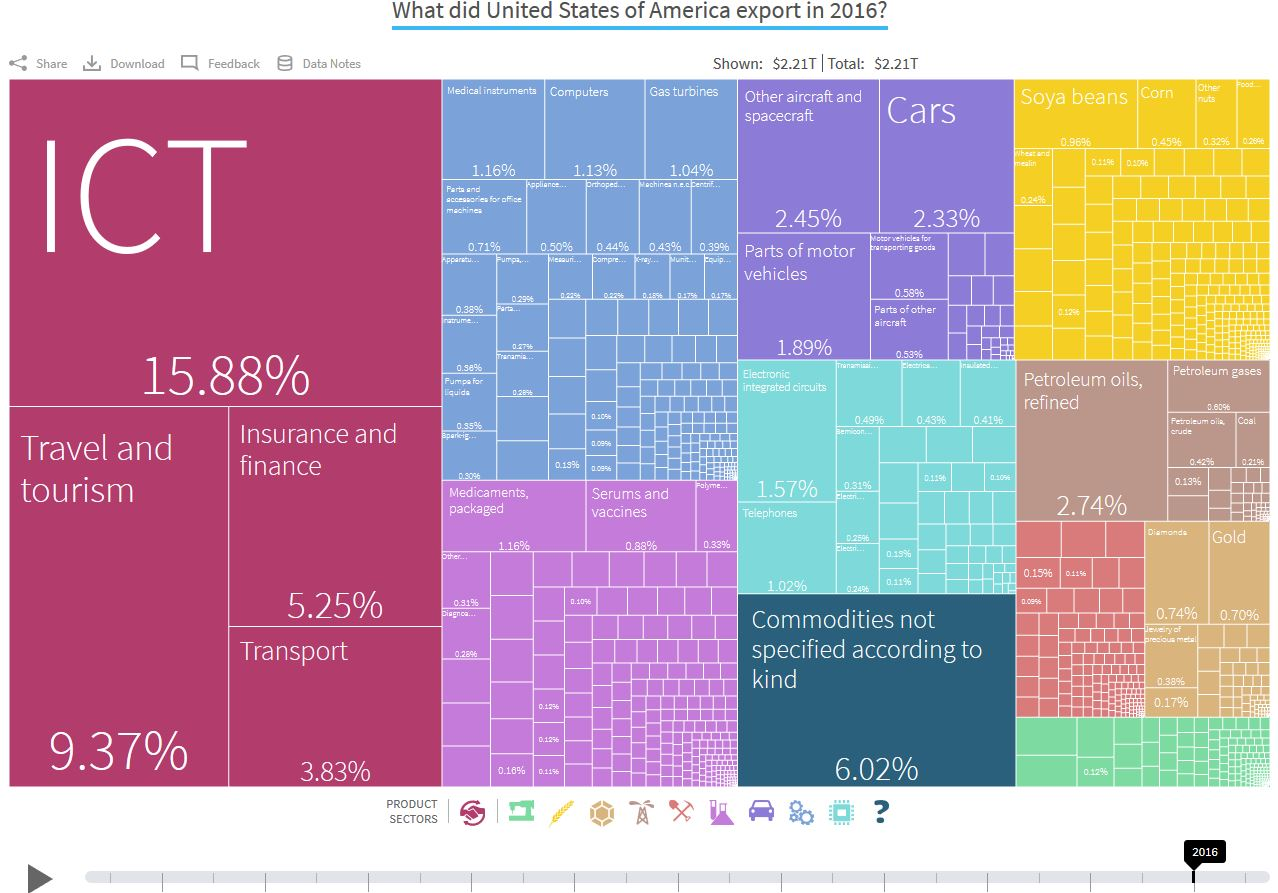
\includegraphics[width=1\textwidth]{img/atlas.jpg}  
    \caption[Screenshot der Product Treemap des Atlas of Economic Complexity, Exporte der USA im Jahr 2016, atlas.cid.harvard.edu 09.12.2019.]{Screenshot der Product Treemap des Atlas of Economic Complexity, Exporte der USA im Jahr 2016} \label{fig:atlas}
\end{figure}
Die \textbf{Treemap}, die man in dieser Abbildung sieht, erlaubt es hierarchische Strukturen und Größenverhältnisse darzustellen. Dazu werden Rechtecke proportional zur Größe der darzustellenden Dateneinheit ineinander verschachtelt. Historiker*innen arbeiten oft mit Klassifikationen, um Information besser ordnen zu können. So erlaubt eine Treemap den schnellen Blick darauf, welche Güter und Dienstleistungen, nach welchen Kategorien geordnet und in welchen Größenverhältnissen zueinander stehen.
\\
Eine weitere Form der Repräsentation sind \textbf{Bar Charts} (Säulendiagramme). Diese Repräsentationsform ist ein klassischer Weg, um Häufigkeitsverteilungen darzustellen, jedoch ist sie auf eine bestimmte Anzahl an Ausprägungen (Säulen) begrenzt. Jede dieser Säulen auf der X-Achse kann beispielsweise ein Geschäftsjahr mit den Einnahmen bzw. Ausgaben in einem Rechnungsbuch darstellen. Da der Zeitraum eines einzelnen Buches sich mit bis zu 15 Säulen abdecken lässt, jede Säule entspricht einem Jahr, kann dies eine geeignete Darstellung sein. Ein \textbf{Stacked Chart} erlaubt es, eine weitere Dimension in ein Bar Chart einzufügen, um Einkünfte und Ausgaben weiter kategorisieren zu können. Beispielsweise könnten diese Dimensionen die einzelnen Akteure sein, die an den Geldflüssen beteiligt sind. Rechnungsbücher können aus einer Vielzahl von Perspektiven betrachtet werden: welche Güter, Akteure und Geldbeträge kommen vor und welche sozialen und gesellschaftlichen Implikationen könnten daraus abgeleitet werden.
\\
\\
Prototypisch wurde auf der in RDF modellierten Datengrundlage mittels SPARQL eine Datenbankabfrage formuliert und das so gewonnene JSON Ergebnis als Input an die Datenvisualisierungssoftware \textit{Tableau Desktop}\footnote{Tableau Desktop, \url{tableau.com/de-de/products/desktop}, 09.12.2019.} übergeben. Bei den folgenden zwei Beispielen handelt es sich um Visualisierungen, wie sie sinnvollerweise für Rechnungsbücher umgesetzt werden könnten.
\begin{figure}[H]
\centering
	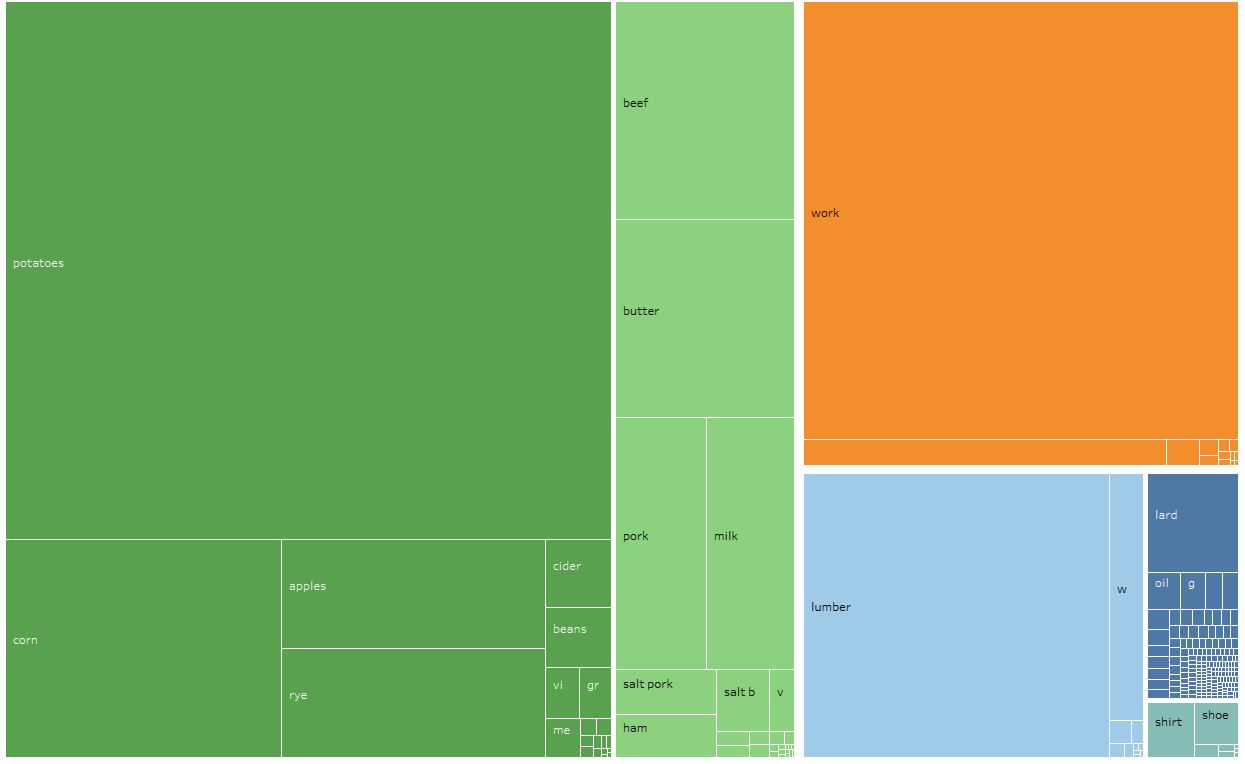
\includegraphics[width=1\textwidth]{img/infovis1.jpg}  
    \caption[Treemap nach Häufigkeit von Waren und Dienstleistungen. Gruppiert nach tierischen (hellgrün) und pflanzliche (dunkelgrün) Lebensmittel, Dienstleistungen (orange), Rohstoffen (hellblau), Textilien (türkis) und sonstigen Waren (dunkelblau), eigene Darstellung, erstellt mit Tableau Desktop]{Treemap nach Häufigkeit von Waren und Dienstleistungen. Gruppiert nach tierischen (hellgrün) und pflanzliche (dunkelgrün) Lebensmittel, Dienstleistungen (orange), Rohstoffen (hellblau), Textilien (türkis) und sonstigen Waren (dunkelblau)} \label{fig:InfoVis1}
\end{figure}
In dieser Ansicht, einer Treemap Ansicht der wirtschaftlichen Güter, entspricht die Größe der Rechtecke der Häufigkeit wie oft ein Gut in allen Transaktionen des \textit{Wheaton Daybooks} vorkommt. Eine besondere Problemstellung dabei ist die Repräsentation bzw. Umrechnung von unterschiedlichen Maßeinheiten auf normalisierte Werte, die dann gegenübergestellt werden können. So stünden 100 \textit{bushel potatoes}, 20 \textit{feet lumber} gegenüber. Deswegen wurde in dieser Darstellung nur die absolute Anzahl, wie oft etwas genannt wird, dargestellt. In dieser Ansicht werden 3 Hauptgruppen unterschieden: Lebensmittel (grün), Dienstleistungen (orange) und Waren (blau). Diese wurden, um eine weitere Hierarchieebene einzufügen, weiter unterteilt in pflanzliche (dunkelgrün) und tierische (hellgrün) Lebensmittel, Rohstoffe (hellblau), Textilien (dunkelblau) und andere Waren (türkis). Im DEPCHA Projekt sind die Hierarchien, nach denen die Rechtecke angeordnet werden, durch Thesauri, die von den Fachwissenschaftler*innen definiert werden, vorgegeben. Diese Hierarchien müssen demzufolge sinnvoll auf die Quellen und die Forschungsfragen abgestimmt werden.
\\
In Abbildung \ref{fig:InfoVis1} zeigt sich sofort der Schwerpunkt der Geschäfte von Wheaton: pflanzliche Produkte, vor allem Kartoffel, Mais, Äpfel und Roggen, sowie Fleisch und Milchprodukte, Arbeit als Dienstleistung und verarbeitetes Holz (\textit{lumber}) als Rohstoff. Daneben gibt es eine Vielzahl von Gütern, die selten gehandelt werden, wie etwa Bücher. Diese befinden sich im stark geschachtelten dunkelblauen Bereich.
\\
\\
Neben den Warenflüssen, sind die Geldflüsse ein zentraler Bestandteil der Daten. Folgende Darstellung zeigt die Geldflüsse an L.M. Wheaton für jedes Jahr. Jede Farbe auf den einzelnen Säulen repräsentiert einen Akteur. Personen wie etwa Wheaton Wheeler (hellroter Balken), ein Verwandter von L.M. Wheaton, kommt sehr regelmäßig in den Laden, kauft aber nur Lebensmittel und Alltagsgegenstände zu niedrigeren Geldbeträgen, gleichzeitig verrichtet er auch öfters Arbeit für L.M. Wheaton.
\\
Es lässt sich daraus schließen, und solche Interpretationen sind die Zielsetzung dieser Darstellungen, dass Wheaton Wheeler aus einem niederen sozialen Status stammt und in einer gewissen Abhängigkeit zu L.M. Wheaton steht. Weiters erhält ein User so einen Überblick, in welchen Jahren niedrigere oder größere Einnahmen zustande kamen, und über die einzelnen Akteure und ihrer Frequenz.
\begin{figure}[H]
\centering
	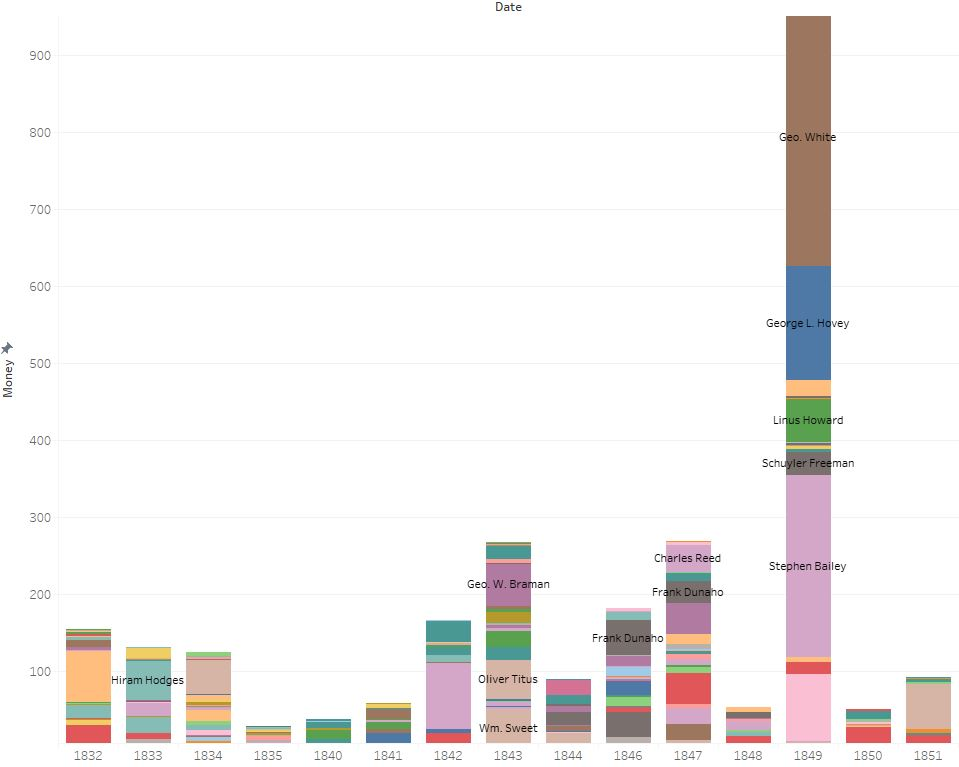
\includegraphics[width=1\textwidth]{img/infovis2.jpg}  
    \caption[Geldfluss nach Jahren (x-Achse) und Summe der Geldflüsse (y-Achse). Stacks nach einzelnen Akteuren, eigene Darstellung, erstellt mit Tableau Desktop]{Geldfluss nach Jahren (x-Achse) und Summe der Geldflüsse (y-Achse). Stacks nach einzelnen Akteuren.} \label{fig:InfoVis2}
\end{figure}

\subsubsection{Informationsvisualisierung und Web of Data}


FRANK\footcite{frank2018visualisierungswerkzeuge} führt 4 Beispiele von Projekten an, die die Methoden der Informationsvisualisierung so nutzen, dass sie zentraler Bestandteil zur Bearbeitung einer geisteswissenschaftlichen Forschungsfrage und zur Überprüfung der Ergebnisse herangezogen werden können. Ein Beispiel daraus ist das Projekt CEWS. Dieses Projekt behandelt multiperspektivische Konfliktforschung mit Fokus auf politikwissenschaftlichen Forschungsfragen. So wird im Projekt Modallogik als formaler Rahmen für die kontrafaktische Analyse von möglichen Konfliktverläufen eingesetzt und die generative Phänomenologie wird zur Analyse der Perspektiven von historischen Akteuren, den Konfliktparteien, auf Konfliktereignisse vorgeschlagen.
\\
\\
Gemeinsam haben alle diese Projekte, dass der Ausgangspunkt für die Visualisierung zum einen Daten sind, zum anderen ein Modell, dass den Daten Struktur verleiht und so die formale Verarbeitung in Hinblick auf eine Forschungsfrage erlaubt. Ein solches Modell kann unter Verwendung von \textit{Web of Data} Technologien und unter Verwendung von \textit{Linked Open Data} beschrieben und formalisiert werden. Beispielsweise werden \textit{Knowledge Graphs} verwendet um explorative Suchen größerer, kontextsensitiver Daten umzusetzen.\footcite{sarrafzadeh2014exploring} 
\\
\\
Es veranschaulicht, welche Ziele und Herausforderungen mit Methoden der Informationsvisualisierung einhergehen. Dabei handelt es sich um ein starke Werkzeug, um bestimmte Inhalte in Sammlungen von historischen Quellen, beispielsweise Rechnungsbüchern, hervorzuheben. Es muss aber auf vielen Ebenen gut durchdacht sein, damit die vergangene ''Wirklichkeit'' nicht verzerrt wird. Von der Forschungsfrage (was soll gezeigt werden), der Darstellung (wie wird es dargestellt), den Daten (woraus wird es erzeugt), sowie der Interaktion damit (was kann ich damit tun) bedarf eines durchdachten Plans. Darstellungen dürfen nicht zu speziell sein und etwas repräsentieren, das nur für eine einzige Forschungsfrage bzw. einzelnes Rechnungsbuch von Interesse ist, dürfen aber auch nicht zu allgemein sein, sodass daraus keine generischen Lösungen ableitbar sind.
\\
\\


%%%%%%%%%%%%%%%%%%%%%%%%%%%%%%%%%%%%%%%%%%%%%%%%%%%%%%%%%%%%%%%%%
\newpage
\section{Zusammenfassung und Ausblick}

\textcolor{red}{
Die Gegebenheiten der Wissensproduktion in der Gesichtsforschung haben sich auf Grund der Digitalisierung gewandelt und beeinflussen wie Geschichte gedacht, erarbeitet und interpretiert wird. Computergestützte Methoden zur Analyse, sowie die Zurverfügungstellung der digitalisierten Quellen, erlauben neue Blicke und neue Möglichkeiten mit den Quellen zuarbeiten. Aber Digitalisierung ist vielmehr ein mächtiges Werkzeug, das die Arbeit mit größeren Datenmengen effizienter gestaltet, nicht aber ein Paradigmenwechsel in den Geschichtswissenschaften.\footcite[][]{koenig2020archive}
\\
In seinem ''Grundriß der Historik'', gibt DROYSEN einen alten, aber immer noch prägenden Überblick über die Geschichtswissenschaft. In der Arbeit mit formalem, digitalen Methoden und Modellen, sowie Informationssystemen für die Geschichtswissenschaft, erscheinen immer noch die Überlegungen DROYSENS sehr relevant. Das historische Denken und Forschen eingeteilt in Heuristik, Kritik, Interpretation und Topik, sprich die Formen der Darlegung der Ergebnisse aus der historischen Forschung, lassen sich auch nach wie vor heute finden. \footcite[][S.85-116]{hardtwig1990studium}
\\
Betrachtet man beispielsweise die Beschreibung der Heuristik bei DROYSEN, so lässt sich vieles davon auf die heutige Arbeit ummünzen. ''Die Kunst der Heuristik ist, das historische Material zu erweitern und zu ergänzen, und zwar:''\footcite[][S.96]{hardtwig1990studium}
}
\begin{enumerate}[label=(\alph*)]
\item ''durch divinatorisches Suchen und Entdecken;'' 
\item ''durch Kombination, [...], durch richtige Einreihung [...]''
\item ''durch Analogie [...]'' 
\item ''durch Hypothese, deren Beweis die Evidenz des Ergebnisses ist [...]''
\end{enumerate}
\textcolor{red}{
ToDo Gegenüberstellen von DROYSENS Heuristik mit Modell - Ontologie - INfomrationsvisualisierung - DEPCHA
\\
\\
Die Bookkeeping-Ontology ist der Versuch der \textit{Kombination}, also der richtigen Einreihungen von Information in Quellen. 
\\
Das Interface von DEPCHA verknüpft mit LOD ist das \textit{divinatorisches Suchen und Entdecken}.
\\
\\
Digital History hat hilfwissenschaftlicehn Charakter. 
\\
Die Arbeit im Projekt DEPCHA zeigt, dass Workflows definiert werden können, damit Information in digitalen Editionen von historischen Rechnungsunterlagen  ausgezeichnet werden kann. Die Bookkeeping-Ontology erlaubt es Transaktionen, also den Fluss von wirtschaftlichen Gütern und Geldbeträgen von einem Akteur zum anderen zu beschreiben. Diese Formalisierung, mittels Ontologie des \textit{Web of Data}, dient als Grundlage für weiter Formen der Analyse. Dazu eigenen sich XML/TEI, um auch die textuelle Strukturen eine Quelle zu beschreiben, wie RDF, das die Transaktion an sich in Form von Triples ermöglicht. Die Entwicklung der Bookkeeping-Ontology ist ein iterativer und ncith abgeschlossener Prozess. Ziel letztendlich ist es, möglichst alle Phänomene, die eng mit wirtschaftlichen Transaktionen verbunden sind, formal in diesem Modell abzubilden.
\\
\\
Folgende Vorteile gehen mit der Verwendung von Ontologien einher:}
\begin{itemize}
\item Ein gemeinsames Vokabular bzw. Modell erleichtert die Kommunikation in der Wissensproduktion und kann vn Fachkolleginnen und Kollegen nach genutzt werden.
\item Die Wiederverwendung eines Modells befördert den fachwissenschaftlichen Diskurs, in dem bestehende Konzepte kritisiert und fehlende Konzepte ergänzt werden können. Dies führt zu einem allgemein akzeptierten und verständlicheren konzeptionellen Modell.
\item Linked Open Data, wie etwa auf einem Hub wie Wikidata, ermöglicht Interoperabilität der Daten in verschiedenen wissenschaftlichen Disziplinen. Die so entstanden Synergien, die die Pflege und Entwicklung von Standards vermeintlich erlaubt die Implementierung von generischen Retrieval-, Analyse- und Visualisierungsfunktionalitäten, die den projektspezifischen Anwendungsfällen angepasst werden können. 
\end{itemize}


\newpage
\bibliographystyle{jurabib}
\bibliography{literatur}
\newpage
\listoffigures

\end{document}
